% Template by Matteo Russo, 11/03/2024

% --------------------------
% ---- DECLARE PACKAGES ----
% --------------------------
\documentclass[a4paper, oneside, openright]{book}
\usepackage[T1]{fontenc} % Font encoding, T1 = it
\usepackage{lmodern}
\usepackage[final]{microtype} % Better line breaking, reduces overfull hboxes
\usepackage{multicol} % Used in title page
\usepackage[utf8]{inputenc} % Input encoding
\usepackage[english]{babel} % English as main language
\usepackage{blindtext}
\usepackage{graphicx}
\usepackage[a4paper,top=2.5cm,bottom=2.5cm,left=3cm,right=3cm]{geometry} % Page layout
\usepackage[fontsize=13pt]{scrextend} % Font size
% \usepackage{graphicx} % duplicate removed
\usepackage[parfill]{parskip} % Disable indent on paragraph skip
% \usepackage[hang,flushmargin]{footmisc} % Disable indent in footnotes
\usepackage{titlesec}
\usepackage{minted} % Used for code
\usepackage{float}
\usepackage[font=scriptsize, skip=5pt, justification=centering]{caption} % Caption/image space
\usepackage[style=authoryear-ibid,backend=biber]{biblatex}
\usepackage[immediate]{silence}
\WarningFilter[temp]{latex}{Command} % silence the warning
\usepackage{sectsty}
\DeactivateWarningFilters[temp] % So nothing unrelated gets silenced
\usepackage{hyperref} % Clickable index
% \usepackage[justification=centering]{caption} % duplicate removed; options merged above
\usepackage{csquotes} % Babel dependency
\usepackage[bottom]{footmisc} % Footnotes positioning

% ------------------------
% ---- DOCUMENT SETUP ----
% ------------------------
\pagestyle{plain}
\raggedbottom % Layout on uncomplete pages
\emergencystretch=2em % Allow extra stretch to avoid overfull lines


\titleformat{\chapter}[display]
    {\normalfont\huge\bfseries}{\chaptertitlename\ \thechapter}{10pt}{\LARGE}
\titlespacing*{\chapter}{0pt}{0pt}{20pt}
\chaptertitlefont{\fontsize{22pt}{30pt}\selectfont}

\hypersetup{ % Link colour
    colorlinks,
    citecolor=black,
    filecolor=black,
    linkcolor=black,
    urlcolor=black
}

% \renewcommand{\footnoterule}{ % Footnote dividing line layout
%   \kern -3pt
%   \hrule width \textwidth height 1pt
%   \kern 2pt
% } 
\renewcommand{\footnotesize}{\fontsize{11pt}{13pt}\selectfont} % Footnote font layout
\setlength{\footnotesep}{0.5cm} % Footnote spacing
\setlength{\skip\footins}{1.5cm} % Footnote/body spacing

\DeclareUnicodeCharacter{02BC}{}

% ------------------------
% ---- DOCUMENT START ----
% ------------------------
\addbibresource{bibliography.bib} % Bibliography import
\begin{document} % Document start
\pagenumbering{gobble} % No page numbering
\begin{titlepage}
%\begin{figure}
%    \hfill
%    
\includegraphics[height=2cm]{Figures/logo_tv.png}
%    \hfill
%    
\includegraphics[height=2cm]{Figures/logo_larm.png}
%\end{figure}

%\begin{minipage}{1\textwidth}
%    \begin{multicols}{2}
%        
\includegraphics[height=2cm]{Figures/logo_tv.png}
%        
%         \columnbreak
%         \columnbreak
%
%         \begin{flushright}
%            
\includegraphics[height=2cm]{Figures/logo_larm.png}
%         \end{flushright}
%    \end{multicols}
%\end{minipage}


\begin{center}
    \vspace{6mm}
    \large{UNIVERSITÀ DEGLI STUDI DI ROMA TOR VERGATA}
    \vspace{3mm}
    \\ \normalsize{MACROAREA DI INGEGNERIA}
    \vspace{12mm}
    \\ 
\includegraphics[height=3cm]{Figures/logo_tv.png}
    \vspace{12mm}
    \\ \normalsize{CORSO DI STUDI IN}
    \vspace{3mm}
    \\ \normalsize{Mechatronics Engineering/Ingegneria per l'Energia e l'Ambiente}
    \vspace{6mm}
    \\ \normalsize{TESI DI LAUREA IN}
    \vspace{3mm}
    \\ \normalsize{Robot Mechanics/Meccanica Applicata alle Macchine}
    \vspace{12mm}
    \\ \normalsize{TITOLO}
    \vspace{6mm}
    \\ \LARGE{\textbf{THESIS TITLE}}
    \\ \LARGE{\textbf{LINE 2}}
\end{center}

\vspace{24mm}

\begin{minipage}[t]{1\textwidth}
    \begin{multicols}{2}
    	{\normalsize{\textbf{Relatore:}}{\normalsize\vspace{1mm}
        \\ \normalsize{Prof. Matteo Russo}}} \\ 

        {\normalsize{\textbf{Correlatore:}}{\normalsize\vspace{1mm}
        \\ \normalsize{Name Surname }}} \\
        
         \columnbreak
         \columnbreak

         \begin{flushright}
            {\normalsize{\textbf{Candidato:}}{\normalsize\vspace{1mm}
            \\ \normalsize{Name Surname}\\
            \normalsize{Matricola  123456}}} \\
         \end{flushright}
    \end{multicols}
\end{minipage}

\vspace*{\fill}

\begin{center}
        \normalsize{Anno Accademico 2023/2024}
\end{center}

\end{titlepage}
 % FRONT PAGE
\cleardoublepage
\thispagestyle{empty}
\vspace*{\stretch{7}}
\begin{flushright}
\itshape Insert dedication (optional)\\ \vspace{5mm}
Part 2.
\end{flushright}
\vspace*{\stretch{2}}
\cleardoublepage % Dedication page
 \chapter*{\textbf{Acknowledgments}}

Insert acknowledgments here (optional) % Acknowledgments page
 \chapter*{\textbf{Abstract}}

Set the story, insert short abstract of the thesis (1 page).

Don’t forget to read the university guidelines and respect all the deadlines (assignment module, graduation date and registration, thesis deadline etc.)!
 % Abstract
\tableofcontents  % Index generation
\newpage % New page
\pagenumbering{arabic} % Page numbering on for main thesis body
\setcounter{chapter}{0} % Introduction counts as chapter 0
% ------------------
% ---- CHAPTERS ----
% ------------------


{\fontsize{20}{26}\selectfont\textbf{Introduction}}


Agriculture has long been the backbone of human civilization, yet it faces mounting pressures that threaten its sustainability and efficiency. One such challenge lies in the harvesting of delicate and high-value crops such as asparagus sprouts, a task that demands precision, adaptability, and real-time decision-making. Traditionally, this process relies on human laborers who painstakingly identify, pick, and place each sprout into collection bins, a labor intensive endeavor constrained by fatigue, rising costs, and a shrinking workforce. This situation underscores a critical problem: the absence of intelligent, scalable systems capable of replicating human dexterity and judgment in the unpredictable, unstructured environment of a field. To address this gap, this thesis proposes an autonomous robotic system driven by advanced technologies: a 3D stereo camera to generate point cloud data, a neural network to classify sprout features,  to interpret complex data and control a robot arm for picking and placing asparagus sprouts. This integration of robotics, computer vision, and artificial intelligence aims to revolutionize agricultural automation.


The necessity of this research is rooted in the urgent challenges facing modern agriculture. As the global population rises to 10 billion by 2050, the demand for food production intensifies, while the availability of arable land and labor decline. Asparagus, valued for its nutritional properties and economic return, exemplifies these difficulties: its sprouts require selective harvesting based on size, maturity, and condition, a task ill-suited to rigid, reprogrammed robotic systems. Labor shortages, driven by urbanization, aging rural populations, and economic pressures, further exacerbate the issue, leaving farmers struggling to maintain productivity. This system offers a solution by reducing the dependence on human labor, enhancing efficiency, and ensuring consistent crop quality. By processing 3D point-cloud data from stereo cameras, classifying sprout attributes with neural networks, and leveraging LLMs for adaptive decision making and robotic control, this approach tackles the complexity of field-based harvesting with unprecedented sophistication.


This work is more relevant today than ever because of the convergence of technological advancements and societal needs. Recent breakthroughs in LLMs, such as their ability to process multi modal data and generate context-aware responses, have opened up new possibilities for real-time decision making in dynamic environments. Coupled with improvements in affordable 3D imaging and robotic hardware, these tools enable a level of autonomy previously unattainable. Meanwhile, climate change and resource scarcity increase the urgency for sustainable farming practices, making intelligent automation a critical tool for resilience. In contrast, achieving this feat was prohibitively difficult in the past. Earlier robotic systems lacked the computational power and sensory integration needed to navigate the variability of natural settings: mud, uneven terrain, and irregular crop growth confounded simplistic algorithms. Computer vision struggled with poor resolution and limited depth perception, while decision-making models were too rigid to adapt to unforeseen conditions. The absence of LLMs meant that that robots could not interpret complex, unstructured data or learn from diverse inputs, rendering them ineffective for tasks requiring human-like judgment.

The benefits of this system extend widely, promising trans-formative impacts for humanity and agriculture. For farmers, it reduces labor costs, mitigates workforce shortages, and boosts productivity, enabling them to meet growing food demands efficiently. By automating repetitive, physically demanding tasks, it improves worker well-being and reallocates human effort to strategic roles like crop planning. Environmentally, it supports sustainability by optimizing harvest timing, reducing waste, and minimizing resource use. On a broader scale, this technology could reshape agricultural practices, offering a blueprint for automating other crops and fostering resilient food systems. By bridging robotics, vision, and LLMs, this thesis not only solves a specific challenge but also pioneers a future where intelligent machines enhance our capacity to feed the world.



\chapter{Robots in agriculture}
\section{Robotics in Agriculture}
In 2025, agricultural robotics is at the forefront of transforming farming practices with cutting-edge technology. Key advancements include fully autonomous tractors, like John Deere's 2025 models, which perform tillage functions without human intervention, increasing efficiency and reducing labor costs [\cite{DeereCES2025}]. Precision harvesting robots, such as those from Harvest CROO, address labor shortages by picking crops like strawberries with precision and speed, reducing post-harvest losses. Drones play a crucial role in crop monitoring and precision spraying, enabling farmers to make data-driven decisions and optimize resource use [\cite{BuiltInAgRobots}]. Sophisticated weeding and planting robots, like Lettuce Bot from Blue River Technology (now part of John Deere), reduce herbicide use and manual labor by autonomously thinning and weeding fields [\cite{Robovision2025}]. 

\subsection{Robotic manipulators in agriculture}
The state-of-the-art in agricultural robotics encompasses a wide range of applications, each addressing specific challenges in farming. Below, we detail the major categories and examples:
Autonomous Tractors and Vehicles:
One of the most significant developments is the introduction of fully autonomous tractors. For instance, John Deere revealed new autonomous machines at CES 2025, with driverless autonomy systems available for model year 2025 and newer 8R and 9R tractors, initially for tillage functions [\cite{DeereCES2025}]. These tractors can operate without human intervention, reducing labor costs and increasing efficiency. This aligns with the trend of precision farming, where GPS and AI enable precise navigation and task execution. In general, application of robotics in agriculture can be divided into two sections:






\textbullet \,\textbf{ Precision Harvesting Robots}:
Harvesting robots are transforming labor-intensive tasks, particularly for delicate crops. Companies like Harvest CROO specialize in strawberry harvesting robots that can navigate uneven terrain and pick at human speed, addressing labor shortages and minimizing waste [\cite{BuiltInAgRobots}]. These robots are designed to handle soft crops, reducing post-harvest losses and improving yield efficiency. Another example is the Lettuce Bot from Blue River Technology (acquired by John Deere in 2017), which autonomously thins and weeds lettuce fields, reducing reliance on herbicides . Aotearoa New Zealand’s apple industry faces labor shortages for skilled tasks like thinning, prompting the development of an automated robot that scans both sides of tree canopies to accurately map fruitlets (81\% accuracy) and estimate size (5.9\% RMSE). The system addresses visibility challenges in dense foliage, proving more effective than single-sided scans (73.7\% accuracy) as shown the \ref{fig:applerobot} .

\begin{figure}
    \centering
    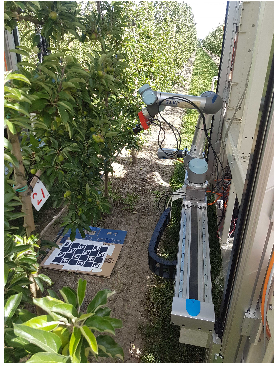
\includegraphics[width=0.5\linewidth]{pictures/robot_pickingapple.png}
    \caption{Internal view of one of the UR5 robotic arms mounted on the linear rail system used to scan the apple trees. [\cite{robotApple}]}
    \label{fig:applerobot}
\end{figure}

This research presents a cooperative grape-harvesting system using two heterogeneous robots—an 'expert' for picking and a 'helper' for transport—to address farm labor shortages and improve efficiency. Field experiments validated the navigation and collaboration strategy, while future enhancements explore logic-based decision-making for autonomous agricultural robots[\cite{robot_grape}].
\begin{figure}
    \centering
    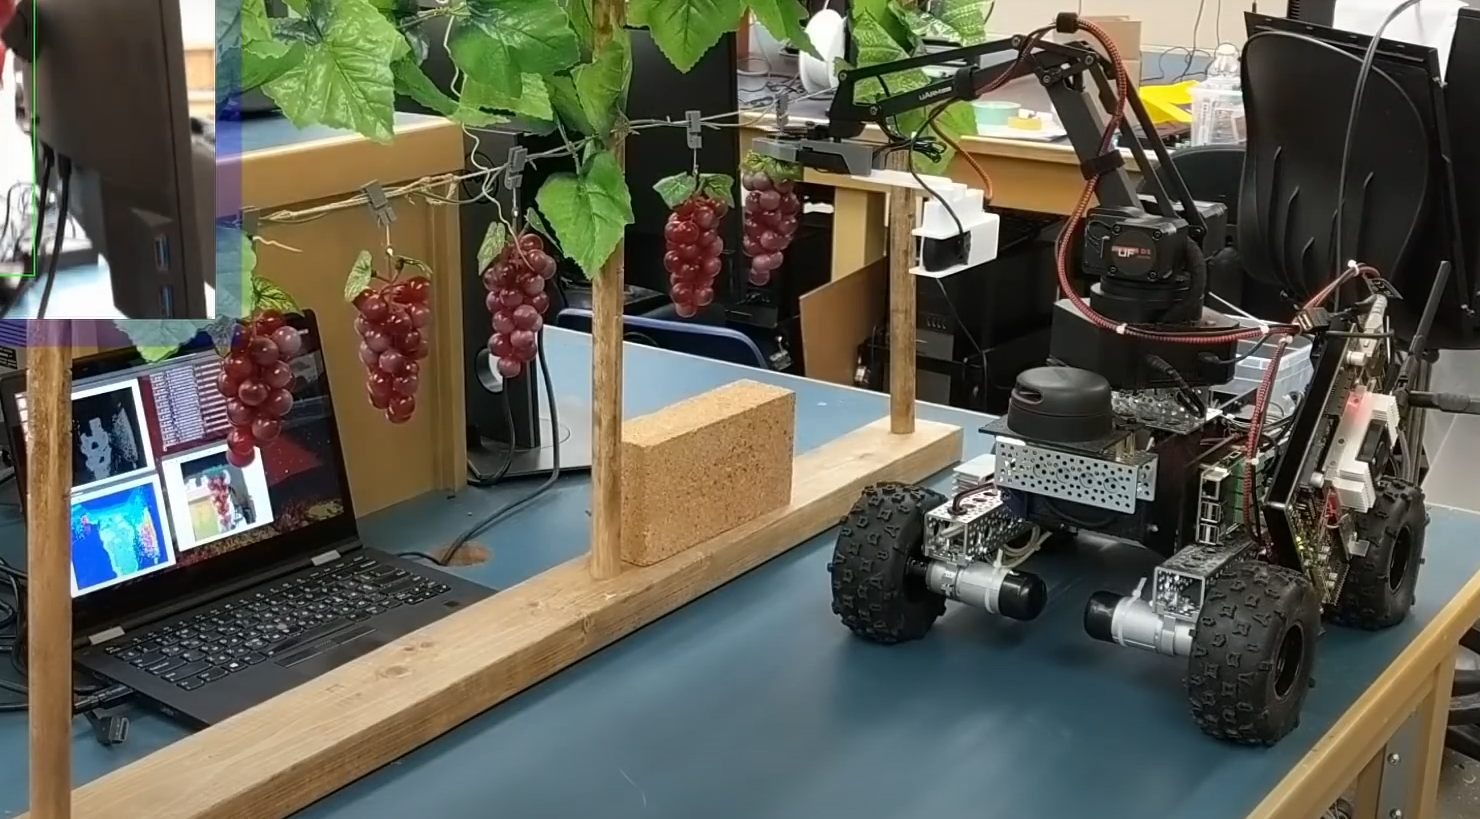
\includegraphics[width=0.75\linewidth]{pictures/grape_robot.png}
    \caption{experimental robot arm picking grapes in lab setup[\cite{robot_grape}]}
    \label{fig:enter-label}
\end{figure}


SWEEPER, the pioneering sweet pepper harvesting robot, achieves 61\% success in optimized greenhouse conditions with 24-second harvest cycles, proving robotics' potential while highlighting the need for crop adaptation. Its commercial-scale testing (262 fruits) reveals critical trade-offs between speed, accuracy, and real-world agricultural constraints[\cite{SweeperProject}].

\begin{figure}
    \centering
    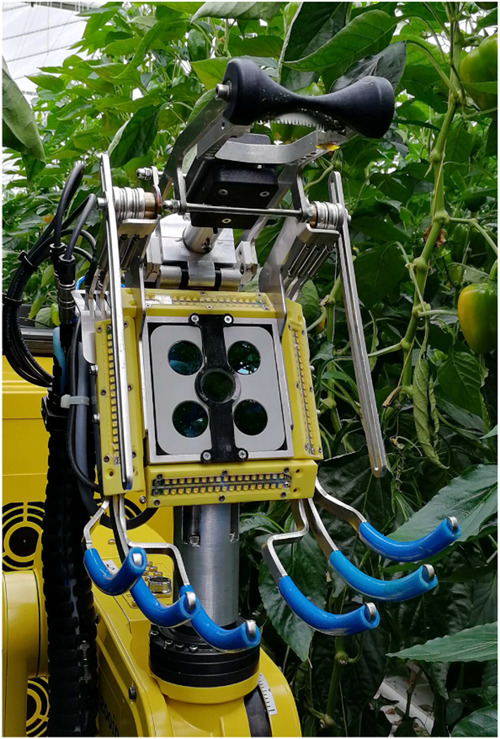
\includegraphics[width=0.5\linewidth]{pictures/bell_pepper.jpg}
    \caption{sweeper robot picking bell pepper}
    \label{fig:enter-label}
\end{figure}

\textbullet \,\textbf{ Weeding and Planting Robots}:
Robotic systems for weeding and planting are becoming more sophisticated, addressing the need for precision and reduced chemical use. The OMEGA robot from Terra Robotics, for example, uses laser technology for autonomous weeding, eliminating the need for chemical herbicides and promoting organic farming [\cite{TerraRobotics}]. Planting robots, often equipped with GPS, ensure optimal seed spacing and depth, improving crop uniformity and yield. These innovations are crucial for sustainable agriculture, reducing environmental impact and labor costs. Carbon Robotics develops AI-powered agricultural robots, specializing in autonomous weed control systems using laser technology to enable sustainable, precision farming. Their flagship product is the 'LaserWeeder' designed to reduce herbicide use while improving crop yields[\cite{CarbonRobotics}].

\subsection{Compliant Grippers in Agricultural Robotics}
The development of effective robotic end-effectors for horticulture remains a significant challenge due to the irregular shapes, fragile textures, and variable sizes of fruits and vegetables. While robotic grippers have been studied for decades, most existing designs are narrowly tailored to single crops like tomatoes or strawberries, limiting their versatility in real-world agricultural applications. Compliant materials emerge as a promising solution, enabling end-effectors to conform gently to produce surfaces, distribute pressure evenly, and minimize damage during handling. Traditional rigid fingers, though mechanically simple, lack adaptability, while articulated designs introduce control complexity without guaranteeing reliability. This study focuses on medium-sized spherical fruits (e.g., apples, tomatoes) with diameters of 40–100 mm, using ripe tomatoes—a worst-case scenario due to their low Young’s Modulus (2.32 MPa)—as a benchmark for gripper design[\cite{russo2017design}]


\begin{figure}
    \centering
    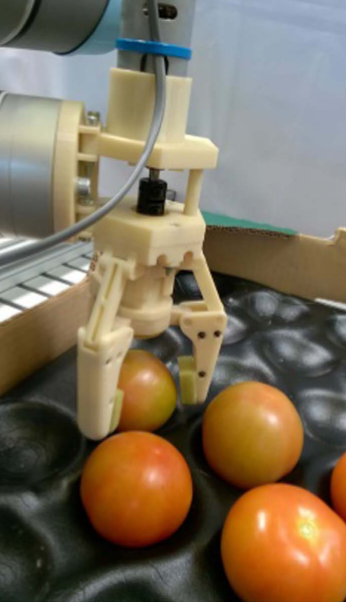
\includegraphics[width=0.5\linewidth]{pictures/tomato_gripper.png}
    \caption{testing a gripper design on different quality of tomatos [\cite{russo2017design}]}
    \label{fig:enter-label}
\end{figure}


this study introduces eight innovative 1-degree-of-freedom end-effectors based on deployable scissor mechanisms, which can compactly fold and expand to harvest single or multiple fruits while offering both direct-fruit and stem-holding separation methods. Validated through 3D-printed prototypes and simulations, these designs demonstrate a 40\% efficiency improvement over conventional approaches, with broader applications extending to tasks like underwater harvesting of sea cucumbers, marking a significant step toward scalable and adaptable robotic farming solutions[\cite{differentDesign}]. The proposed design can grow and twine around target vegetables like bok choy (generating 4-10 N pulling force) while adjusting grip tightness based on contact points, demonstrating versatility across leafy, podded, and gourd vegetables. This smart gripper technology not only advances vertical farm automation but also shows potential for diverse applications in warehousing and food handling industries due to its ability to grasp objects of varying sizes, shapes, and weights[\cite{gripper3}].This paper presents a robotic gripper featuring a three-finger, variable-angle design for harvesting spherical and cylindrical fruits (e.g., cherry, loquat, zucchini). The gripper’s two rotatable fingers, driven by synchronous gears, adapt to diverse fruit sizes (9–122 mm diameter, 8–300 g weight), while kinematic analysis optimizes driving force-to-gripping force conversion for stable, damage-free harvesting. Experimental validation with driving speeds of 5–15 mm/s confirmed reliable performance, with no surface damage observed, addressing key challenges of contact area and force control in agricultural robotics[\cite{multipurpuse_gripper}].

\begin{figure}
    \centering
    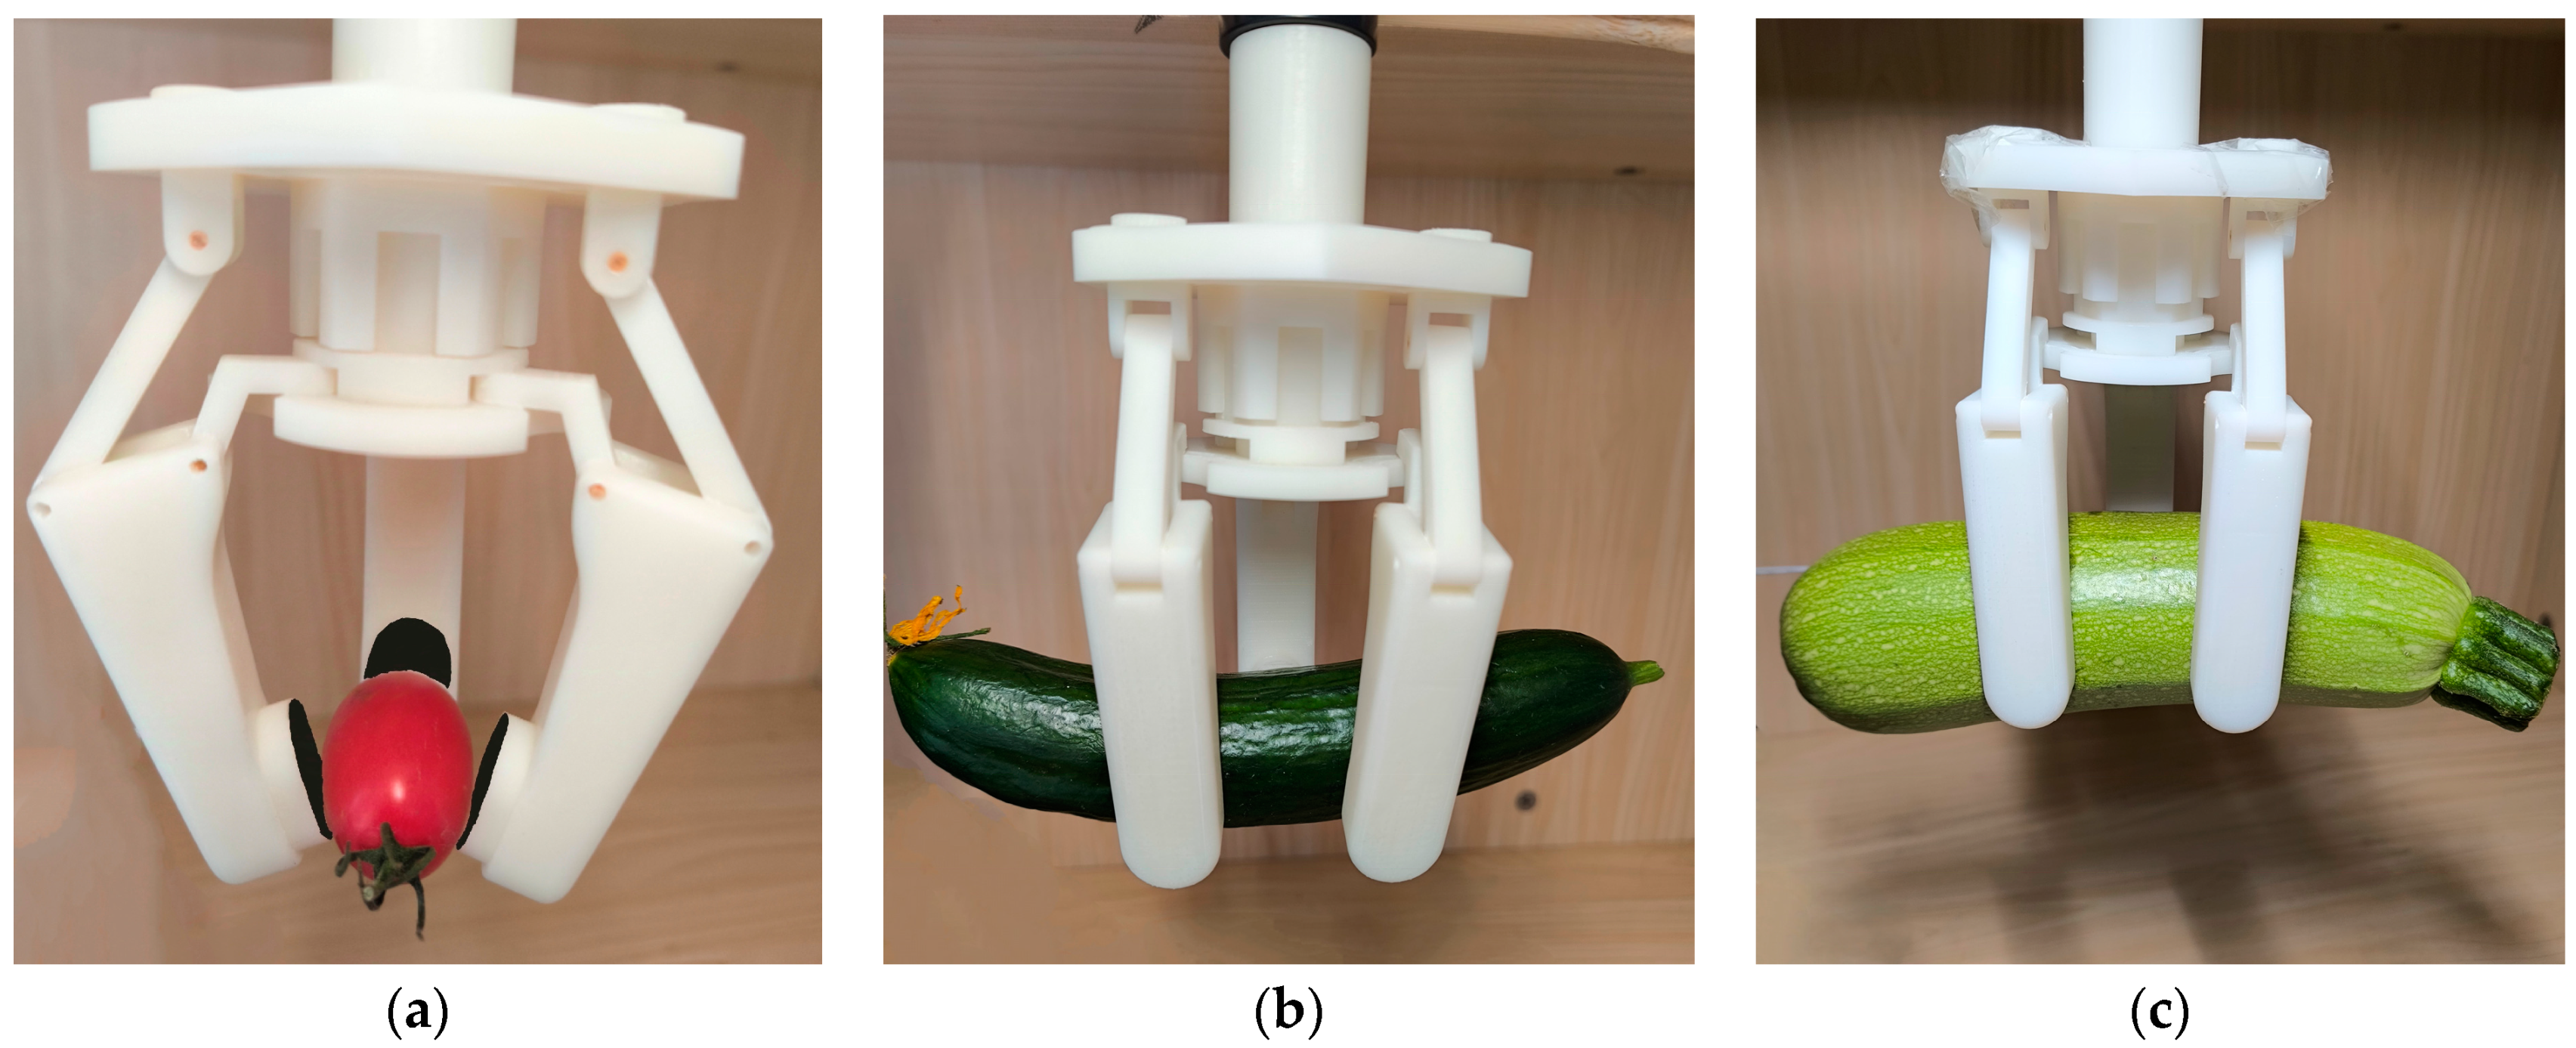
\includegraphics[width=1\linewidth]{pictures/gripper_different_shape.png}
    \caption{Grasping states of different long column strip objects: (a) cherry, (b) loquat, and (c) zucchini.[\cite{multipurpuse_gripper}]}
    \label{fig:enter-label}
\end{figure}

Based on these study, I can conclude that the design for the asparagus gripper should requires a more sophisticated gripper design compared to other fruits/vegetables:

\textbullet \,\textbf{ Unique Morphology}:
Unique Morphology: Asparagus spears have a long, slender, and tapered shape with delicate tips, demanding precise force distribution along their length to avoid bending or snapping, unlike spherical fruits where grip forces can be evenly distributed.\\
\textbullet \,\textbf{ Fragility and Surface Sensitivity:}
Fragility and Surface Sensitivity: The tender skin and high moisture content of asparagus make it prone to bruising or peeling under excessive pressure, necessitating compliant materials and real-time force feedback to adjust grip dynamically.\\
\textbullet \,\textbf{Harvesting Complexity :}
 Asparagus grows at varying angles and densities in the field, requiring grippers with advanced spatial awareness (e.g., 3D vision) and adaptability to selectively harvest mature spears without disturbing adjacent plants.


\section{Comprehensive Analysis: Rationale for \newline Robotics in Asparagus Farming}

Asparagus sprouts, commonly referred to as spears, are harvested primarily by hand in most parts of the world, a method rooted in the crop’s delicate nature and the need for selective picking. Asparagus (Asparagus officinalis) is a perennial plant, with spears emerging from underground crowns in spring and early summer. Harvesting occurs daily or every few days during the 6- to 8-week season, depending on climate and growth rates, as spears must be collected when they reach an optimal height (typically 5-9 inches) before they "fern out" and become fibrous. Workers use knives or snap the spears by hand just above or below the soil surface, depending on market preferences—snapping yields an all-edible product, while cutting below ground adds weight but includes a tougher base often discarded.


In major producing regions like the United States (Michigan, California), Peru, and China, manual labor dominates due to the precision required to assess spear quality and maturity. For instance, in the U.S., where annual production hovers around 20,000-25,000 acres, small-scale farms (often under one acre) rely on seasonal workers or family labor. Larger operations may employ migrant workers, particularly in labor-intensive periods. In contrast, countries like Peru, a leading exporter, benefit from lower labor costs, enabling them to dominate global markets with hand-harvested asparagus. The process involves workers bending or kneeling in fields, collecting spears into buckets or crates, which are then transported for washing, sorting, and packing—often still by hand for premium fresh markets.


Economic and Social Effects
Economically, manual asparagus harvesting has significant implications. It’s labor-intensive, with labor costs constituting a large portion of production expenses—sometimes up to 50 or more, depending on wages and region. In the U.S., where farmgate value ranges from 70-100 million annually, growers face competition from imports (e.g., Peru and Mexico supply 80-90 of U.S. consumption), which depresses domestic prices and squeezes margins. Small-scale farmers benefit from niche markets like farmers' markets or CSAs, fetching premium prices (3-5 per pound), but larger producers struggle with scale and cost efficiency. Rising labor costs, driven by minimum wage increases or labor shortages, further challenge profitability, especially as U.S. acreage has declined to a third of its level two decades ago due to import pressure.
Socially, the reliance on manual labor ties asparagus production to broader workforce dynamics. In developed nations, it sustains seasonal employment, often for migrant or rural communities, providing income but also perpetuating low-wage, physically demanding jobs. In the U.S., for example, many workers are immigrants, highlighting issues of labor rights, housing, and access to services. In developing countries like Peru, asparagus harvesting supports rural livelihoods but can reinforce economic disparities, as smallholders may lack bargaining power against exporters. Gender roles also emerge—women often participate in sorting and packing, while men dominate field work—reflecting traditional divisions with varying social equity implications. Additionally, 

\begin{figure}
    \centering
    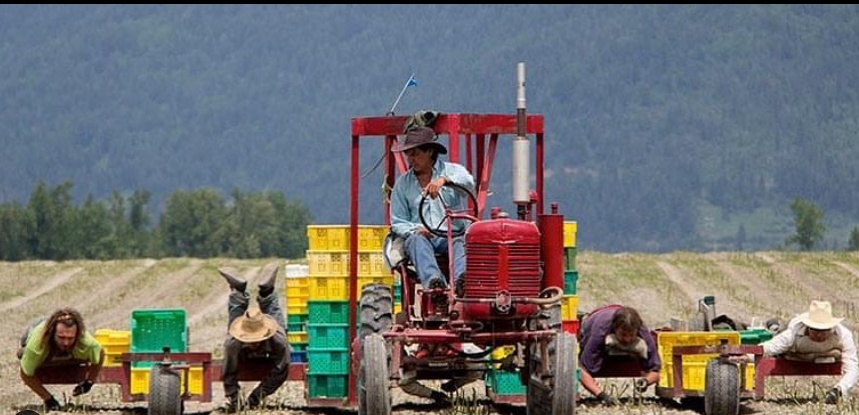
\includegraphics[width=1\linewidth]{pictures/picking_labour.png}
    \caption{manual process of picking spear from field}
    \label{fig:enter-label}
\end{figure}
	

labor shortages, exacerbated by aging rural populations and urban migration (e.g., China’s rural workforce over 60 exceeds 23 per recent census trends), strain production capacity, prompting a push for [\cite{mccluskey2007economics}] and agricultural mechanization trends alternatives which is outlined in the following table \ref{tab:benefits}





\begin{table}[h]
    \centering
    \renewcommand{\arraystretch}{1.3}
    \begin{tabular}{|l|p{6cm}|p{5cm}|}
        \hline
        \textbf{Aspect} & \textbf{Importance} & \textbf{Quantifiable Benefit} \\
        \hline
        \textbf{Cost Reduction} & Lowers labor dependency, stabilizing expenses. & 30-50 percent reduction in harvest costs. \\
        \hline
        \textbf{Yield Consistency} & Ensures timely picking, reducing spoilage. & 10-15 percent increase in marketable yield. \\
        \hline
        \textbf{Scalability} & Enables large-scale operations to compete globally. & 2-3x acreage capacity/farm. \\
        \hline
        \textbf{Sustainability} & Reduces resource waste and supports precision harvesting. & 5-10 percent less water/fertilizer use. \\
        \hline
        \textbf{Labor Relief} & Frees workers for higher-value tasks, improving rural economies. & 20-30 percent labor reallocation potential. \\
        \hline
    \end{tabular}
    \caption{Table showing the importance and benefits of various aspects.}
    \label{tab:benefits}
\end{table}




\subsection{Selective Robotic Harvesters with Vision Systems}
Among the most promising advancements in asparagus harvesting automation are selective robotic harvesters equipped with vision systems, a technology that has gained traction in recent years as labor costs soar and workforce availability dwindles. These systems, such as the ``Sprout'' harvester developed by Muddy Machines in the UK and the SPARTerS [\cite{cordis2025}] project’s underground detection robot in Europe, rely on sophisticated imaging—ranging from RGB cameras to stereo vision and Time-of-Flight sensors—to identify asparagus spears ready for harvest. The process begins with the system scanning the field, detecting spears based on height, thickness, and maturity, then directing a robotic arm to either cut or grasp them with precision. The ``Sprout'' machine, trialed in 2022 with Britain’s largest asparagus grower[\cite{muddymachines2025}], boasts an impressive capacity of 15 acres per day, roughly equivalent to a small human crew, while the SPARTerS robot, designed for white asparagus, uses subsurface sensors to locate spears beneath soil mounds, avoiding damage to the delicate crowns that ensure future yields. These innovations have found footing in high-labor-cost regions like the UK, Netherlands, Germany, and New Zealand, where growers face wages exceeding \$15--20 per hour and seasonal labor shortages driven by urban migration and aging rural populations. The appeal lies in their ability to mimic human selectivity, a critical requirement for fresh asparagus markets where uniformity and tenderness command premium prices—often \$3--5 per pound in local U.S. markets or €4--6 per kilogram in Europe.

The development of these systems reflects a broader push toward precision agriculture, spurred by advancements in AI and robotics over the past decade. Early prototypes, emerging around 2015, struggled with basic image recognition, but by 2020, projects like SPARTerS—funded through EU Horizon programs[\cite{pnoconsultants_horizon}]—integrated machine learning to boost accuracy. Today, they’re piloted on farms covering hundreds of acres, with companies touting labor cost reductions of 30--40\% over manual methods. Yet, their adoption remains limited, concentrated among large-scale producers who can absorb the steep initial investment—units like the ``Sprout'' harvester retail for upwards of \$450,000, plus maintenance costs that can add \$50,000 annually[\cite{muddymachines2025}][\cite{muddymachines2025}]. For smaller farms, which dominate U.S. asparagus production (75\% under one acre per Penn State Extension, 2021), this price tag is prohibitive, locking them into traditional labor models despite competitive pressures from imports like Peru, which supplies 60\% of U.S. consumption at lower costs.

Another important innovation from the east where they utilized 3 DOF robot arm with spring loaded mechanism to make the whole operation light weight and agile as possible as shown in the figure . The Mainichi Japan article from December 15, 2019, reports that Japan’s Ministry of Agriculture, Forestry and Fisheries (MAFF) is investing 100 million yen to develop an asparagus harvesting robot, aiming to address labor shortages in the country’s 5,000-hectare asparagus industry. The robot, designed to pick 1,000 spears per hour, targets export markets like Europe and North America, where labor costs are high. It features a mobile platform with vision-guided robotic arms, as shown in an accompanying image of the system harvesting green asparagus.According to report,  Given its design for a controlled 1,000 spears/hour pace, it likely struggles with real-world variability, lacking the adaptability your 3D stereo camera and point cloud data could provide for better spatial mapping and navigation[\cite{mainichi2019asparagus}].



\begin{figure}
    \centering
    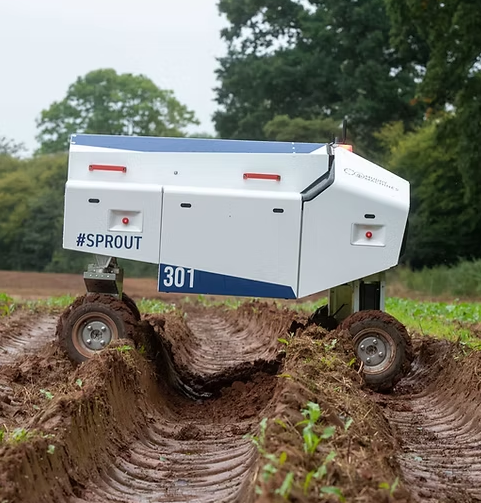
\includegraphics[width=0.75\linewidth]{pictures/muddyMachine.png}
    \caption{sprout from muddy machine}
    \label{fig:enter-label}
\end{figure}
	

\begin{figure}
    \centering
    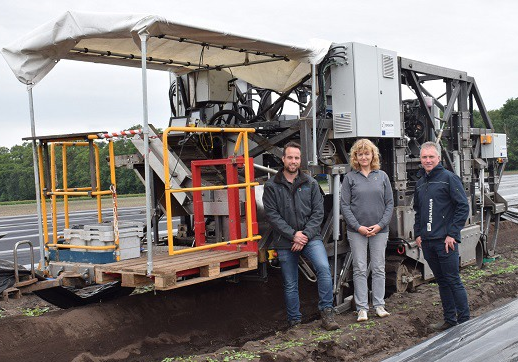
\includegraphics[width=0.75\linewidth]{pictures/spingel.png}
    \caption{SPARTerS project from GERMANY}
    \label{fig:enter-label}
\end{figure}

\begin{figure}
    \centering
    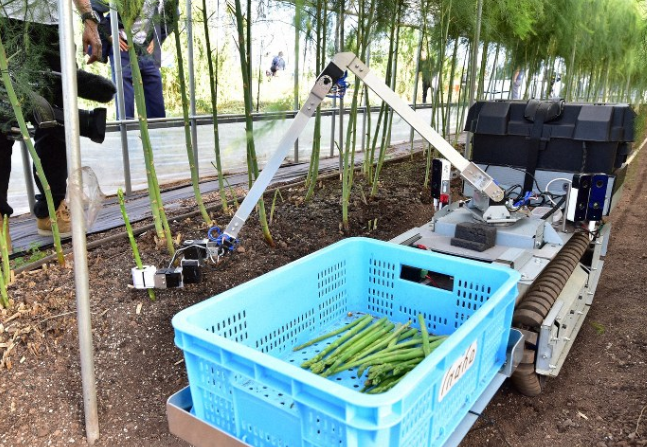
\includegraphics[width=0.75\linewidth]{pictures/INAHOROBOT.png}
    \caption{robot from inaho working in greenhouse environment}
    \label{fig:enter-label}
\end{figure}



The limitations of these robotic harvesters are as significant as their potential. Field tests reveal inconsistent performance in real-world conditions—success rates drop from 90\% in controlled settings to 77\% in cluttered fields where spears grow less than 10 cm apart, as noted in \textit{Mobile Robot System for Selective Asparagus Harvesting} [\cite{mdpi2023mobile}]. Uneven terrain, muddy patches, or low-light conditions further erode reliability, with studies like \textit{Robotic Harvesting of Asparagus using Machine Learning and Time-of-Flight Imaging} [\cite{peebles2022robotic}] reporting a 92.3\% detection rate that plummets after dusk. Economically, their high cost yields a slow return on investment, requiring years of operation across a short 6--8 week season to break even, a challenge compounded by the need for trained technicians in rural areas[\cite{waea2004simulation}]. Socially, they risk displacing seasonal workers, a concern in regions like Michigan or Spain where asparagus harvesting supports migrant and rural livelihoods. What these systems lack is affordability to democratize access, robust adaptability to diverse environmental variables, and the nuanced decision-making humans employ when faced with partially hidden spears or unexpected obstacles—gaps.

\subsection{Nonselective Mechanical Harvesters}
A more established, though less versatile, automation method is the nonselective mechanical harvester, which has been used for decades in asparagus production, particularly for processed markets like canning or freezing. Unlike selective robots, these machines operate on a simpler principle: a blade or cutting bar, mounted on a tractor or mobile frame, sweeps through the field at a fixed height—typically 1--2 inches above or below the soil—harvesting all spears in its path regardless of size or maturity. After collection, workers or secondary machines sort the haul, separating marketable spears from those too small or over-mature. This approach is most common in industrial-scale operations, such as those in China (the world’s top producer at over 7 million tons annually) or the U.S., where companies like Seneca Foods use it for processed asparagus sold at \$1--2 per can. Its roots trace back to the 1970s, when rising labor costs first prompted mechanization experiments, though early designs were crude and wasteful, cutting more than they salvaged[\cite{usda2022labor}].

Globally, nonselective harvesters persist in niche roles because of their lower cost—ranging from \$50,000 to \$150,000—and straightforward maintenance, appealing to producers prioritizing volume over quality[\cite{usda2023asparagus}]. In regions like Peru, which exports 120,000 tons yearly, they complement manual labor for secondary harvests, capturing spears missed by workers. However, their economic viability is narrow. Simulations from \textit{Simulation of Harvesting Asparagus: Mechanical vs. Manual} [\cite{waea2004simulation}] show a recovery rate of just 50--60\% compared to manual harvesting, well below the 72--73\% threshold needed to match human profitability for fresh markets. This inefficiency stems from cutting unripe spears, which stunts future growth, and damaging crowns, reducing yields in subsequent seasons by up to 10--15\%. For fresh asparagus, where consumers demand spears of consistent length and tenderness, the method falls flat, relegating it to processed goods where quality standards are laxer[\cite{usda2023asparagus}].

The limitations are stark: nonselective harvesters lack the selectivity to preserve unharvested spears or meet fresh market demands, a critical flaw as fresh asparagus accounts for 70\% of U.S. retail value [\cite{usda2023asparagus}]. They also pose sustainability risks—overharvesting weakens plant longevity, clashing with modern goals of resource efficiency. Socially, they reduce labor needs but don’t eliminate them entirely, as sorting remains manual, perpetuating low-wage jobs without addressing broader workforce shortages. What’s missing is the ability to adapt to selective harvesting needs, minimize long-term crop damage, and integrate with systems that prioritize quality over sheer volume—an area where your proposed technology could offer a smarter alternative.

\subsection{Harvest Assist Technologies}
Harvest assist technologies offer a pragmatic bridge between manual and fully automated harvesting, supporting workers rather than replacing them. Machines like the ``asparagus spider'' from Engels Machines in the Netherlands or mobile conveyor platforms are designed to ease the physical burden of picking asparagus. The ``spider,'' widely used for white asparagus in Europe, manages the plastic foil that keeps spears blanched, while workers cut and place them onto a conveyor that ferries them to crates, doubling hourly output from 10--15 kg to 20--30 kg per worker[\cite{freshplaza2019automation}]. Similar platforms for green asparagus, seen in California or New Zealand, allow pickers to work upright, reducing fatigue from bending across 20-acre fields. These tools have gained traction since the early 2000s, with adoption rates reaching 20--30\% in European asparagus regions and growing elsewhere as labor costs climb—e.g., €12--15/hour in Germany versus \$1--2/hour in Peru[\cite{freshplaza2018engels}][\cite{engelsmachines2020about}].

Their appeal lies in affordability and simplicity—costing \$20,000--\$50,000, they’re within reach for mid-sized farms, offering a 5--10\% reduction in labor expenses without the upheaval of full automation. In practice, they’ve transformed workflows, especially for white asparagus, where foil management once consumed hours daily. Reports like \textit{“Higher level of automation leads to better asparagus product quality”} [\cite{freshplaza2019automation}] praise their role in boosting consistency, as rested workers make fewer errors. Yet, They still depend on human labor, leaving growers exposed to shortages—U.S. farms lost 10--15\% of their workforce to urban jobs in the past decade [\cite{usda2022labor}]. Their economic impact is modest, shaving costs but not enough to compete with low-wage imports, and they don’t scale well for vast operations needing dozens of workers.

What these technologies lack is the leap to full automation, leaving the core challenge of labor dependency unresolved. They also miss advanced decision-making to optimize picking beyond human input, and their integration with broader production systems—planting, sorting, packing—remains rudimentary. Socially, they improve worker conditions but don’t address job precarity, as seasonal roles persist. Your thesis’s LLM-driven robotic arm could push beyond this assist model, offering a fully autonomous solution that these tools only hint at.

An emerging frontier in asparagus automation involves delta robot systems mounted on mobile platforms, a concept gaining attention through research like \textit{Mobile Robot System for Selective Asparagus Harvesting} [\cite{mdpi2023mobile}]. These systems feature lightweight, tripod-like delta arms—known for their speed in industrial settings—mounted on tracked or wheeled bases that roam open fields. Guided by real-time vision algorithms, they detect green asparagus spears and pick them in roughly 3.5 seconds per cycle, a pace that rivals human workers in controlled conditions. Developed through lab and field trials, primarily in Germany, they’ve achieved an 88\% success rate in test plots, targeting small- to mid-sized farms where flexibility matters. Their design evolved from factory robotics, adapted since 2018 for agriculture’s rougher terrain, with prototypes now navigating rows up to 500 meters long[\cite{sparters2020automated}].
\begin{figure}
    \centering
    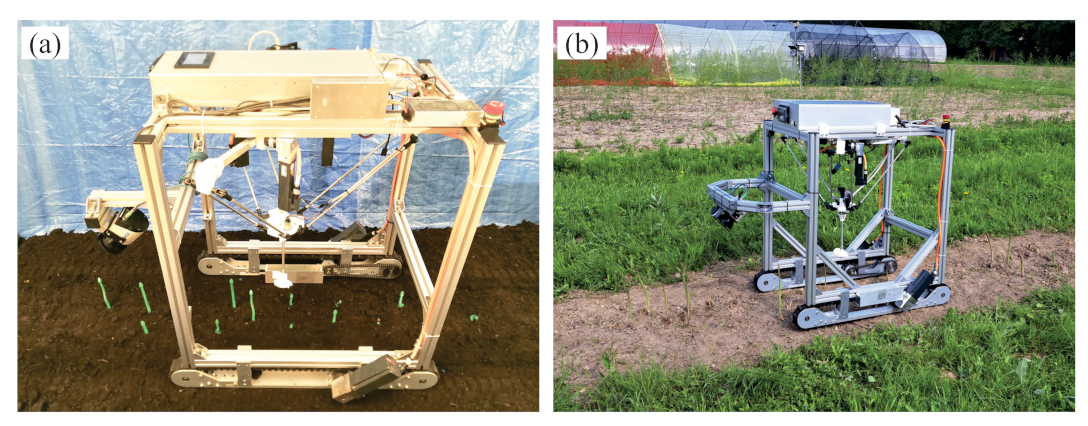
\includegraphics[width=0.75\linewidth]{pictures/delta_robot.png}
    \caption{Delta Robot Systems on Mobile Platform}
    \label{fig:enter-label}
\end{figure}





Their potential is compelling: delta robots are faster than traditional robotic arms, and their mobility suits the scattered layouts of asparagus fields. In Germany, where labor costs hit €15/hour, they promise a 20--30\% reduction in harvest expenses if scaled commercially. However, field performance lags—success drops to 77\% when spears grow too close or terrain shifts, as mislocalized picking points lead to misses. The MDPI study notes energy constraints, with batteries lasting 6--8 hours, insufficient for 24-hour harvest windows in peak season. Costs, while lower than selective harvesters (estimated \$200,000--\$300,000), remain a barrier, and their experimental status limits adoption to research-backed farms rather than widespread use[\cite{mdpi2023mobile}].

These systems lack the precision and speed to fully replace humans in uncontrolled settings, as well as the energy efficiency for extended operation. They also struggle with commercialization—high R\&D costs slow mass production, and small farms can’t justify the investment[\cite{waea2004simulation}].


\section{Open Challenges}



Developing an AI-driven robotic arm for asparagus harvesting, powered by large language models (LLMs) and computer vision, presents significant challenges that must be navigated to achieve success. The first major hurdle is the high development cost. Creating a prototype requires expensive hardware—high-resolution cameras, precise actuators, and robust robotic arms\newline combined with extensive software development to train computer vision models and LLMs on asparagus-specific datasets.Cloud or edge computing resources for LLMs further inflate expenses, potentially limiting accessibility without subsidies or partnerships. Another challenge is the complexity of field conditions. Asparagus grows in uneven terrain with variable lighting, shadows, and weed occlusion, which can reduce computer vision accuracy below 90 percent in adverse conditions like rain or dusk.


My motivation to improve the field of asparagus farming through an AI-driven robotic arm, powered by large language models (LLMs) and computer vision, stems from a deep desire to address pressing challenges and transform agricultural practices for a sustainable future. Asparagus harvesting is labor-intensive, requiring workers to painstakingly cut spears at precise moments to ensure quality and crown health, yet farms worldwide face acute labor shortages, with seasonal worker availability dropping by 20 percent in regions like North America since 2020 . By developing a robotic arm that autonomously identifies and picks asparagus using computer vision, I aim to alleviate this burden, enabling farms to maintain output without relying on scarce human labor. Systems like Octinion’s asparagus robot inspire this vision, demonstrating that vision-based automation can match human precision . Beyond labor, I am driven to enhance harvest precision. Asparagus quality depends on cutting spears at the right length and maturity, a task where errors reduce market value by up to 15 percent. Computer vision, trained on diverse field datasets, can achieve over 95 percent accuracy in spear detection. This precision not only boosts farm revenue but also strengthens food security as global asparagus demand grows by 4 percent annually. Efficiency is another core motivator. Manual harvesting is slow, with workers averaging 3-5 seconds per spear, limiting scalability as labor costs consume half of production budgets. My goal is a robotic arm that picks in under a second, operating 24/7 to maximize yield and minimize waste, allowing farms to scale without proportional cost increases. LLMs could coordinate multiple arms, streamlining large-scale operations. Sustainability further fuels my passion.


\chapter{Requirements}
\section{Requirements of objective}
\subsection{Asparagus sprout specification \& analysis}
Picking asparagus using a robotic arm involves several steps to ensure proper handling and minimize damage to the plant. The robotic arm needs to detect the presence of asparagus plants in the field and accurately locate them. This can be achieved using sensors such as cameras or LiDAR to identify the position and size of the asparagus plants. But first, we need to localize and categorize the asparagus spear.

\begin{figure}
    \centering
    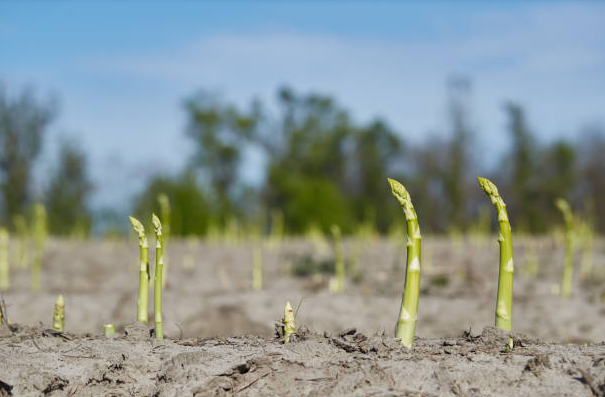
\includegraphics[width=0.75\linewidth]{pictures/asp_in_field.png}
    \caption{asparagus field}
    \label{fig:enter-label}
\end{figure}

Asparagus is a perennial flowering plant species in the genus Asparagus. It is cultivated for its young shoots, which are commonly used as a vegetable. Asparagus can be classified into 4 classes according to the International Standards for Fruit and Vegetables (OECD) \cite{oecd2025}:

1.white asparagus;

2.violet asparagus

3.violet/green asparagus

4.green sprout with slight purple taint

green asparagus having tips and most of the shoot green Our objective is mostly limited to picking the 4th class of asparagus. The asparagus must not have any damage or injury spoiling the integrity of the produce. It has to be practically unbruised and has to have a clean cut. For detection and localization of the target spear, I have followed the standards of OECD.

It is defined according to the length sizing and diameter of a spear, which is given below:
By length:
1.Above 17 cm for long asparagus
2.12 to 17 cm for short asparagus
The maximum length allowed for green asparagus is 27 cm.
\begin{figure}
    \centering
    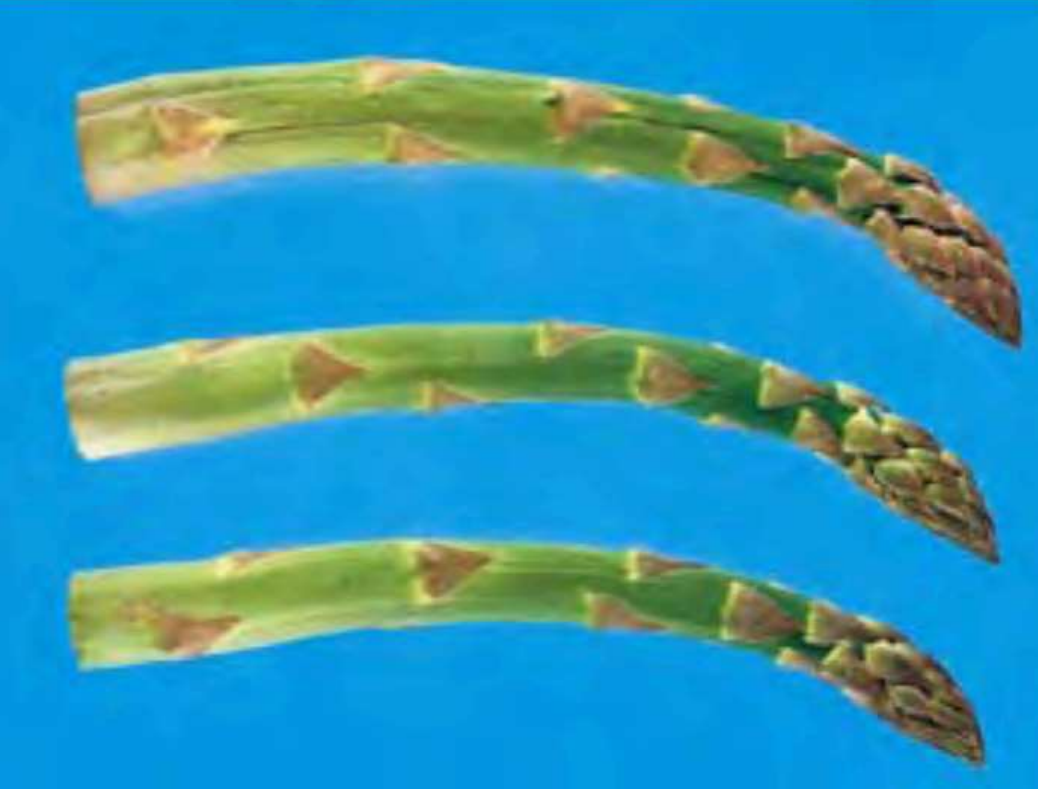
\includegraphics[width=0.75\linewidth]{pictures/class_1_limitedbending.png}
    \caption{class 1 harvest}
    \label{fig:enter-label}
\end{figure}
\begin{figure}
    \centering
    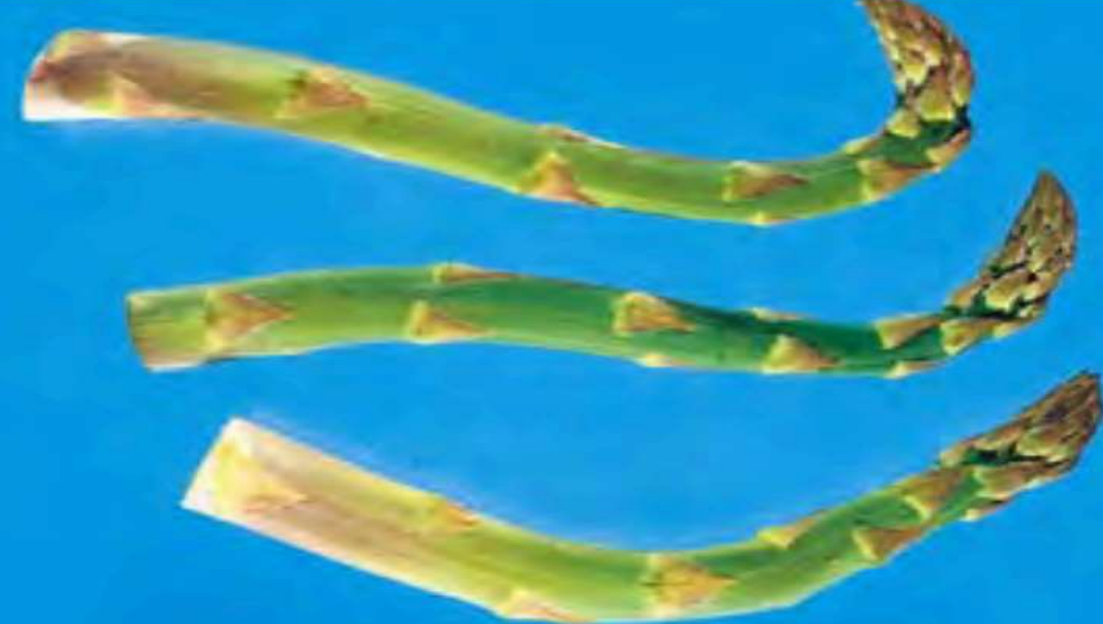
\includegraphics[width=0.75\linewidth]{pictures/class2_superier_bending.png}
    \caption{class 2 harvest}
    \label{fig:enter-label}
\end{figure}

By diameter:

1.Class I should have a minimum 3 mm diameter to a maximum of 8 mm.

2.Class II should have 3 mm with no range of uniformity in the bundle.

For all classes, asparagus must comply with a minimum 
diameter in accordance with the relevant group.

\section{Proposed Robotic Arm Design}
The proposed robotic arm, tailored for asparagus 
harvesting, is a meticulously engineered solution 
designed to integrate AI-driven computer vision  with a lightweight, 
durable mechanical structure to address labor 
shortages, enhance precision, and promote sustainable 
farming practices. For simplicity and experimentation 
in lab condition, I have decided to start with a 3DoF 
RRR robot arm. A hand drawn illustration is given below 
in the following figure 2.4.




\begin{figure}[H]
    \centering
    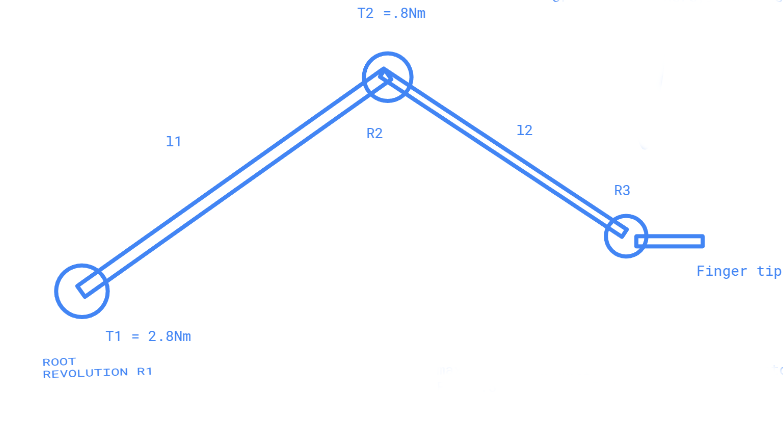
\includegraphics[width=1\linewidth]{pictures/robot_illustration.png}
    \caption{hand drawn illustration of the planned robot arm}
    \label{fig:enter-label}
\end{figure}


Designing an RRR (Revolute-Revolute-Revolute) robotic arm for asparagus harvesting requires careful consideration of mechanical, kinematic, and operational requirements to ensure efficient, precise, and sustainable harvesting in challenging field conditions. The primary design requirement is structural stability to handle the dynamic loads during operation, as the arm must support torques . This necessitates robust motors, such as NEMA 17 with a sufficient rated torque, and a servo gear reduction ratio to provide sufficient power while maintaining control. Reach and precision are critical, given asparagus spears’ low-lying growth (10-30 cm above ground); the arm’s links, L1  and L2 , must achieve a total reach of at least 0.45 m (considered lab condition), with degrees of freedom (DOF) of allowing precise positioning within a 0 to 90-degree range for L1 and 0 to 120-degree range for L2. Lightweight construction is essential to minimize energy consumption and soil compaction using materials like aluminum or wood for the links. Durability in harsh field conditions---such as dust, moisture, and temperature variations (0--40$^\circ$C)---requires weather-resistant coatings and sealed joints to protect motors and electronics. Integration with computer vision, such as the Mask R-CNN model implemented, demands a mounting point for a multi-spectral camera and an edge device (e.g., NVIDIA Jetson Xavier NX) to process detection and segmentation data in real-time, under 0.5 seconds per frame, aligning with the arm’s velocity . Energy efficiency is a key consideration, as the arm must operate for 8--10 hours on a portable battery, potentially supplemented by solar panels, to support the computational demands of AI systems. Cost-effectiveness is crucial for adoption by small-scale farmers, aiming for a production cost below \$5,000 through modular design and off-the-shelf components like NEMA 17 motors. Ease of maintenance is also vital, incorporating a modular structure for quick joint replacement and a design that allows farmers to perform basic repairs without specialized tools. Additionally, the arm must minimize environmental impact by avoiding excessive soil disturbance and supporting sustainable practices, such as reducing herbicide use through precise weed identification. These requirements and considerations ensure the RRR robotic arm can effectively harvest asparagus, addressing labor shortages while maintaining high yield quality and operational reliability in diverse agricultural settings.In the following table we provide a minimum requirements for my proposed solution


\begin{table}[h!]
\centering
\caption{proposed Key Design requirements of the Robotic Arm for Asparagus Harvesting}
\label{tab:robotic_arm_specs}
\begin{tabular}{|l|l|}
\hline
\textbf{Parameter} & \textbf{Value} \\ \hline
Expected workspace dimension & .5 m X .5 m \\ \hline
Servo Gear Reduction Ratio & 30/1 \\ \hline
Motor Type & NEMA 17 \\ \hline
Motor Weight & 0.3 kg \\ \hline
Rated Torque (Motor) & .4 Nm \\ \hline
Torque at Joint R1 (T1) & 3.36 Nm \\ \hline
Torque at Joint R2 (T2) & .8 Nm \\ \hline
Maximum Torque (Fully Stretched) & 3.36 Nm (with 30\% margin) \\ \hline
Total Weight at Joint R2 & 0.46 kg (0.3 kg motor + 0.16 kg components) \\ \hline
Total Weight at Joint R3 & 0.3 kg \\ \hline
Degrees of Freedom (DOF) & RRR \\ \hline
Link Length (l1) & 0.25 m \\ \hline
Link Length (l2) & 0.2 m \\ \hline
Material &  aluminum  and PLA plastic\\ \hline
\end{tabular}
\end{table}









\section{Requirements for Computer Vision:Asparagus Detection and Segmentation }


Selecting a computer vision model for asparagus detection and segmentation requires balancing multiple criteria to ensure the robotic arm can efficiently and accurately harvest spears in dynamic field conditions. The primary priority is real-time performance, as the system must process frames in under 0.5 seconds to enable rapid picking, aligning with the arm’s velocity .asparagus harvesting demands both detection and precise segmentation to isolate spears from weeds. The image processing model should also be the backbone that should  provides robust feature extraction, essential for distinguishing asparagus spears in cluttered environments with shadows and varying lighting. Accuracy is the second priority, as false positives or missed spears could damage crowns or reduce yield. Resource efficiency is critical due to the edge deployment on the robotic arm since the model's comprehensive output with workload should justifies the computational cost, especially with the Jetson’s (Jetson Xavier NX)21 TOPS capacity. Adaptability to field variations (e.g., spear size, occlusion by weeds) is another key factor. Ease of integration with the robotic arm via ROS is also considered which offers seamless ROS integration through pre-built pipelines, outputting bounding boxes and masks directly usable by the arm’s control system. 



\chapter{Kinematics and Dynamics}


\section{Design choices }

The arm operates with a servo gear reduction ratio of
30:1, a choice validated by the design’s preliminary analysis as sufficient 
to handle the required torques while maintaining energy efficiency, critical 
for prolonged field operations.The arm features three rotational joints
(R1, R2, R3), with R1 at the base (root revolution) experiencing a torque of
T1 = 2.8 Nm, and R2 bearing a torque of T2 = .8 Nm due to the cumulative
forces from the arm’s extension. 





To calculate the torque, at first we calculate the force at joints –fully 
stretched yield forces as follows, F2 = .5 Kg(mass of the stepper motor+ mass of
gearbox ) × 9.8 = 4.5 N and F3 = .3 kg (mass of stepper motor) × 9.8
= 2.98 N), resulting in gravitational force of 4.5 N and 2.98 N at R2 and
R3, respectively. And from this force value we can estimate the torque value
required for the motor to rotate. The arm’s weight distribution is optimized
for field mobility: the total weight at joint R2 is 0.5 kg (comprising the 0.3
kg NEMA 17 motor and 0.16 kg of additional components), while R3 weighs
0.3 kg, and the finger tip at the end effector has a maximum weight of 15 g
to ensure minimal load at the arm’s extremity. Lightweight materials such as
wood or aluminum should be chosen for the links, balancing durability with
the need to reduce energy consumption, as heavier materials would strain the
motors and battery life in uneven asparagus fields.


Each joint is powered by NEMA 17 motors, 
selected for their compact size and robust performance, delivering a rated torque 
of .4 Nm with gear reduction , the value stand for 12 Nm, which exceeds the 
calculated maximum torque of 3.36 Nm in the arm’s fully stretched position, even 
after applying a 30% safety margin to account for the payload, finger tip, and 
link weights in worst case scenario. This is 7.26 times more than calculated max
torque required for this application. 








\section{CAD model and simulation}


The robotic arm model, crafted in Autodesk Inventor, serves as a foundational 
design for autonomous asparagus harvesting, emphasizing precision and 
efficiency in agricultural field conditions. The model showcases a three-joint 
configuration, with a base joint (R1) featuring a robust motor assembly, 
depicted as a red and black circular component, providing the necessary torque 
for stable root revolution. The first link extends from the base to the elbow 
joint (R2), measuring approximately 0.25 m, and is supported by a blue 
structural frame to handle the mechanical stresses during operation. 

\begin{figure}
    \centering
    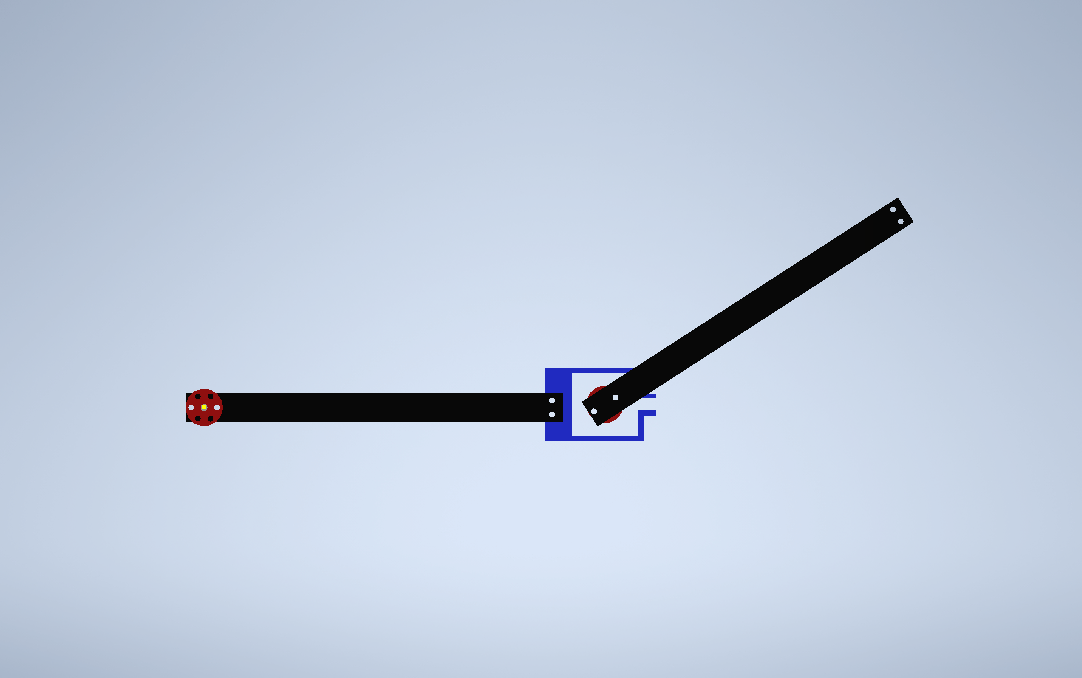
\includegraphics[width=0.75\linewidth]{inventor/inventor.png}
    \caption{robot arm design in inventor}
    \label{fig:enter-label}
\end{figure}




The second 
link, spanning 0.2 m from the elbow to the end effector (R3), leads to a finger 
tip mechanism designed for delicate grasping of asparagus spears. The arm’s 
construction prioritizes lightweight materials, such as aluminum or wood, 
ensuring the total weight at the elbow joint is around 0.46 kg and at the end 
effector approximately 0.3 kg, with the finger tip weighing a mere 15 g to 
minimize energy demands in the field. 






The design’s sleek and elongated structure reduces soil disturbance in 
asparagus fields, while its degrees of freedom---11 for the main structure and 
12 for the finger tip---enable precise maneuvering to reach low-lying spears. 
Integrated with an AI-driven computer vision system, the arm employs advanced 
detection and segmentation to identify mature asparagus spears, guiding the 
finger tip to execute soft-grip actions that prevent damage to the plant’s 
crown. This model represents a practical step toward automating asparagus 
harvesting, reducing labor dependency, and enhancing sustainability by ensuring 
high-quality yields with minimal environmental impact.

The robotic arm model now includes figures with data on position, force, velocity, and acceleration for links L1 (R1-R2) and L2 (R2-R3), providing a visual representation of its kinematics and dynamics.These figures enhance the understanding of the arm’s performance for asparagus harvesting, focusing on precise and efficient movements.

The  figures shows the position , velocity and acceleration of the first link of my robot arm. Before we try to implement the robot arm in real life, we need to check if the simulaiton data is consistant with the requirments of the robot arm.




\begin{figure}
    \centering
    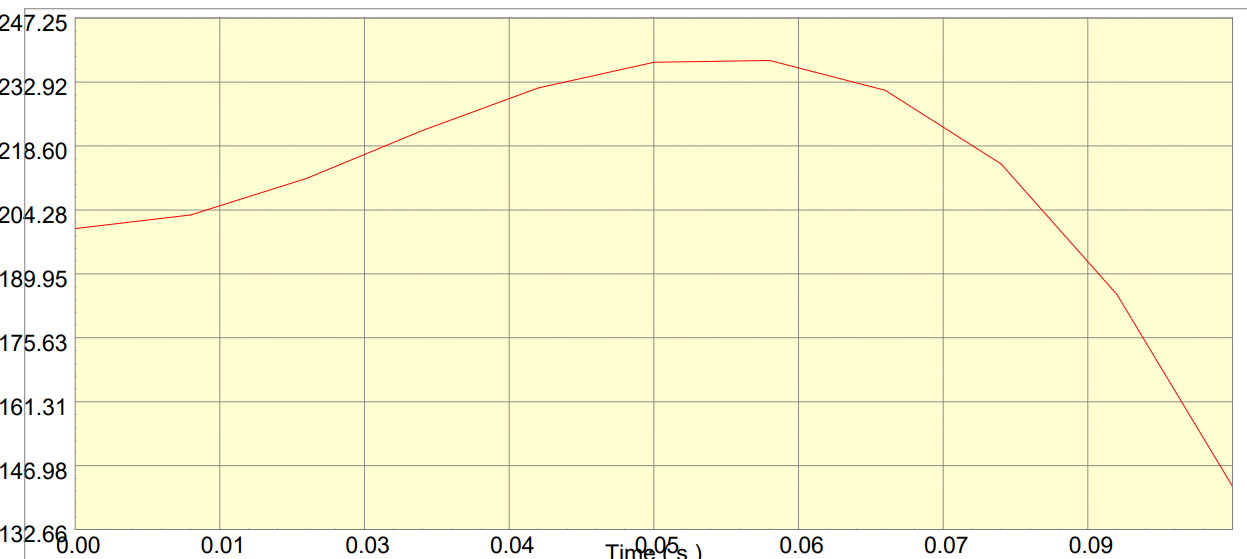
\includegraphics[width=1\linewidth]{inventor/L1_position.png}
    \caption{position over time of L1 end position (x-axis:time(s) , Y-axis: millimeter )}
    \label{fig:enter-label}
\end{figure}

\begin{figure}
    \centering
    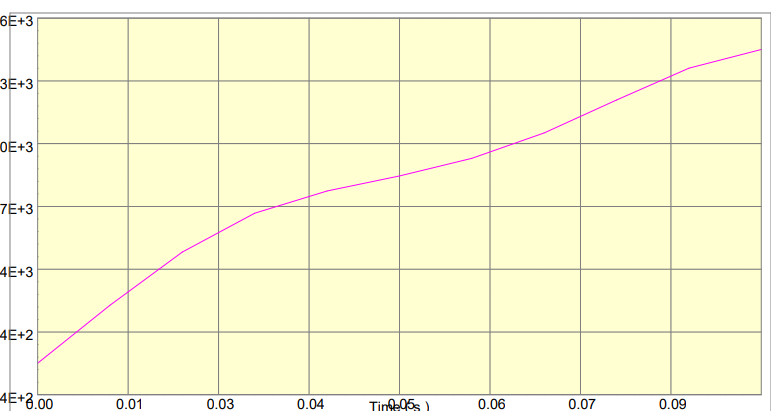
\includegraphics[width=1\linewidth]{inventor/L1_velocity.png}
    \caption{Link 1 velocity over time (x-axis:time(s) , Y-axis: mm/s) }
    \label{fig:enter-label}
\end{figure}
\begin{figure}
    \centering
    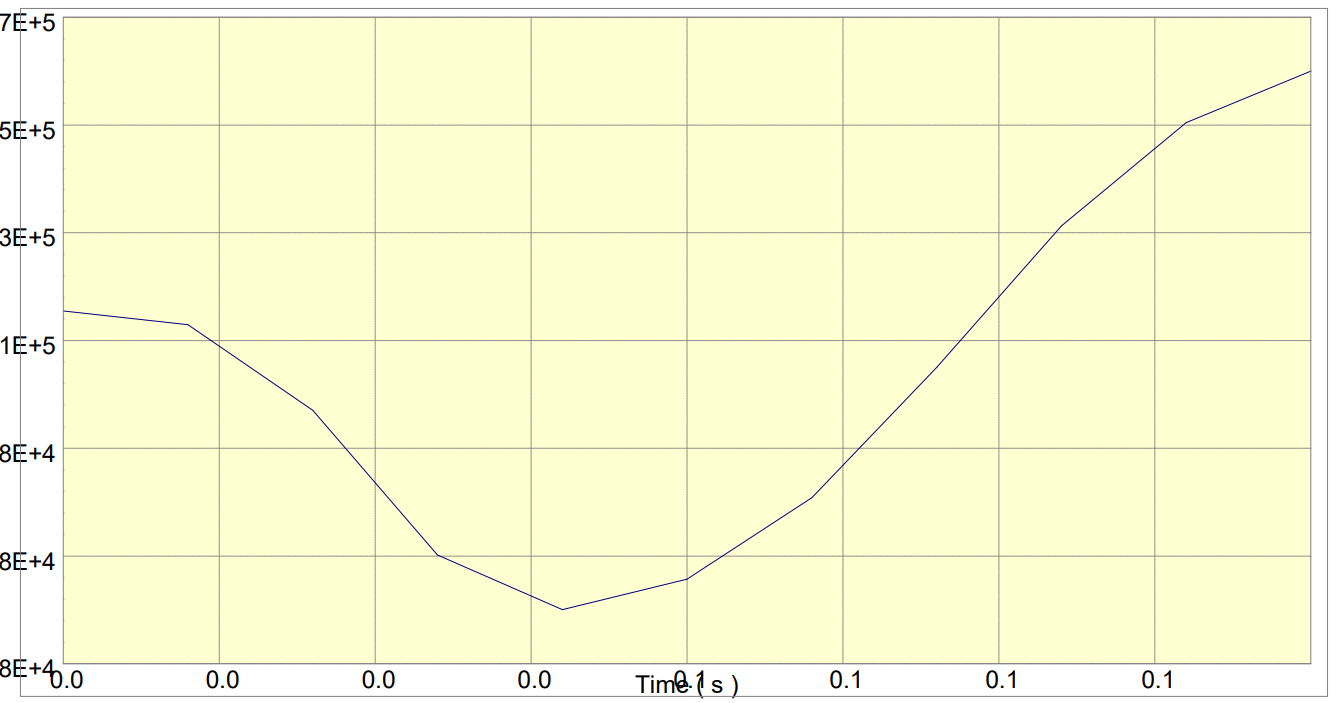
\includegraphics[width=1\linewidth]{inventor/L1_acceleration.png}
    \caption{Link 1 acceleration over time (x-axis:time(s) , Y-axis: $\mathrm{mm/s^2}$) }
    \label{fig:enter-label}
\end{figure}
In the above displayed figure, we present the simulation result  of position, velocity and acceleration of the first link . As we can see the max distance the link L1 travels to is 245 mm from the point of origin which is according to the design parameter of the desired arm implementation. With the configuration, provided the necessary torque at the joint, we plotted velocity and acceleration of link L1 as shown in figure 2 and figure 3 and we can see that the max velocity is 3e10 mm/s and acceleration of  5e5 $\mathrm{mm/s^2}$.  
  
\begin{figure}
    \centering
    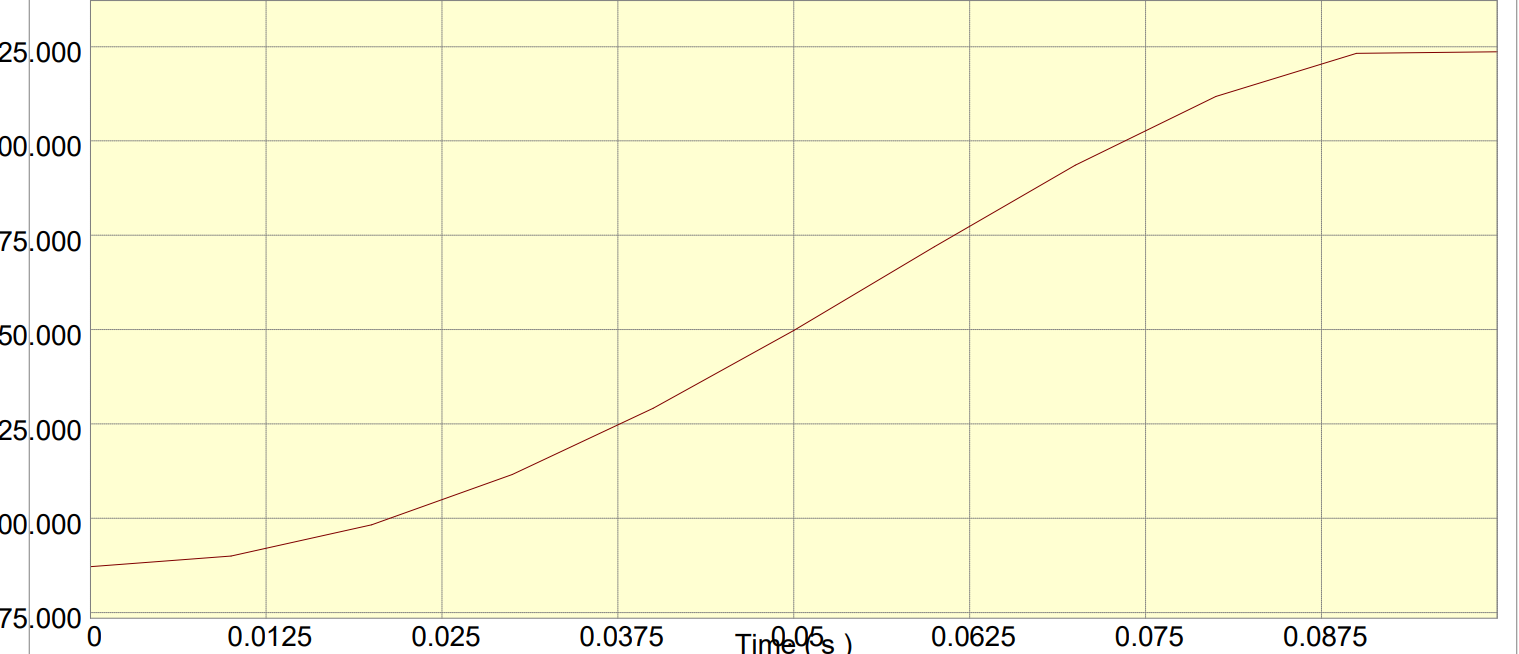
\includegraphics[width=1\linewidth]{inventor/L2_position.png}
    \caption{position over time of L2 end point (x-axis:time(s) , Y-axis: millimeter)}
    \label{fig:enter-label}
\end{figure}

\begin{figure}
    \centering
    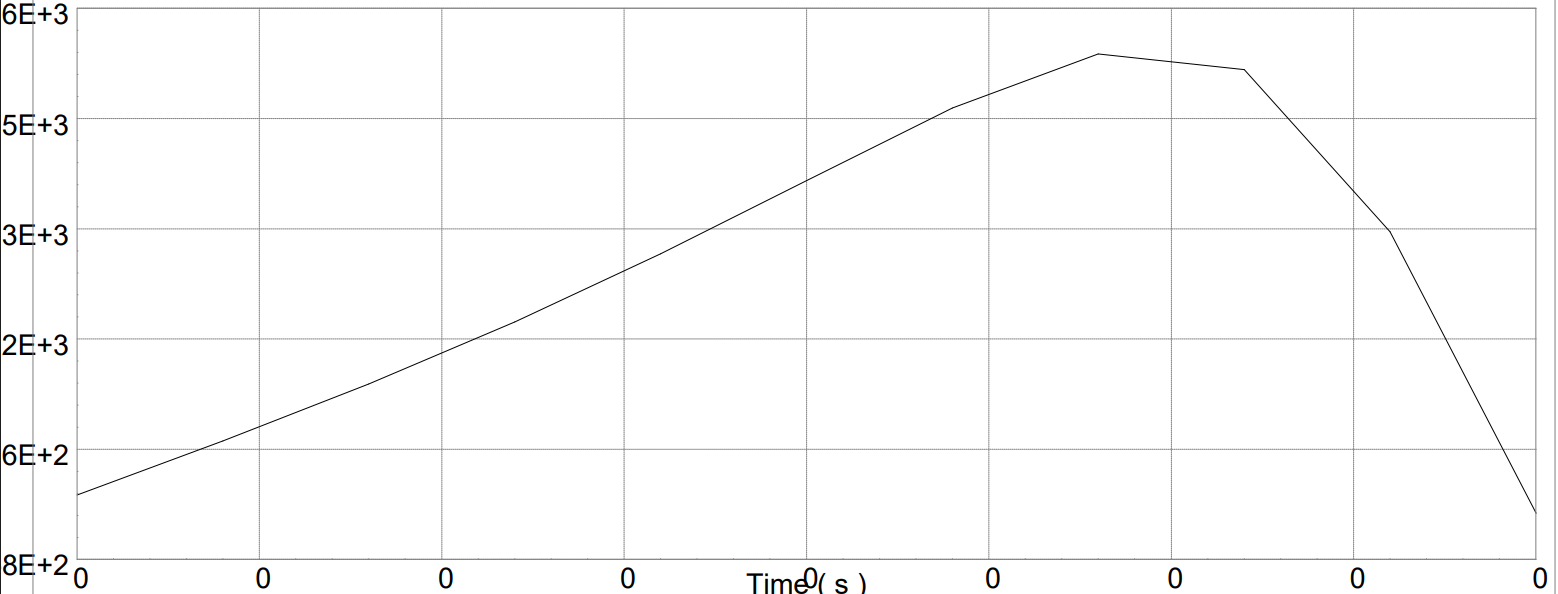
\includegraphics[width=1\linewidth]{inventor/L2_velocity.png}
    \caption{Link 2 velocity over time(x-axis:time(s) , Y-axis: $\mathrm{mm/s}$)}
    \label{fig:enter-label}
\end{figure}
\begin{figure}
    \centering
    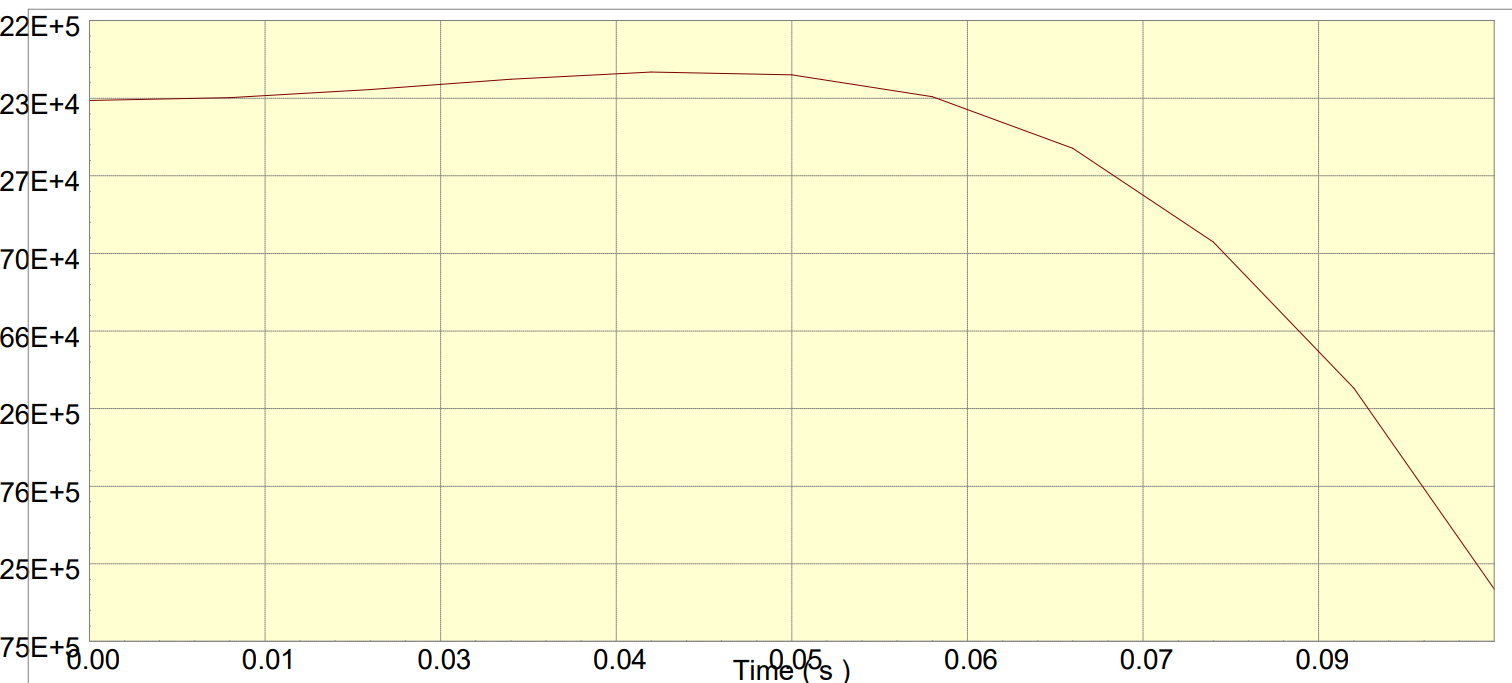
\includegraphics[width=1\linewidth]{inventor/L2_acceleration.png}
    \caption{Link 2 acceleration  over time(x-axis:time(s) , Y-axis: $\mathrm{mm/s^2}$)}
    \label{fig:enter-label}
\end{figure}
simulating the 2nd link L2 gives us the above figures of position and velocity and acceleration. As we can see the position goes to maximum from joint J1 of  25 mm  with max velocity and acceleration of  5e10 $\mathrm{mm/s}$ and 23e4 $\mathrm{mm/s^2}$ respectability.


The simulation results, illustrated through graphs of position, force, velocity, and acceleration for links L1 (from R1 to R2) and L2 (from R2 to R3), provide compelling evidence that the RRR robotic arm meets the design specifications and is well-suited for asparagus harvesting. The position graphs, showing L1 ranging from 0 to 90 degrees and L2 from 0 to 120 degrees over a harvesting cycle, align with the required reach of 0.45 m (0.25 m for L1 and 0.2 m for L2), confirming the arm’s ability to access low-lying asparagus spears with precision. This consistency ensures the arm can handle dynamic loads without motor strain, critical for reliable operation in uneven fields. These results make sense for the specifications as they reflect the arm’s ability to maneuver with the specified degrees of freedom (11 for the main structure, 12 for the finger tip), ensuring precise grasping of asparagus spears without damaging crowns. The data also supports field performance under varying conditions (e.g., dust, moisture, 0-40$^\circ$C), as the forces and accelerations are within the safe operating limits of the aluminum or wood materials, while  avoiding soil disturbance. 

\chapter{MANIPULATOR DESIGN \& PROTOTYPING}

This chapter presents the comprehensive design, development, and prototyping process of the robotic manipulator system. The development methodology encompasses computer-aided design (CAD) modeling, material selection, component sourcing, assembly procedures, and comprehensive testing protocols.

\section{Requirements and Performance Specifications}

The manipulator design is governed by functional and performance requirements derived from the target application. The system must provide 
sufficient reach and workspace to access targets without frequent base repositioning, offer adequate degrees of freedom for precise positioning
 in constrained environments, and should support standardized interfaces for interchangeable end-effectors.

In addition to these primary objectives, the design process is guided by constraints related to cost, manufacturability, maintainability,
 and operational safety. Requirements are elicited from the target use-case and translated into verifiable performance metrics that can be 
 validated experimentally. Particular emphasis is placed on robustness to environmental disturbances, repeatability under repeated actuation 
 cycles, and energy efficiency given the specified power budget. The specification envelope consequently balances competing objectives
  (payload versus inertia, stiffness versus weight, accuracy versus cost) using a conservative design margin to ensure reliability in field 
  conditions.


\section{Manipulator Architecture and Components}

The manipulator employs a 2-degree-of-freedom (2-DOF) configuration with a base joint (360° range) and a shoulder joint (360° range).
Link design utilizes T-slot 4040 aluminum for the base and shoulder links to achieve an optimal strength-to-weight ratio, reduced inertia, and lower cost, and
3D-printed PLA for joint housings (rapid prototyping). Actuator
selection includes NEMA 17 stepper motors with a 30:1 gear reduction for the base joint and a NEMA 17 stepper motor for the shoulder joint.
The overall kinematic structure is chosen to provide a well-conditioned workspace for the intended task while limiting dynamic coupling
and minimizing reflected inertia at the joints. Material choices follow a mass-stiffness optimization rationale: aluminum members provide
structural rigidity at critical load-bearing links, whereas lightweight 3D-printed PLA housings reduce moving mass, improve acceleration capabilities and
mitigate overshoot. Transmission ratios are selected to trade motor torque amplification against backdrivability and positioning
resolution, with microstepping control improving smoothness at low speeds. The architecture is modular, enabling substitution
of end-effectors and straightforward integration of alternative sensors (e.g., force/torque or proximity) without modifications 
to the primary structure.

\subsection*{Kinematic parameters and workspace}
For analysis and control, the arm is modeled as a planar 2-DOF serial chain with revolute joints. The link lengths are
\(L_1 = 0.25\,\mathrm{m}\) and \(L_2 = 0.25\,\mathrm{m}\). The nominal planar reach measured from the base frame to the tool tip therefore spans the annulus
\([\,|L_1-L_2|,\; L_1+L_2\,] = [\,0.00\,\mathrm{m},\; 0.50\,\mathrm{m}\,]\), neglecting self-collisions and end-effector offsets.

The standard Denavit--Hartenberg (DH) parameters used to formulate forward and inverse kinematics are summarized in Table~\ref{tab:dh_params}.

\begin{table}[H]
\centering
\caption{DH parameters for the 2-DOF planar manipulator (standard convention).}
\label{tab:dh_params}
\begin{tabular}{|c|c|c|c|c|}
\hline
Joint $i$ & $a_i$ [m] & $\alpha_i$ [rad] & $d_i$ [m] & $\theta_i$ [rad] \\
\hline
1 & 0.25 & 0 & 0 & $\theta_1$ \\
2 & 0.25 & 0 & 0 & $\theta_2$ \\
\hline
\end{tabular}
\end{table}

\subsection*{Joint limits and reachable sector}
Unless otherwise constrained, both joints operate over approximately \([-180^{\circ},\,180^{\circ}]\). Table~\ref{tab:joint_limits} summarizes the limits used during testing. With these limits the end-effector can sweep a full circle about the base within the annular workspace described above; additional fixtures or cable routing may further restrict the usable sector during operation.

\begin{table}[H]
\centering
\caption{Joint limits used for analysis and testing.}
\label{tab:joint_limits}
\begin{tabular}{|c|c|c|}
\hline
Joint & Lower limit [deg] & Upper limit [deg] \\
\hline
Base (\(\theta_1\)) & -180 & 180 \\
Shoulder (\(\theta_2\)) & -180 & 180 \\
\hline
\end{tabular}
\end{table}

\section{Electrical System Design}

The system architecture includes a 12\,V DC main power supply (5\,A capacity). The control architecture features two Arduino Nano microcontrollers,
A4988 stepper motor drivers with microstepping capability, USB and wireless communication interfaces, and comprehensive 
safety systems including emergency stop, limit switches, and current monitoring. Wiring employs shielded cables for signal integrity,
strain relief and cable guides for mechanical protection, color-coded wiring for identification, and modular connectors for easy disassembly.

\begin{figure}[H]
\centering
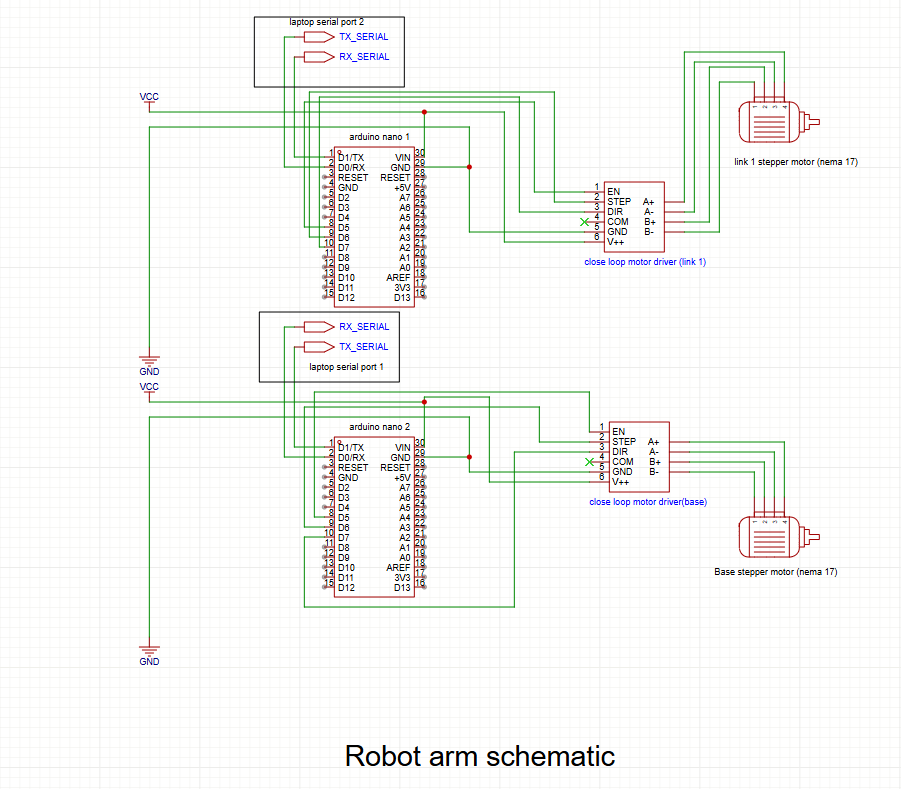
\includegraphics[width=0.95\linewidth]{pictures/arm_schamatic.png}
\caption{Electrical schematic of the robot arm control system, showing controller, drivers, and power distribution.}
\label{fig:arm_schematic}
\end{figure}

Two Arduino Nano microcontrollers implement a distributed control architecture. An on-board voltage regulator is used to regulate the supply to 
5\,V for the Arduino Nano. Each board receives joint-level position commands for its
assigned link via an independent serial interface and performs local trajectory generation, thereby decoupling the control loops for the base 
and shoulder. For the base joint, the software accounts for an effective transmission ratio of 30:1 when converting commanded angles to motor 
steps and velocity profiles.

Both actuators are driven by stepper motor drivers with microstepping to enhance positioning accuracy and disturbance rejection. The controllers 
interface with the microcontrollers using standard ENABLE, STEP, and DIRECTION control signals (as wired in Fig.~\ref{fig:arm_schematic}). The 
drivers commutate the motor phases by switching the A$+$, A$-$, B$+$, and B$-$ outputs; the polarity is governed by the DIRECTION input while 
incremental motion is effected by STEP pulses. Microstepping is employed to achieve smoother motion and increased effective resolution.


\section{Bill of Materials}

The bill of materials enumerates key mechanical and electrical components that satisfy the derived specifications while maintaining
 availability from multiple vendors. Selection criteria include performance-to-cost ratio, durability, interoperability with standard 
 interfaces, and lead time. Table~\ref{tab:components_bom} summarizes representative components used in the prototype.

\begin{table}[H]
\centering
\caption{Bill of materials for the manipulator prototype.}
\label{tab:components_bom}
\begin{tabular}{|p{0.28\linewidth}|c|p{0.30\linewidth}|p{0.30\linewidth}|}
\hline
Item & Qty & Specification & Function \\
\hline
T-slot aluminum extrusion & 2 & 4040 profile & Primary structural members \\
Harmonic drive & 1 & 30 to 1 gear reduction & Torque amplification \\
Stepper motor & 2 & NEMA 17, 1.8 deg/step & Joint actuation \\
Stepper driver & 2 & ENABLE/STEP/DIR inputs & Motor control \\
Microcontroller & 2 & Arduino Nano & Control and communication \\
Power supply & 1 & 12V, 5A & DC power source \\
Shielded cable & - & Twisted-pair & Wiring harness \\
3D printing filament (PLA) & 1 & 1 kg spool, 1.75 mm & Rapid prototyping of non-load parts \\
3D printing filament (PLA) & 1 & 1 kg spool, 1.75 mm & Durable housings and brackets \\
\hline
\end{tabular}
\end{table}


\section{Fabrication and Assembly}
Manufacturing methods include CNC machining for aluminum components (precision and durability), 3D printing for PLA plastic housings and brackets, manual assembly for component integration and cable routing, and calibration procedures for joint alignment and sensor setup. Dimensional tolerances are specified for bearing seats, pulley alignment, and shaft interfaces to ensure minimal backlash and consistent transmission efficiency. Quality control inspections are performed after each major operation, including visual inspection, dimensional verification with calipers/gauges, and rotational smoothness checks of assembled joints. All project CAD files referenced in this chapter are provided in Appendix~A for completeness and reproducibility.

\begin{figure}[H]
\centering
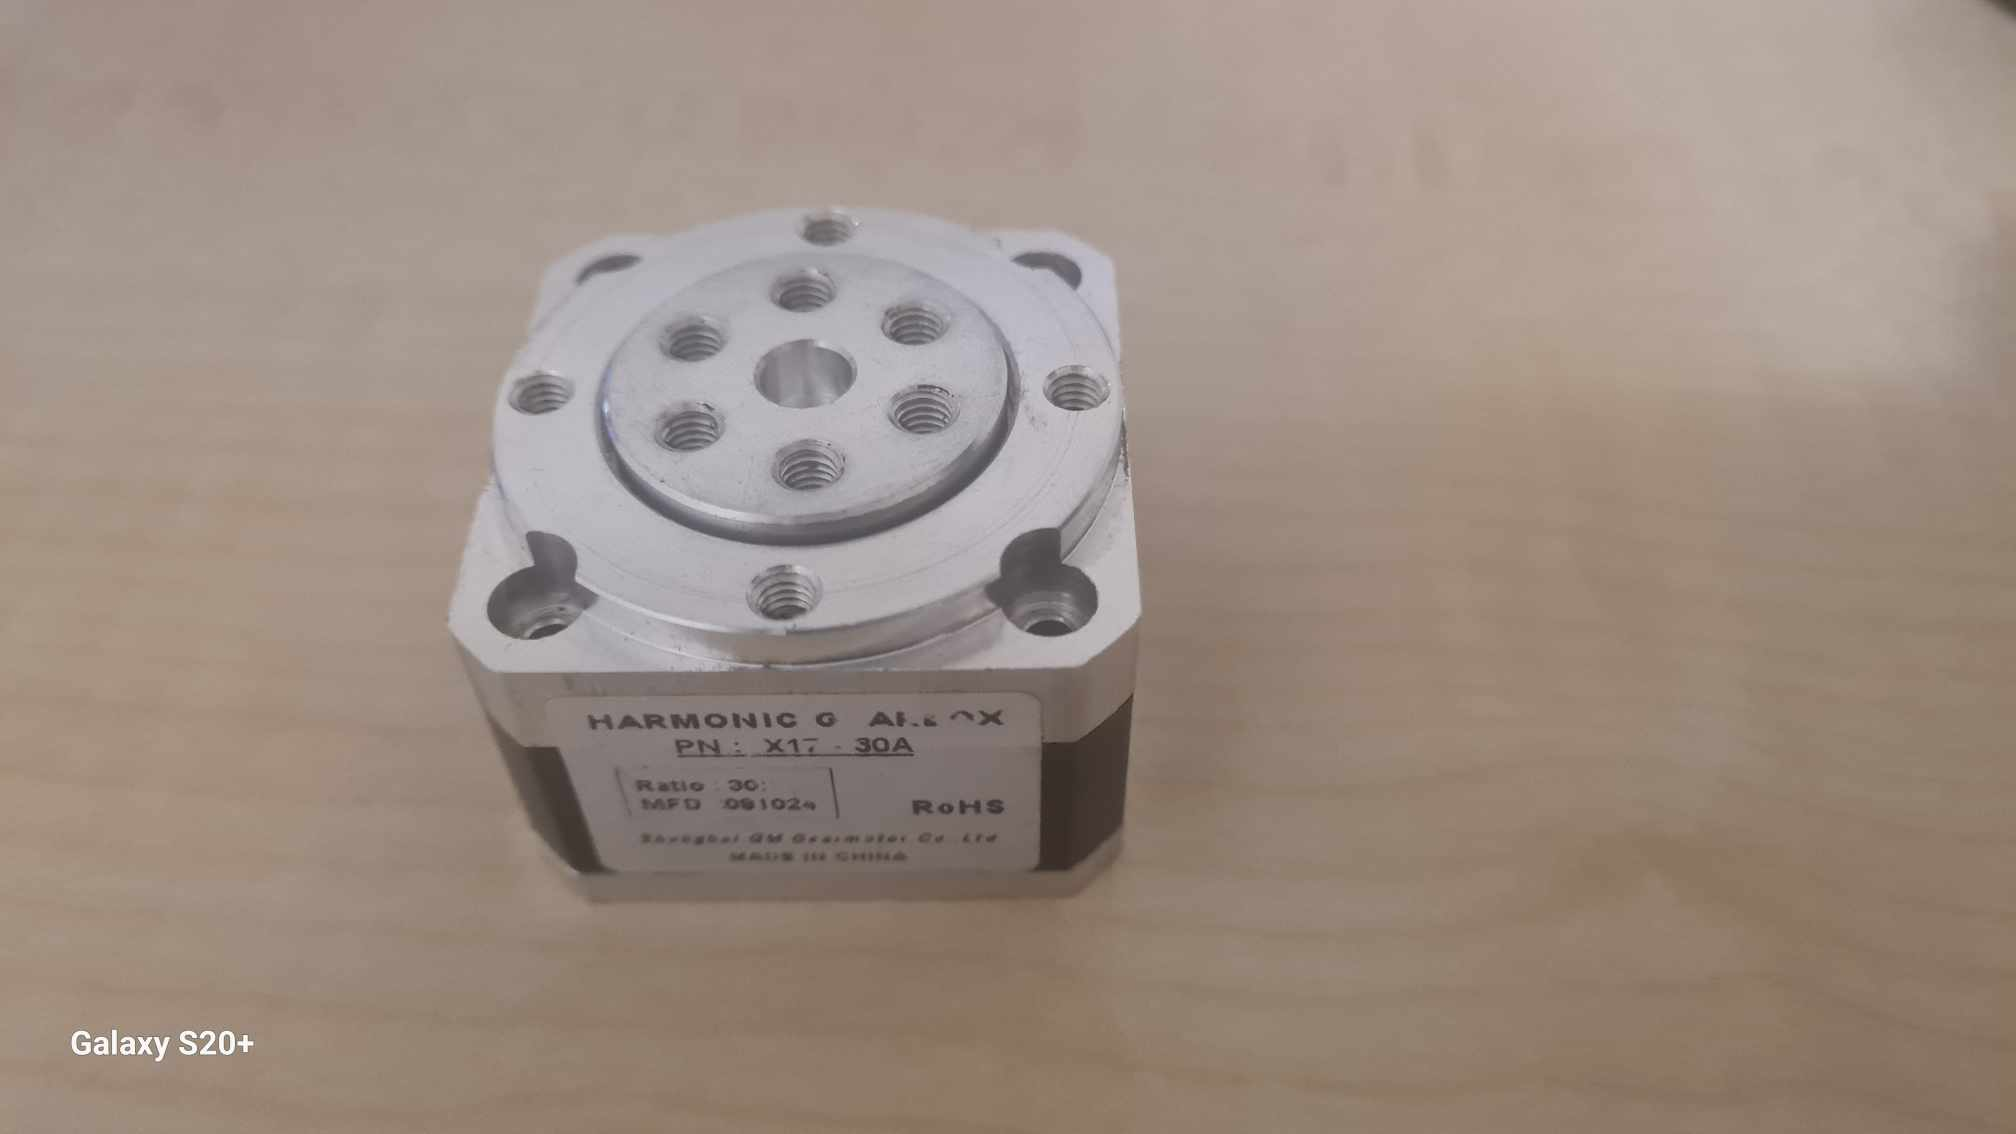
\includegraphics[width=0.48\linewidth]{pictures/gearreducer.jpg}\hfill
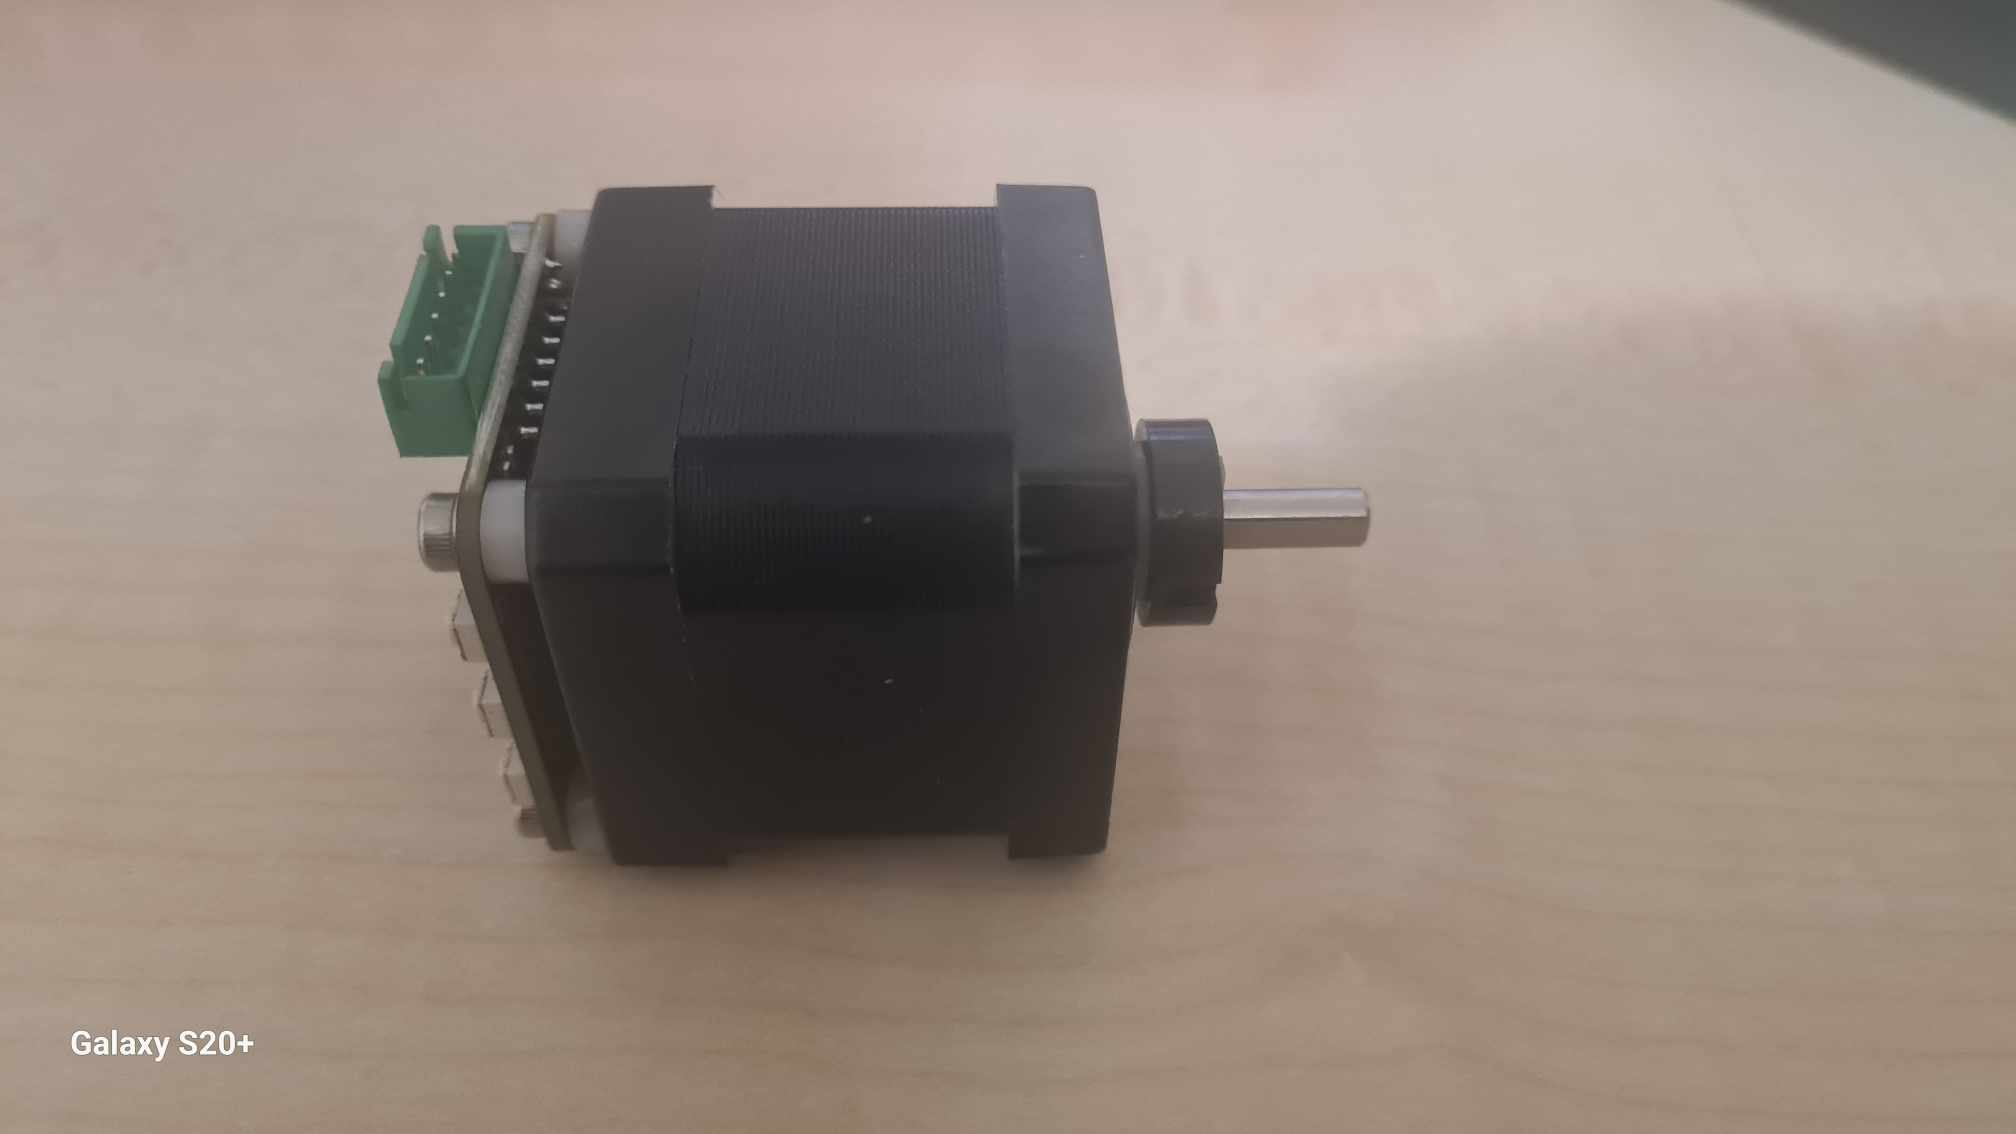
\includegraphics[width=0.48\linewidth]{pictures/nema17.jpg}
\caption{Prototype actuation hardware. Left: compact harmonic-drive gear reducer (30:1) used on the base joint to increase output torque and stiffness while maintaining low backlash. Right: NEMA 17 stepper motor (1.8 deg/step) employed for joint actuation, interfaced via ENABLE/STEP/DIR signals to the driver.}
\label{fig:actuator_photos}
\end{figure}

\begin{figure}[H]
\centering
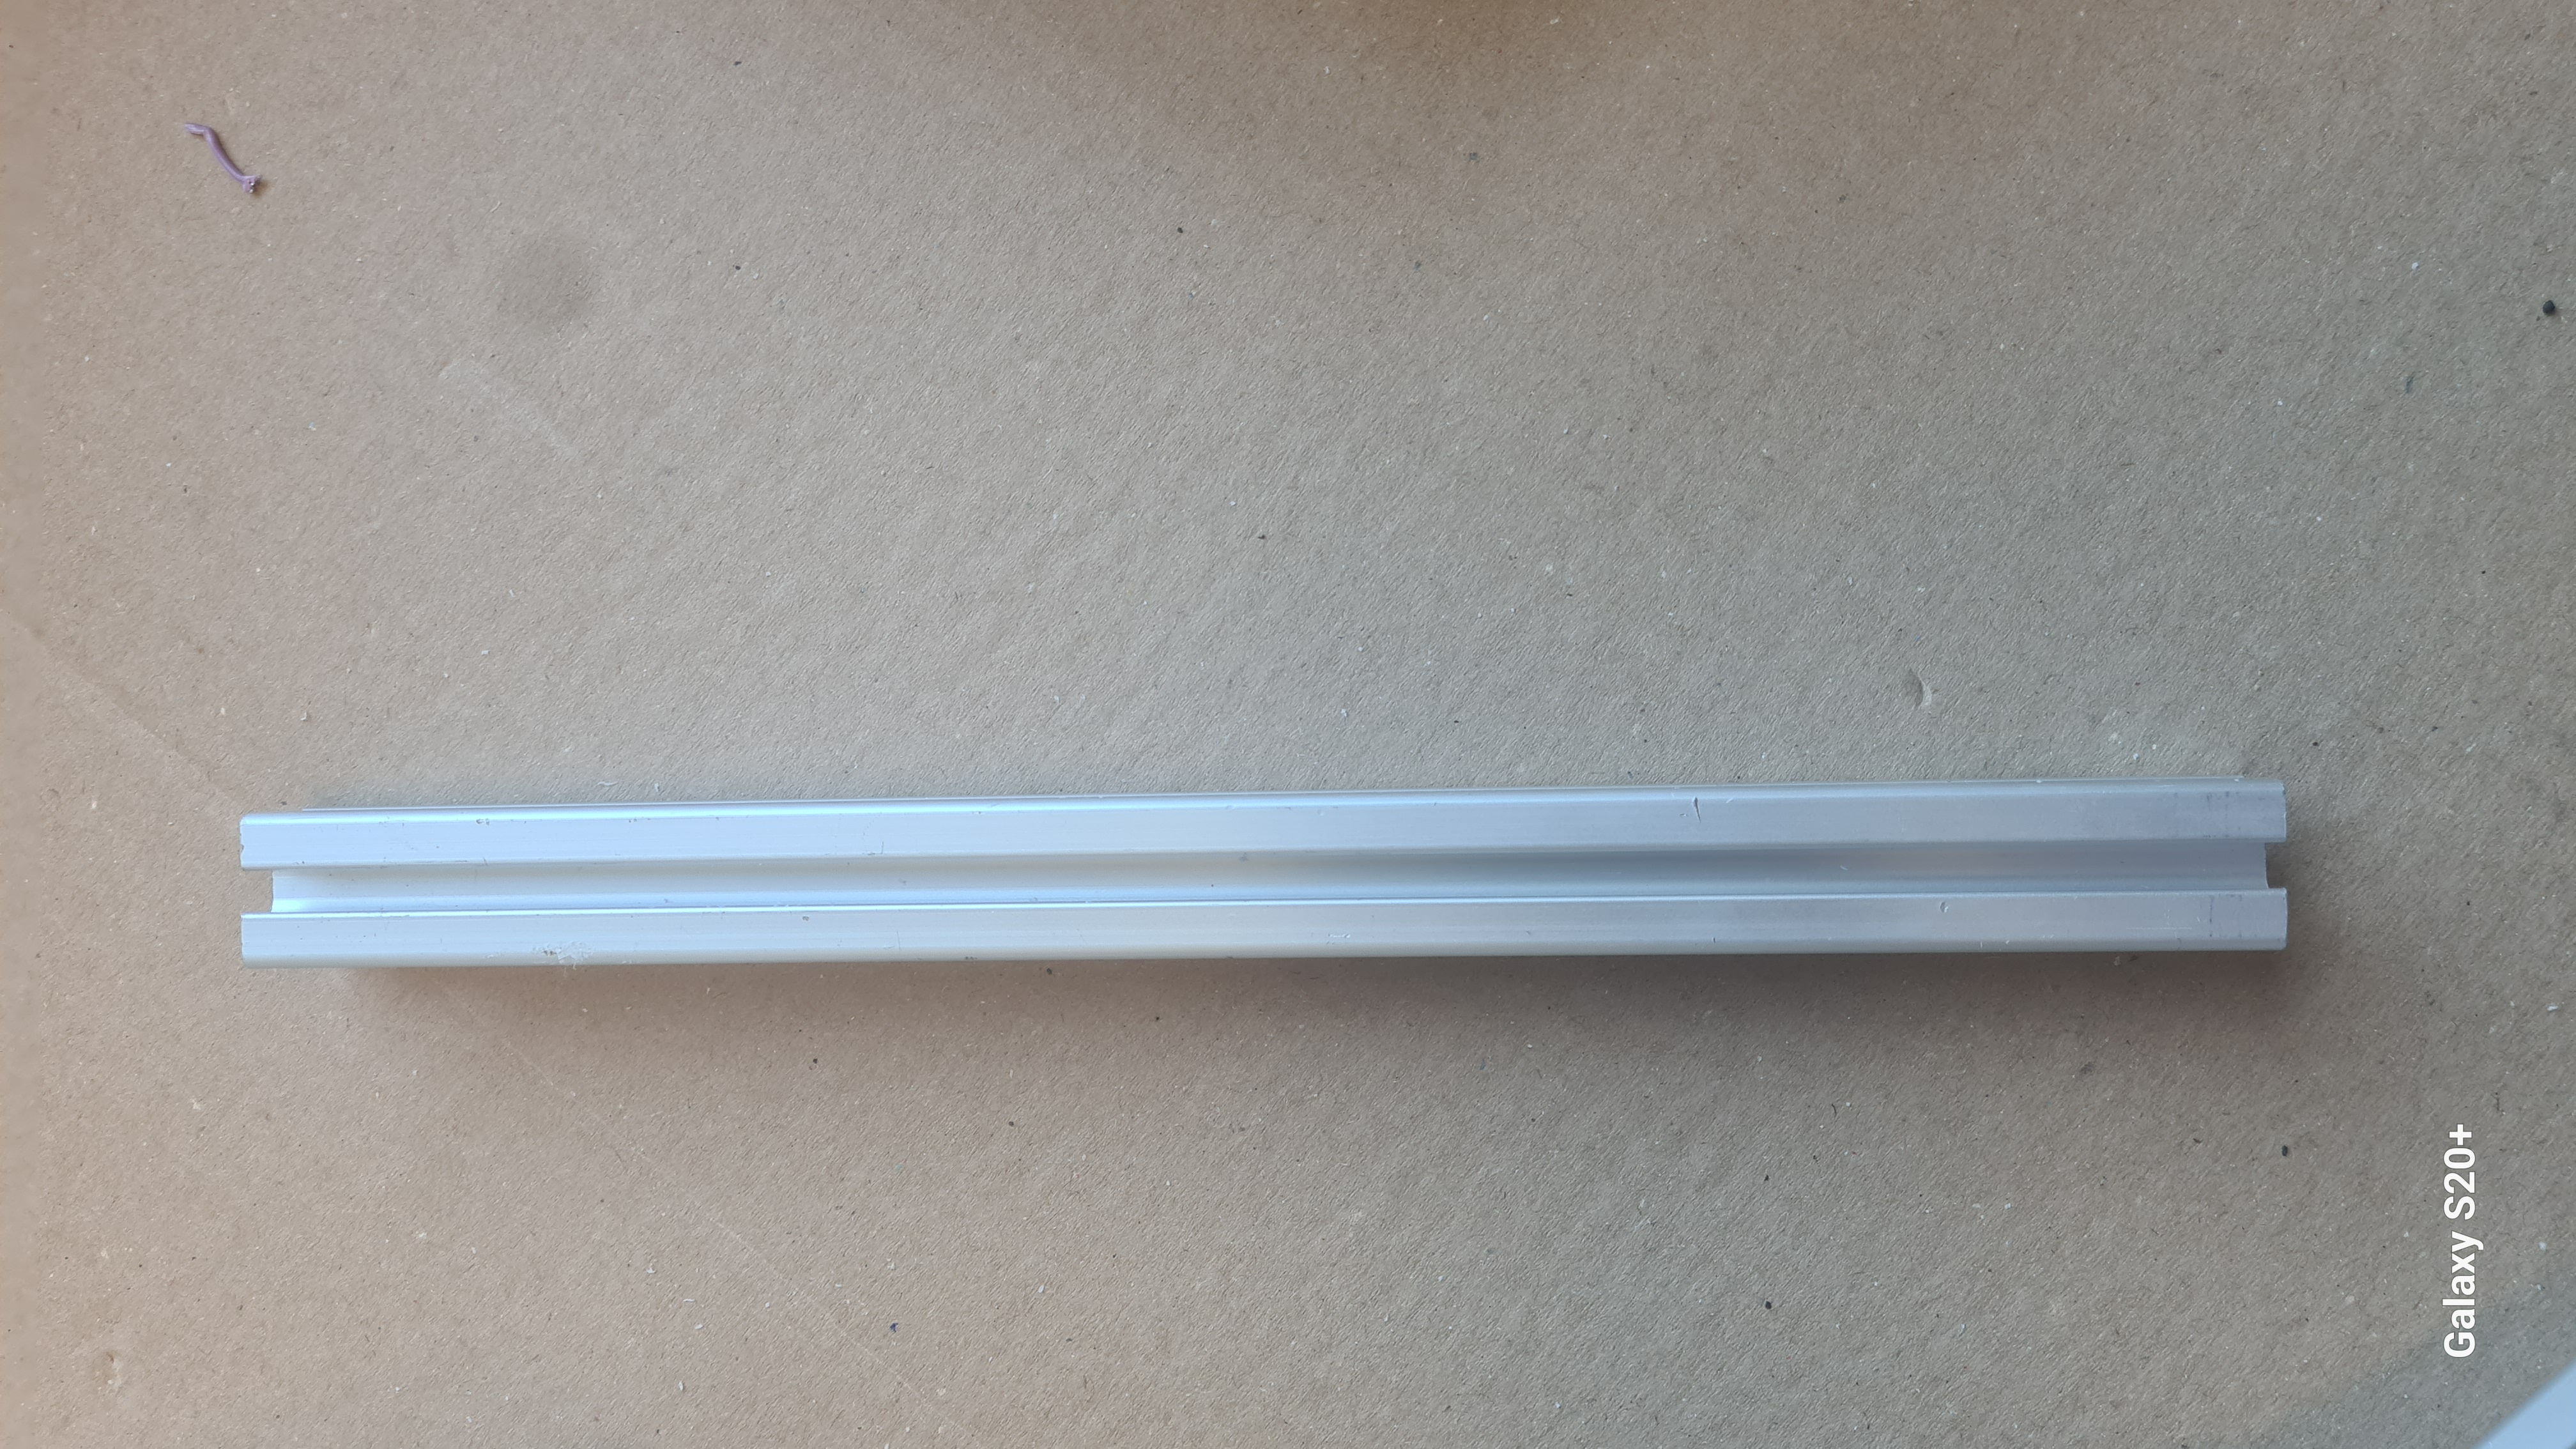
\includegraphics[width=0.48\linewidth]{\detokenize{pictures/ROD LINK.jpg}}\hfill
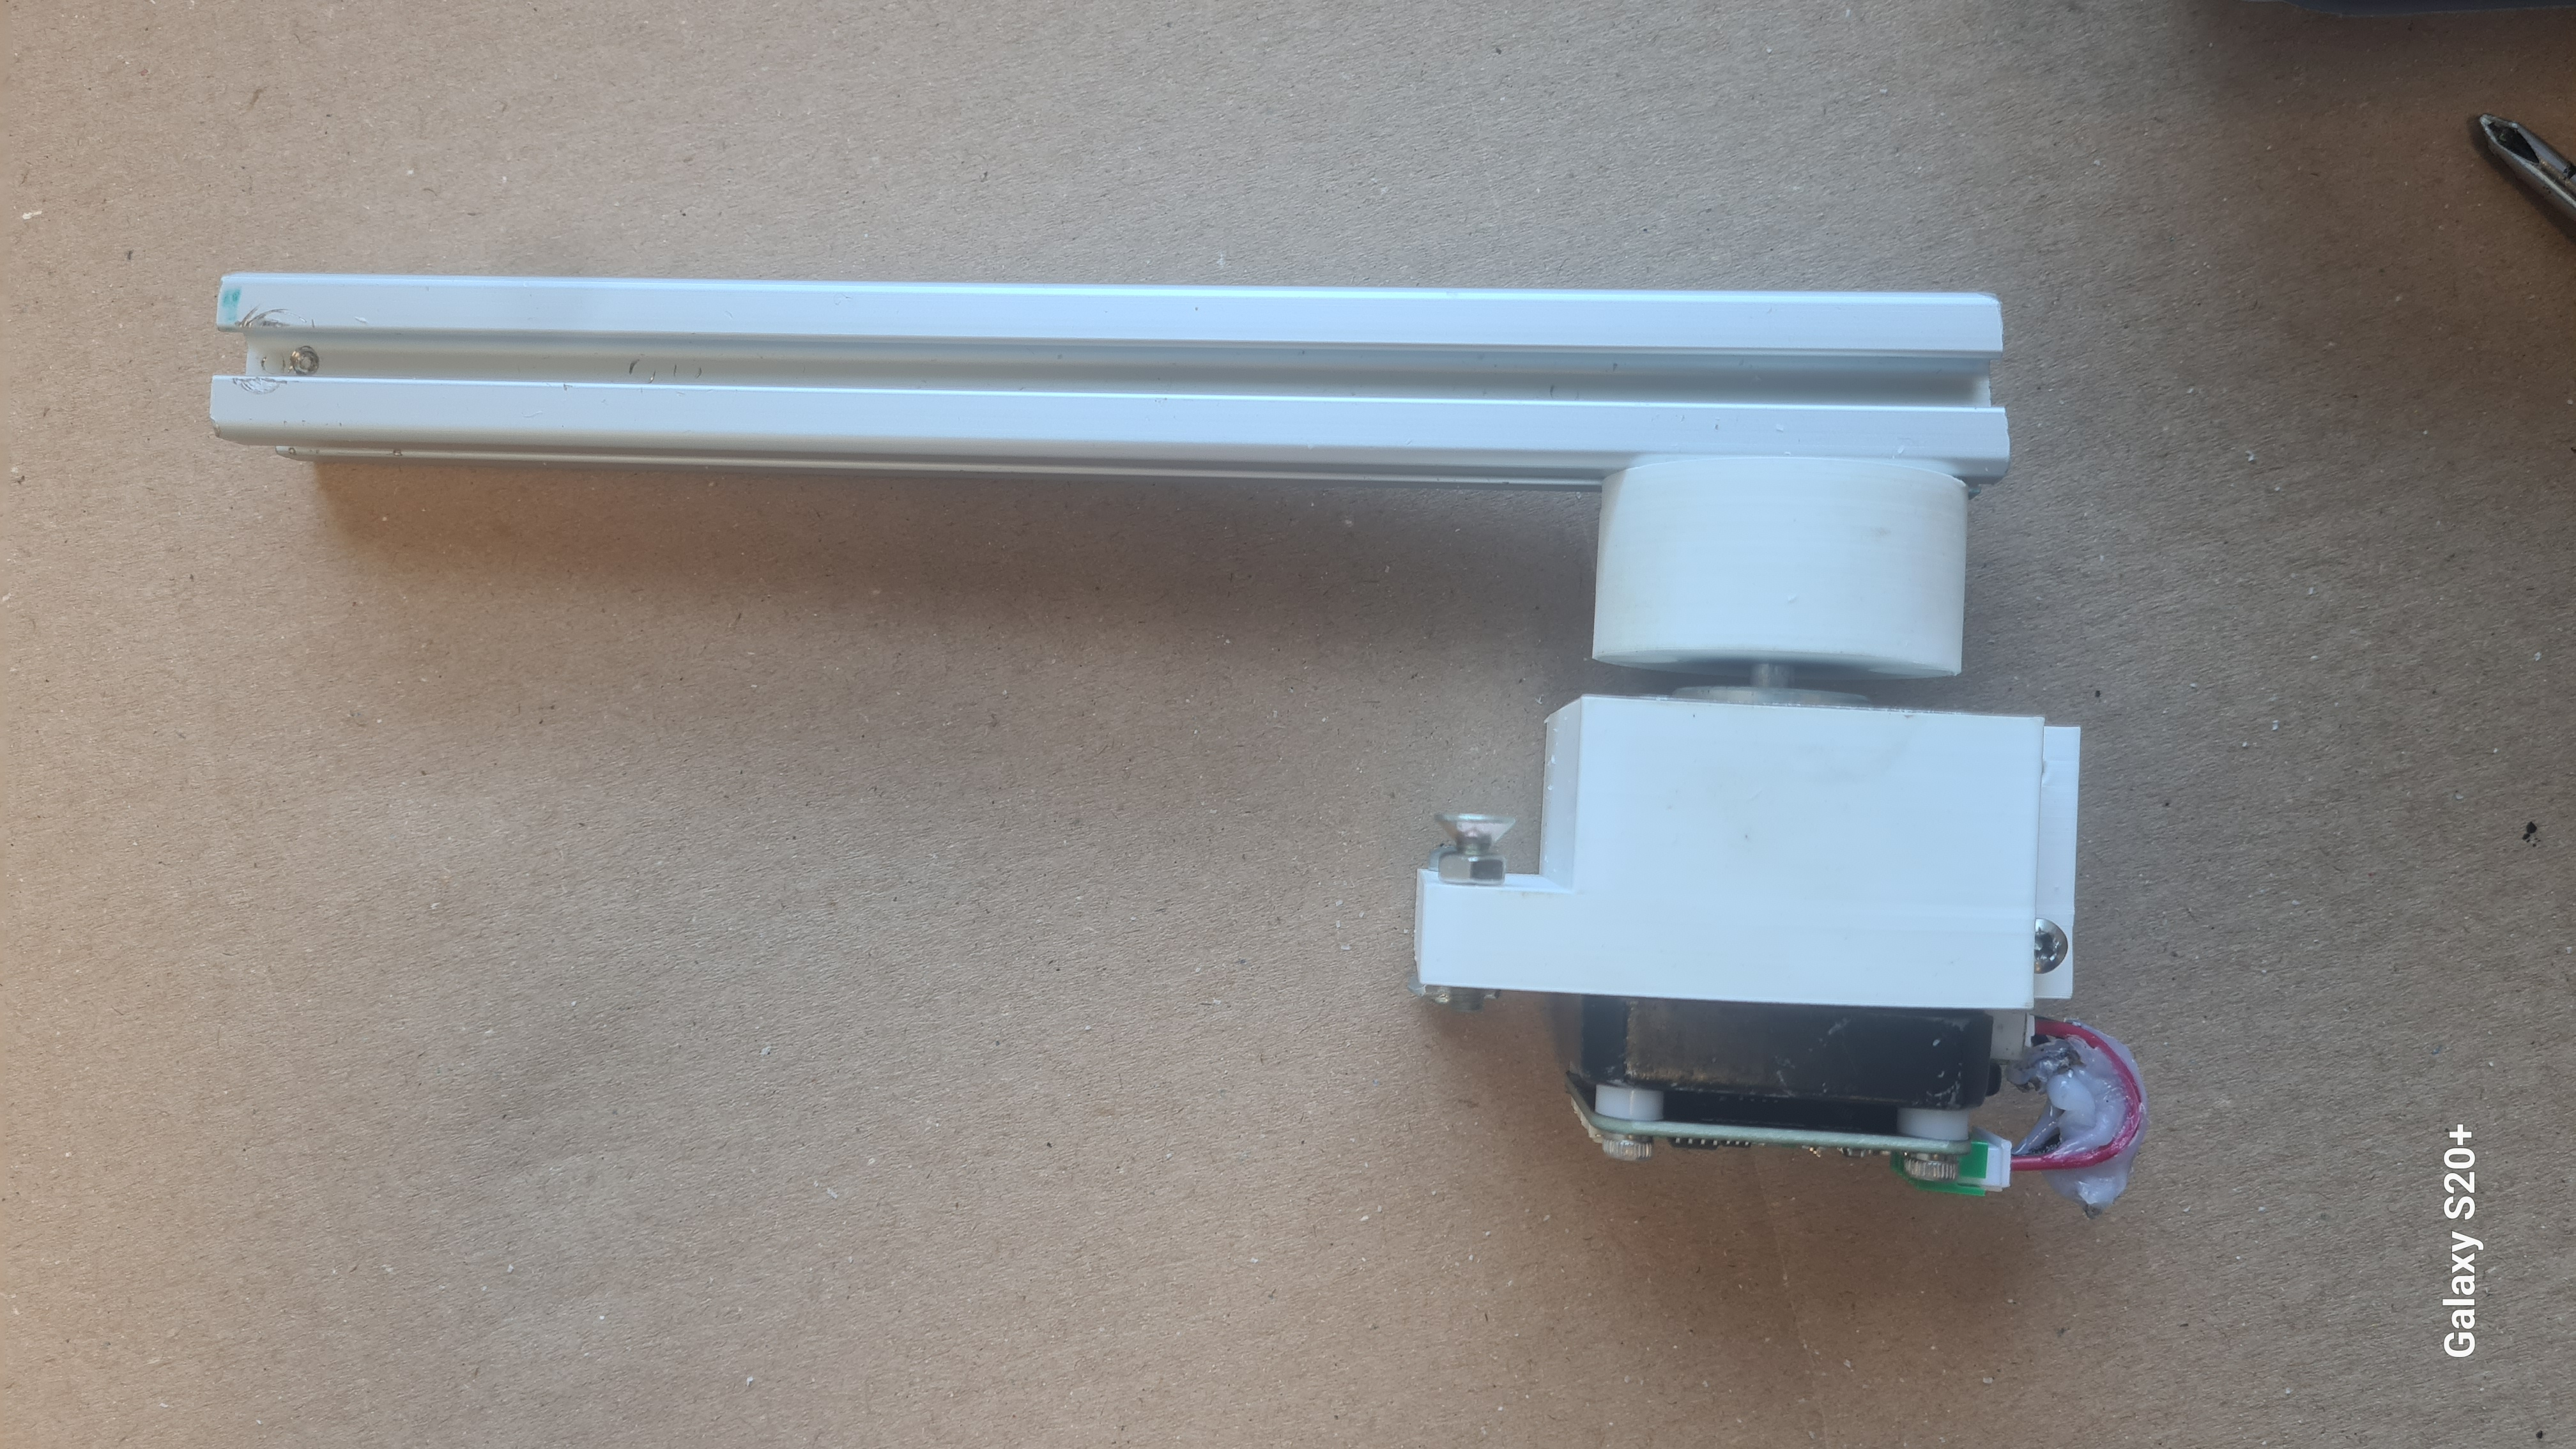
\includegraphics[width=0.48\linewidth]{\detokenize{pictures/shoulder assemble.jpg}}
\caption{Mechanical subassemblies. Left: machined aluminum rod link with T-slot profile used for lightweight, modular link construction. Right: shoulder assembly showing the link interface, printed mount, and fastener pattern enabling quick reconfiguration.}
\label{fig:link_and_shoulder}
\end{figure}

\begin{figure}[H]
\centering
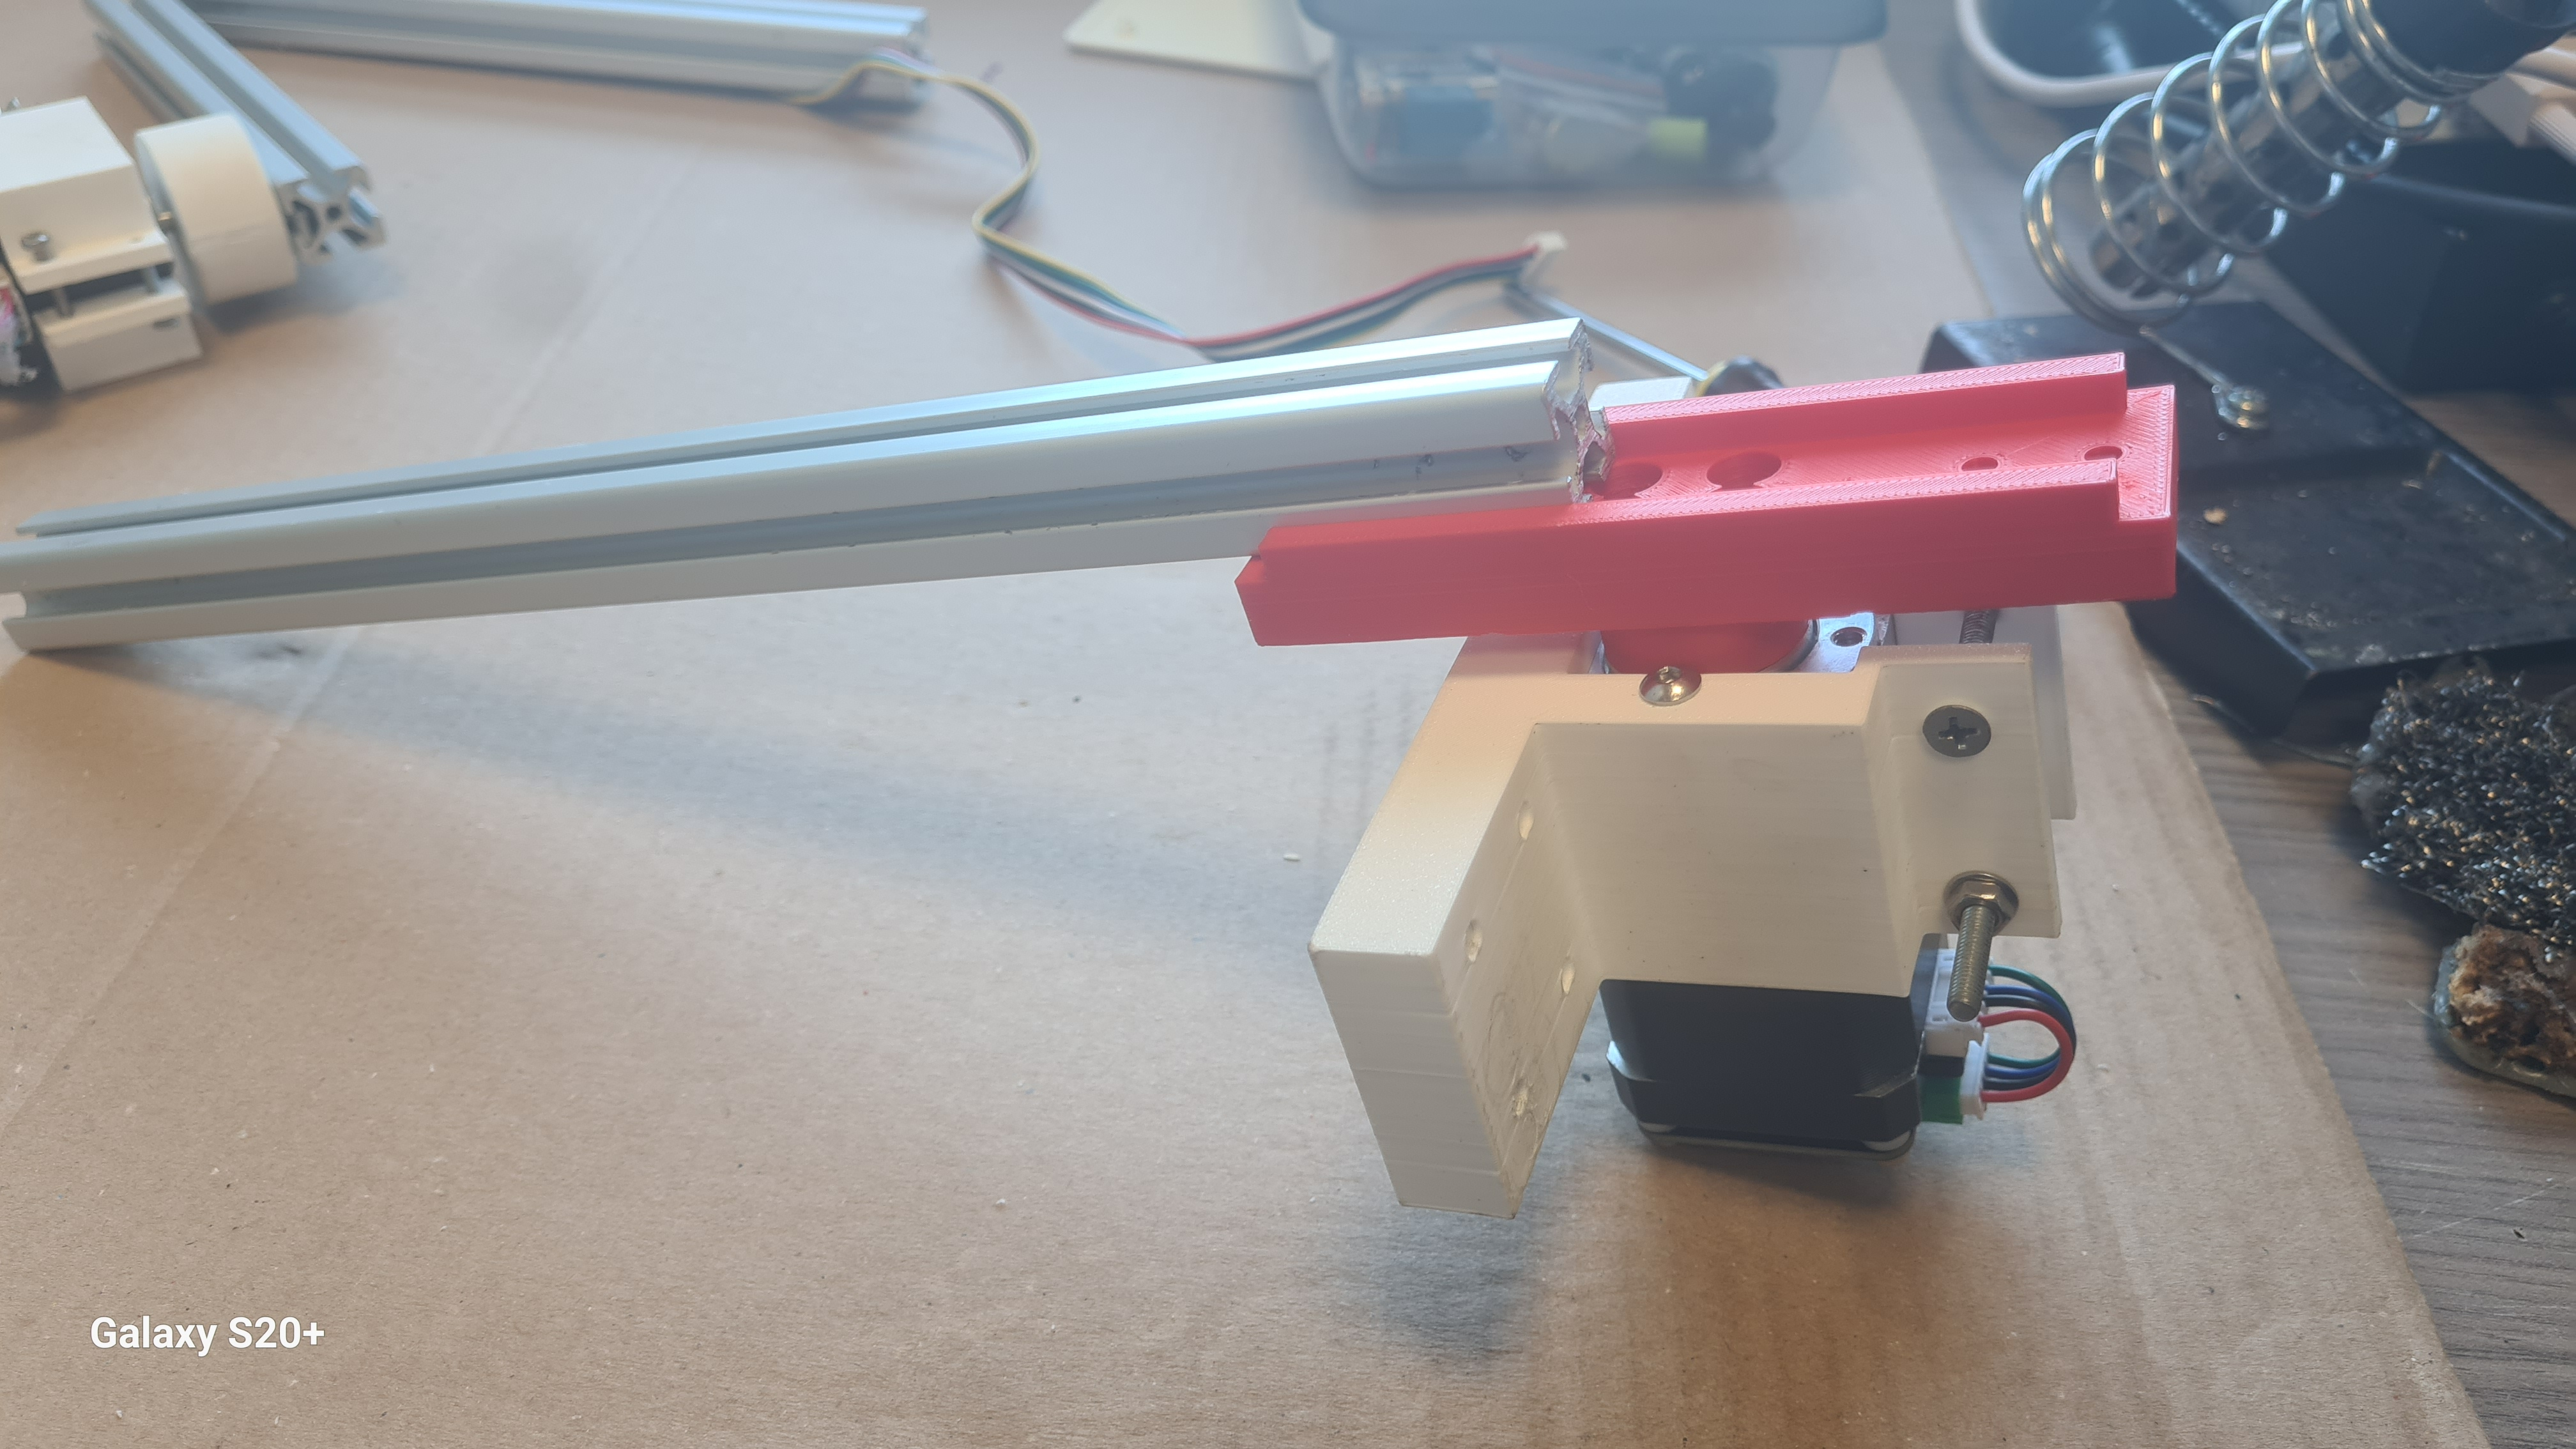
\includegraphics[width=0.48\linewidth]{\detokenize{pictures/BASE JOINT ASSEMBLE.jpg}}\hfill
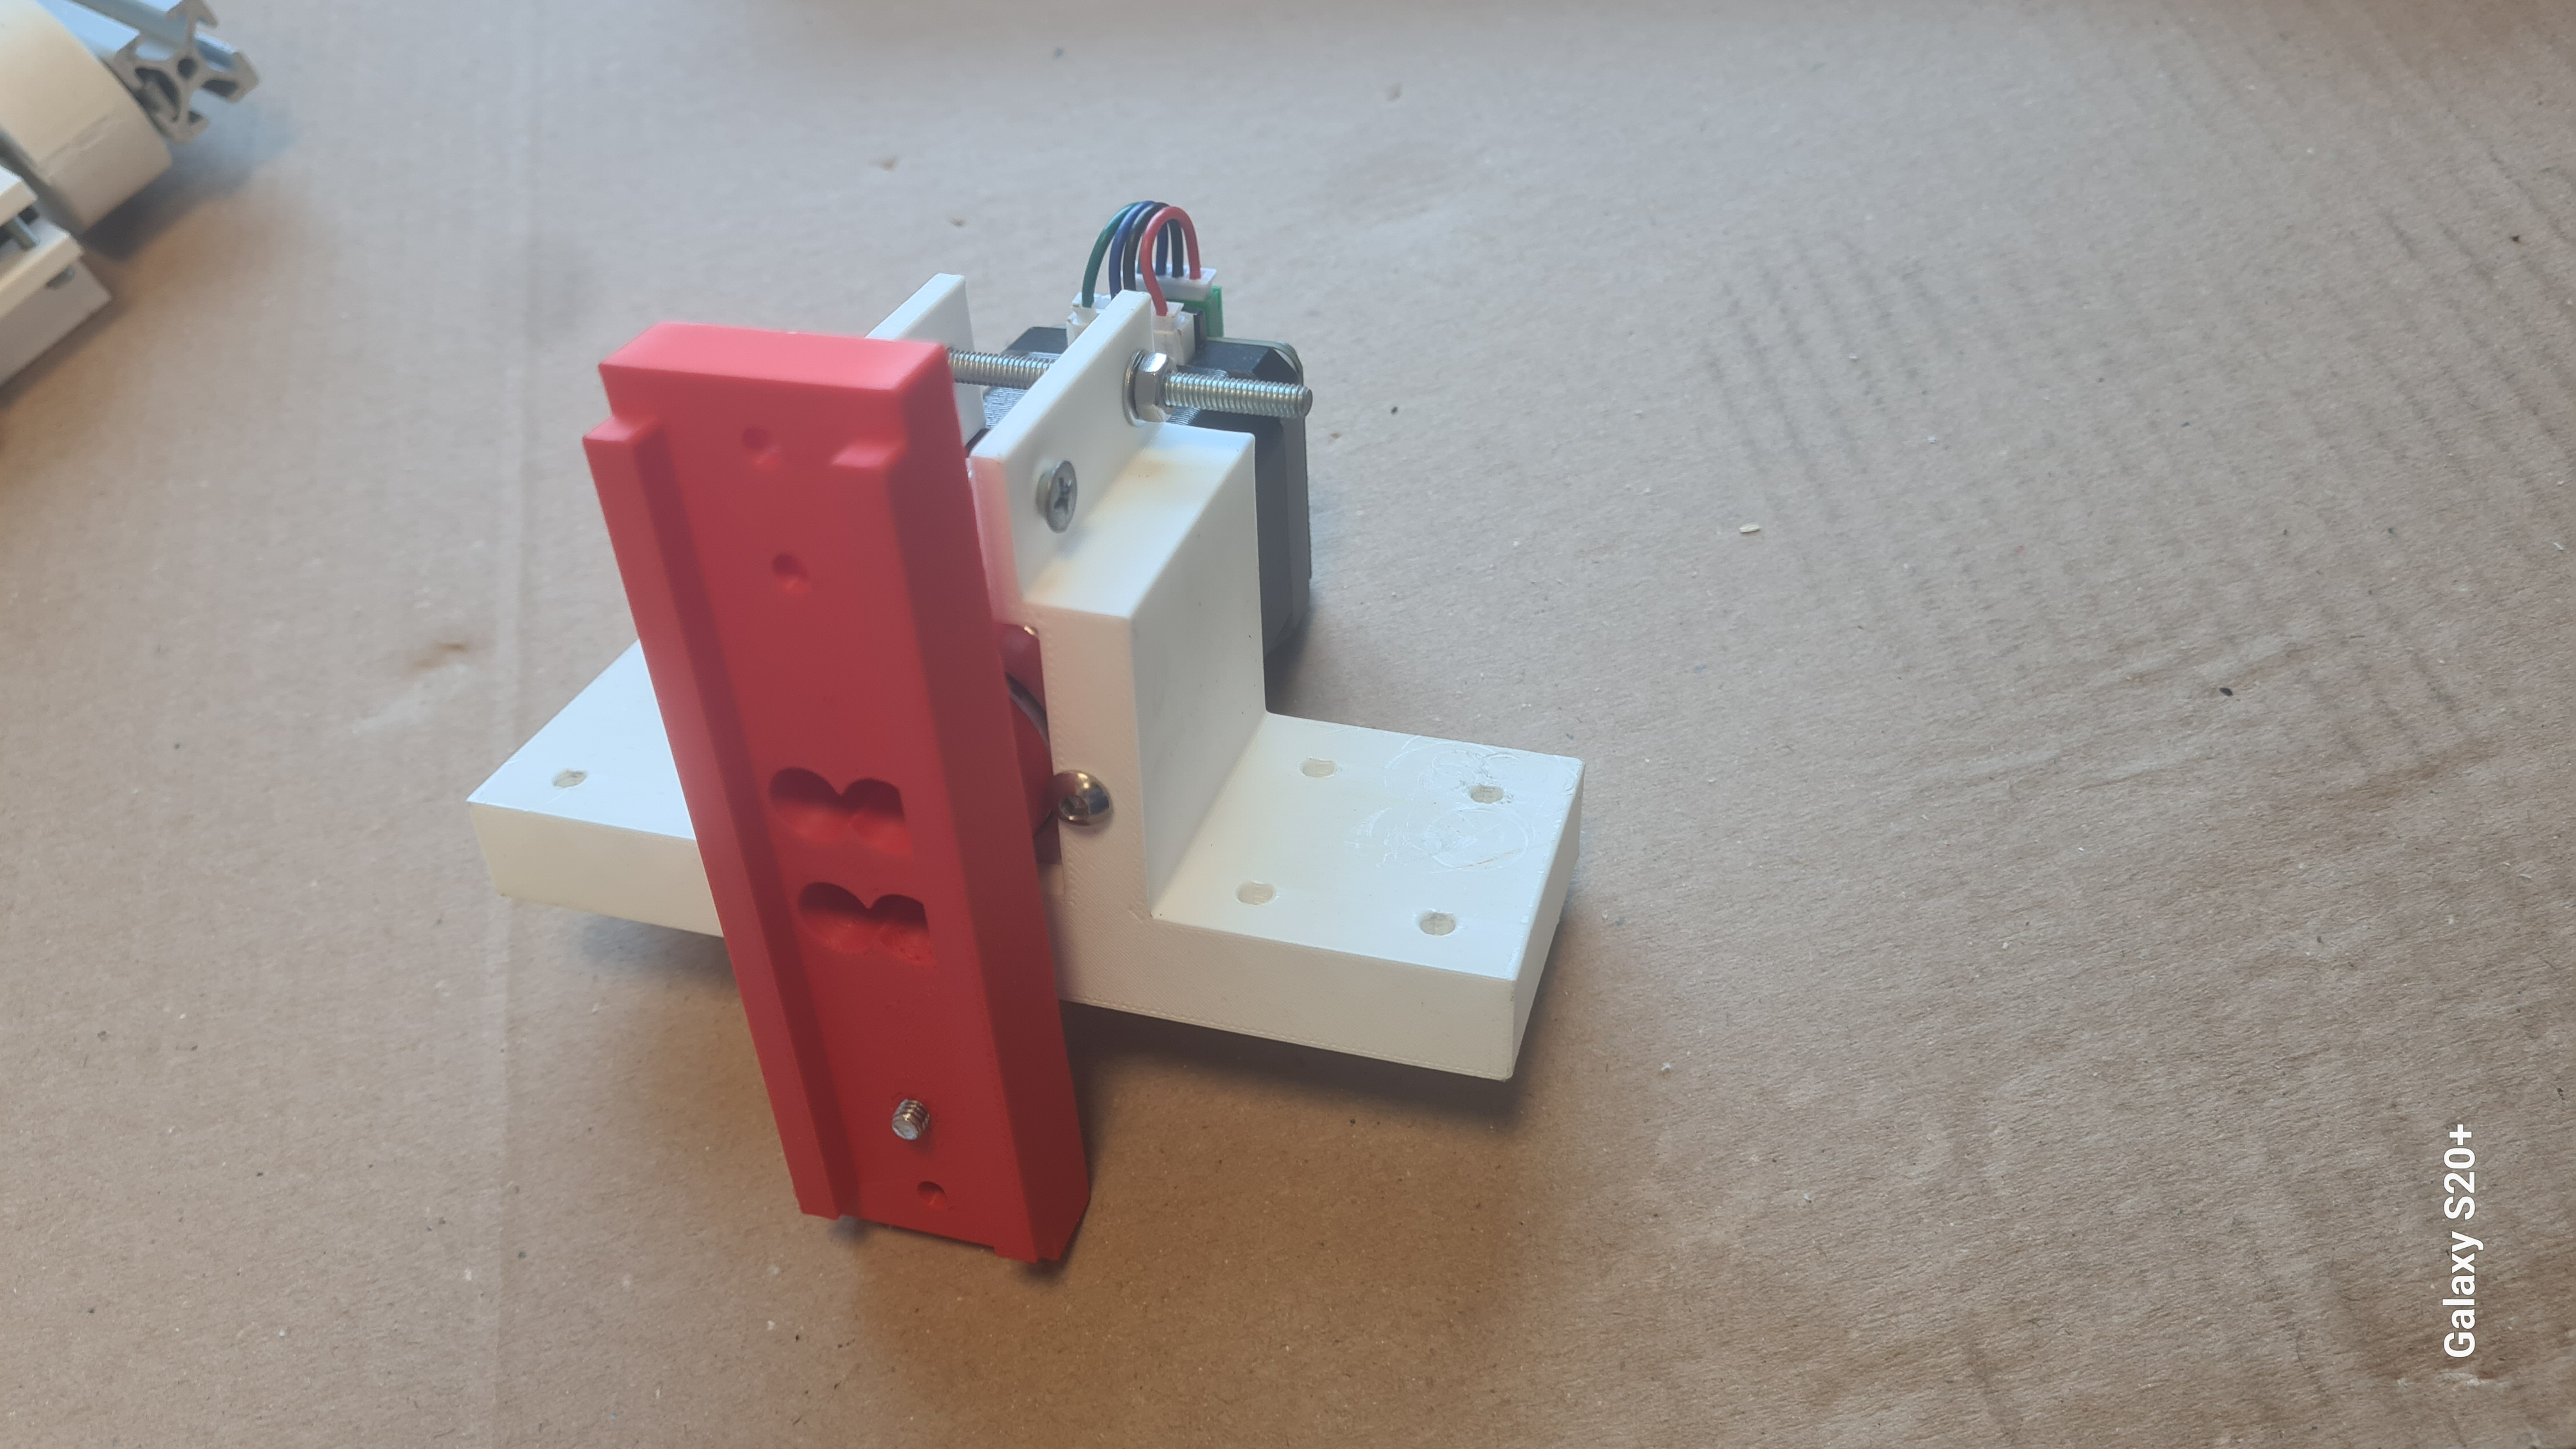
\includegraphics[width=0.48\linewidth]{\detokenize{pictures/BASE JOINT HOLDER.jpg}}
\caption{Base joint details. Left: assembled base joint integrating the gear reducer, stepper motor, and printed housing. Right: base-joint holder bracket that constrains the reducer and provides the structural interface to the frame.}
\label{fig:base_joint_details}
\end{figure}

\begin{figure}[H]
\centering
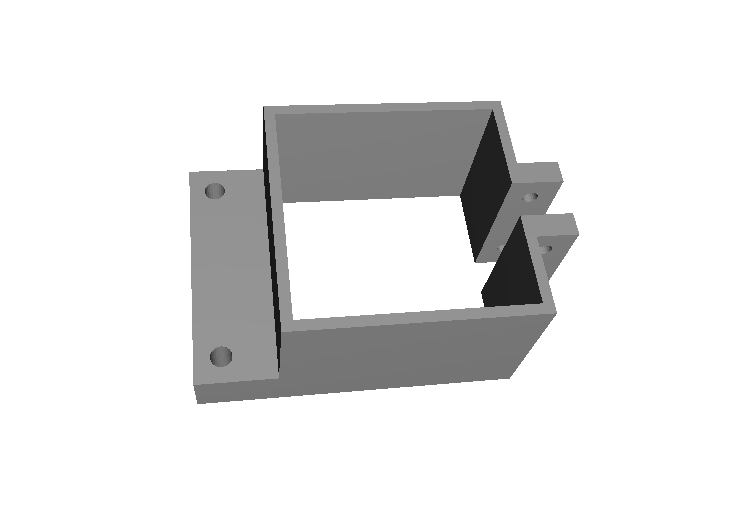
\includegraphics[width=0.48\linewidth]{\detokenize{pictures/stepper holder.png}}\hfill
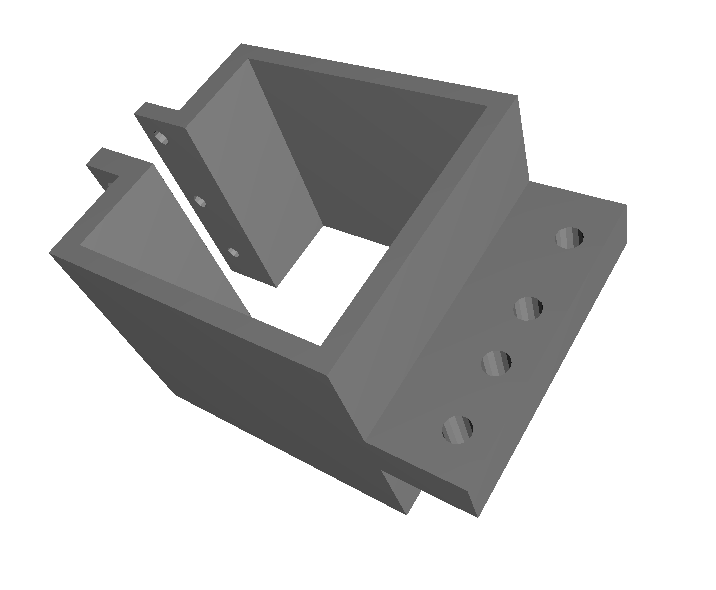
\includegraphics[width=0.48\linewidth]{\detokenize{pictures/stepperHolder.png}}
\caption{CAD snapshots of the stepper holder variants. Left: compact stepper holder with mounting flange for the NEMA 17 frame. Right: reinforced holder variant with additional fastener pattern for increased stiffness and alignment repeatability.}
\label{fig:stepper_holders}
\end{figure}

\begin{figure}[H]
\centering
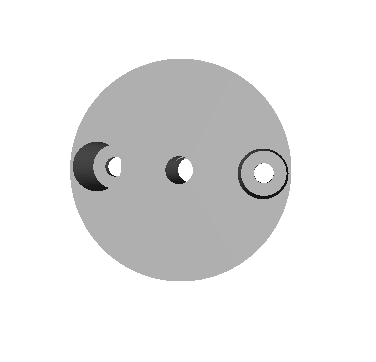
\includegraphics[width=0.48\linewidth]{\detokenize{pictures/shaft connector.png}}\hfill
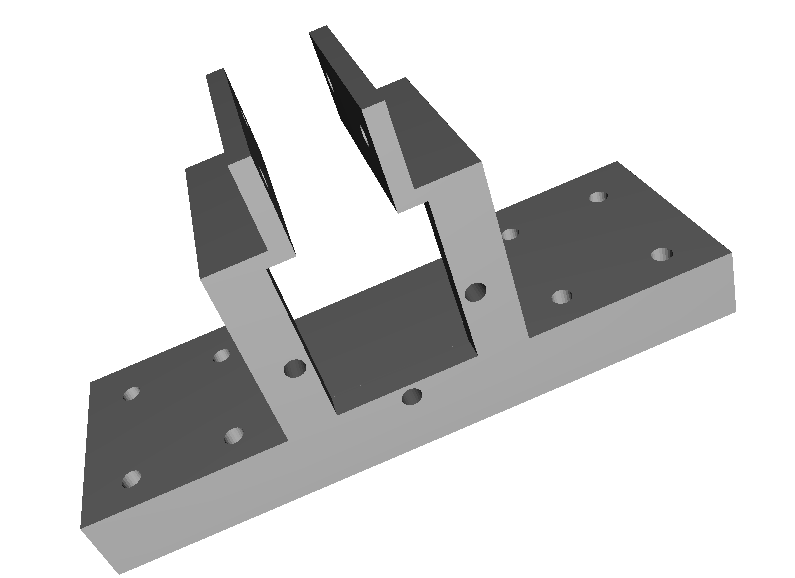
\includegraphics[width=0.48\linewidth]{\detokenize{pictures/base stepper holder.png}}
\caption{Additional CAD components. Left: shaft connector used to couple the stepper shaft to the reducer input while preserving concentricity. Right: base stepper holder showing the through-holes and counterbores that interface to the frame and allow cable clearance.}
\label{fig:connector_and_baseholder}
\end{figure}

\begin{figure}[H]
\centering
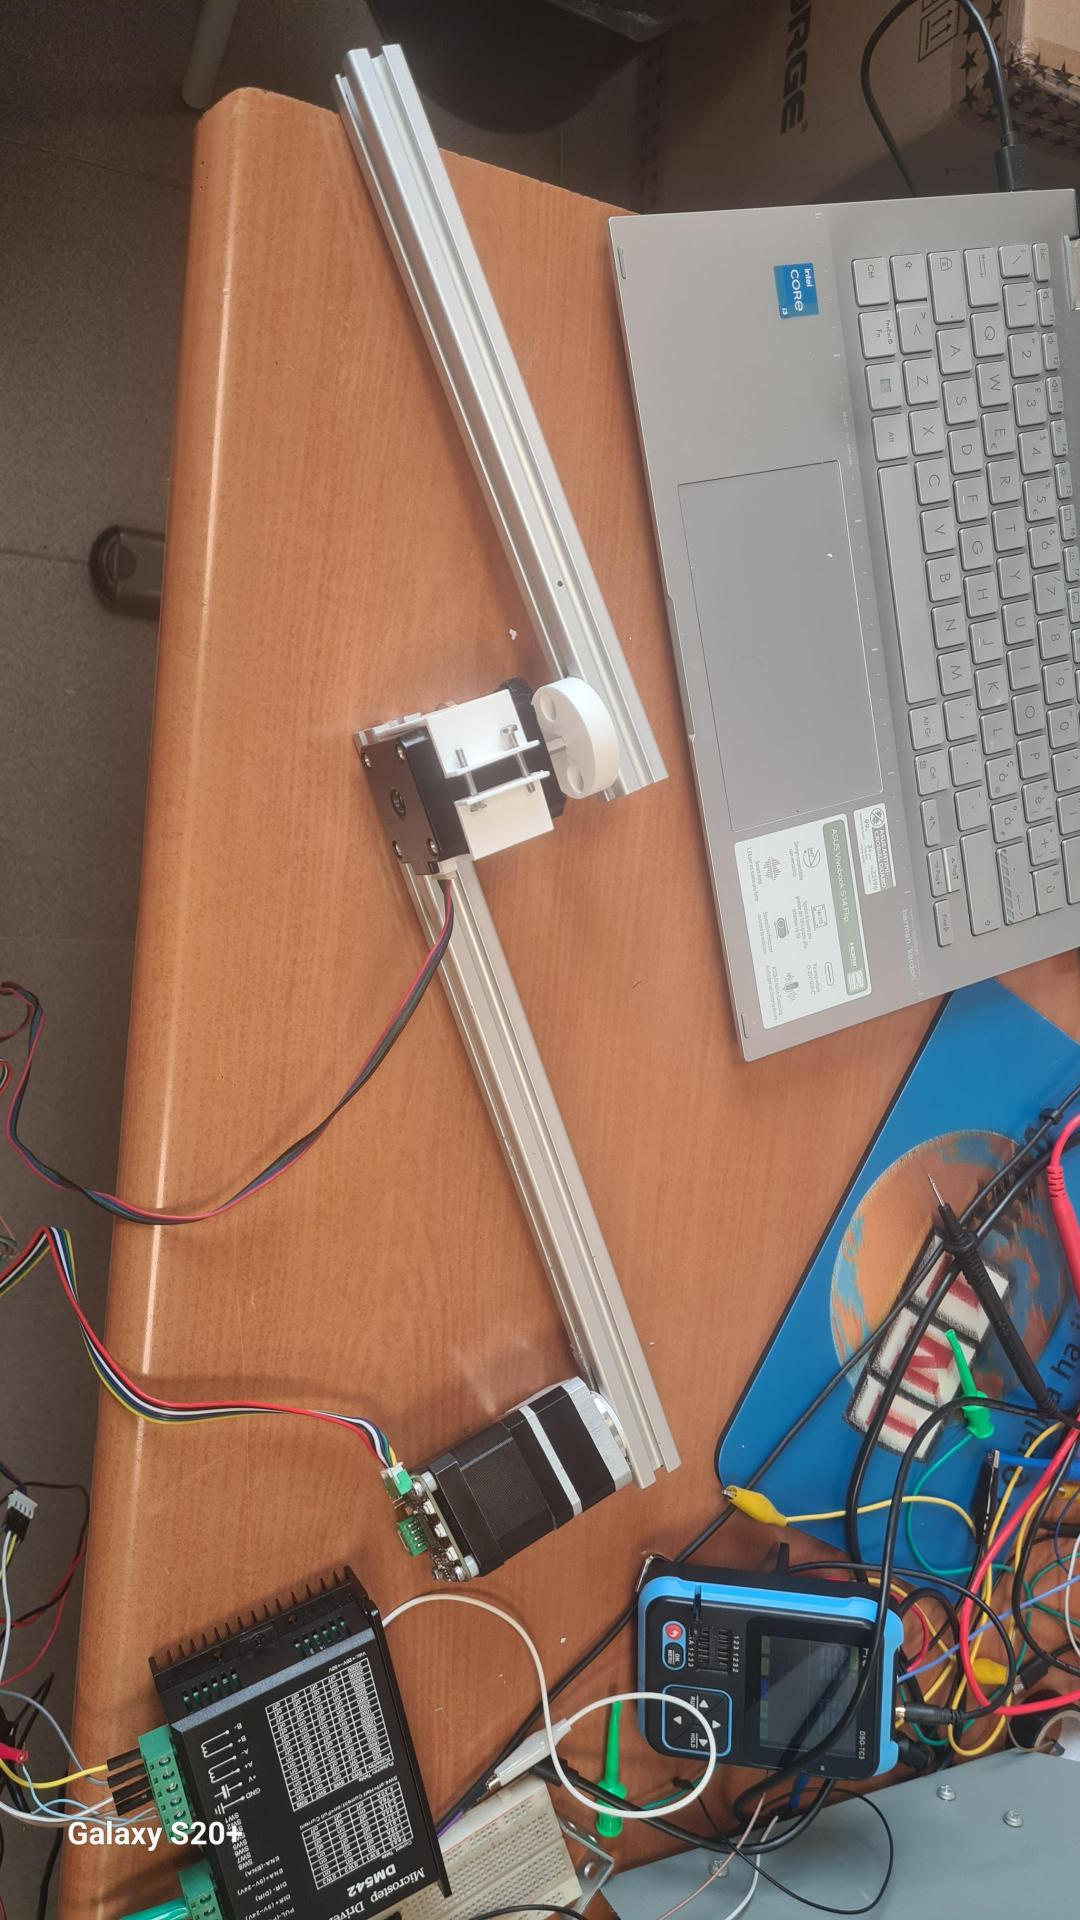
\includegraphics[width=0.7\linewidth]{\detokenize{pictures/semi assembled arm.jpeg}}
\caption{Bench test of the semi-assembled arm showing the base joint, shoulder link, stepper driver, and temporary wiring used for functional verification prior to full integration.}
\label{fig:semi_assembled_arm}
\end{figure}

The assembly sequence follows: (1) Base assembly with motor mounting and wiring, (2) Shoulder joint integration with gear reduction, (3) Forearm assembly with cable routing, (4) Wrist mechanism and end-effector mounting, (5) Electrical system integration and testing, (6) Final calibration and performance validation. Post-assembly calibration includes homing routine verification, limit-switch alignment, and zero-offset determination for each joint to establish a consistent reference frame for control and testing.

\section{Testing and Validation}

\subsection{Testing Protocol}
Comprehensive validation includes mechanical testing (static load testing for structural integrity under maximum payload, dynamic testing for motion smoothness and vibration analysis, repeatability testing for position accuracy over multiple cycles, endurance testing for long-term operation), electrical testing (power consumption analysis under various loads, signal integrity testing for communication reliability, safety system validation for emergency stop and limit switch functionality, control system testing for response time and accuracy), and integration testing (end-to-end functionality verification, software integration with control algorithms, performance benchmarking against design specifications, user acceptance testing for usability and reliability). Instrumentation may include encoders for joint position tracking, external motion capture or laser distance measurement for ground-truth accuracy, current sensing for driver characterization, and accelerometers for vibration assessment. Experimental sampling rates and trial counts are selected to ensure statistical significance and repeatability.

\subsection{Performance Analysis}
This subsection will present a comparative analysis of measured performance against the stated requirements, including accuracy, repeatability, payload capacity, and dynamic response. Results will be summarized with descriptive statistics and confidence intervals where appropriate, and discrepancies will be interpreted in light of modeling assumptions and manufacturing tolerances. The analysis will also identify predominant error sources (e.g., compliance, backlash, controller tuning) and propose targeted design or control refinements for subsequent iterations.


\chapter{GRIPPER DESIGN}
\graphicspath{{./}{pictures/}{inventor/}}
\section{Requirements of objective}
Picking asparagus with a robotic arm requires a carefully coordinated process that prioritises gentle handling and consistent performance while minimising damage to the plant. The gripper must interface reliably with slender, fragile spears, accommodating natural variability in diameter, length, and orientation. To enable this, the system first detects the presence of asparagus plants in the field and accurately estimates the position, pose, and size of individual spears.

Perception can be achieved using cameras, LiDAR, or a sensor fusion approach that balances accuracy, robustness, and cost. Visual or depth sensing provides the measurements necessary to localise each spear within the robot’s workspace and to categorise targets according to maturity and suitability for harvesting. These classifications inform grasp strategy—such as contact location, applied force, and approach vector—so that the gripper can secure the spear without bruising, bending, or uprooting adjacent growth. This sensing-to-action pipeline underpins the design requirements for the gripper, ensuring that mechanical, sensing, and control choices collectively support precise, repeatable, and low-damage harvesting.




\section{Finger design}
For a finger design to pick and chop the stem of asparagus, I have set up a design based on
two fingers which will hold the asparagus stem down by a mg995 servo motor adjunct with a
and a blade holder underneath the finger also driven by another servo mg995. The whole
design is worked on inventor 2025 as it could be seen below


\begin{figure}[H]
    \centering
    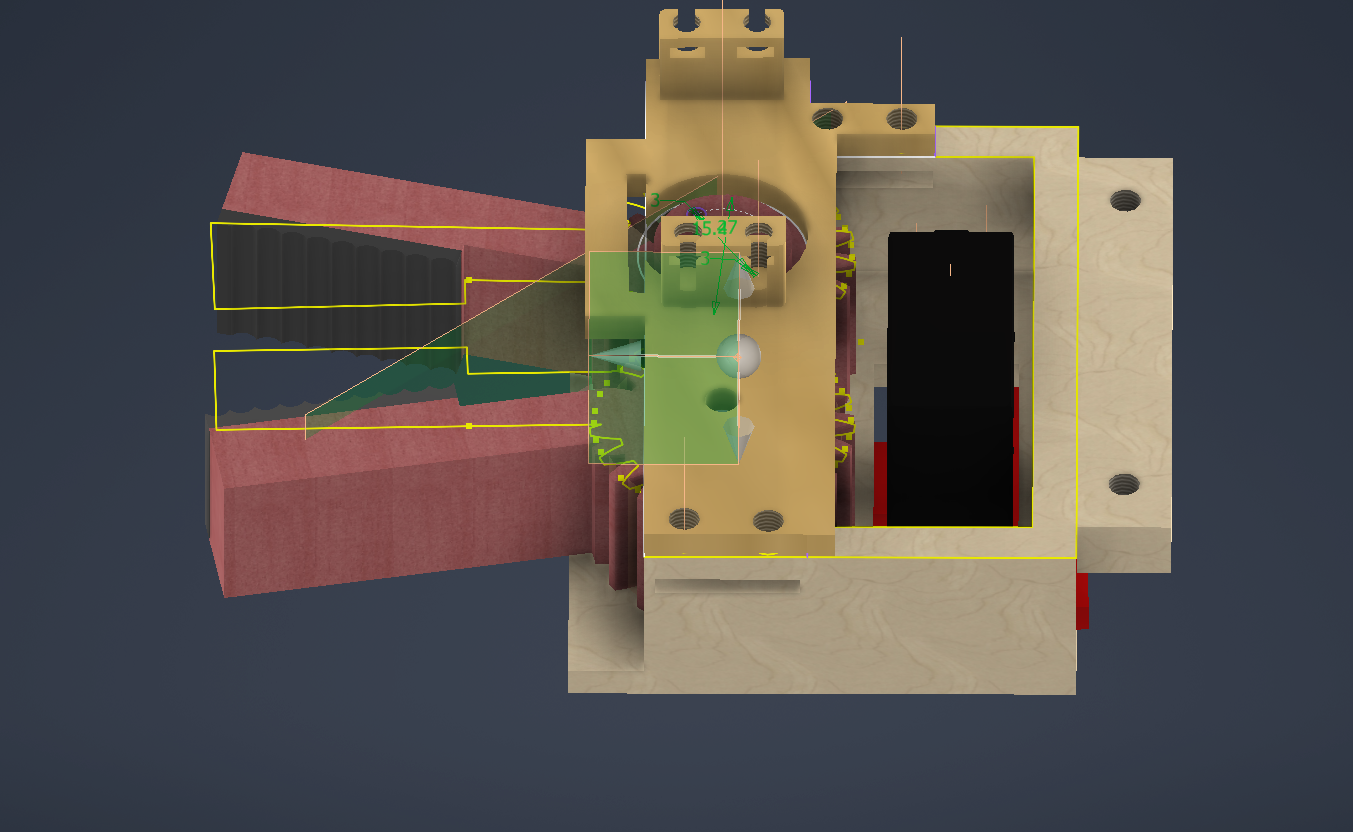
\includegraphics[width=0.9\textwidth]{finger_design_inventor.png}
    \caption{Finger design developed in Inventor 2025 showing kinematics and packaging.}
    \label{fig:finger_inventor}
    \end{figure}








The red component in Figure~\ref{fig:finger_inventor} denotes the finger module, which achieves a
form-closure grasp on the asparagus spear. The grasping strategy is intentionally conservative to
avoid bruising or buckling of the slender stem. To this end, the contact surfaces are equipped with
compliant, sponge-like pads that deform elastically, distributing pressure over a larger area and
attenuating transient load peaks during closure. The applied normal force is limited to a target
maximum of approximately 10\,N, which is adopted as a safe threshold for handling without damage
based on empirical observations from preliminary trials.

To verify that these constraints are satisfied across expected geometric and material variability, the
finger will be evaluated through a combination of quasi-static and dynamic analyses. The study will
include contact modelling of the pad–spear interface, estimation of required actuation torque under
frictional form closure, and time-domain simulations to quantify impact forces during grasp onset and
blade engagement. These results will inform controller tuning and pad material selection, ensuring the
design achieves reliable retention while preserving the integrity of the crop.



To quantify actuator demands, a time-domain dynamic analysis was performed to estimate the
resultant torque at the finger joint under a conservative handling load. Assuming a maximum
allowable contact force of approximately 10\,N at the fingertip, the corresponding joint torque
was computed over the grasping trajectory. The simulation was executed in Autodesk Inventor
2025 using 100 time steps to capture transient effects and peak values in Decinewton (dN). The resulting torque
profile is shown in Figure~\ref{fig:finger_torque}.
\begin{figure}[H]
    \centering
    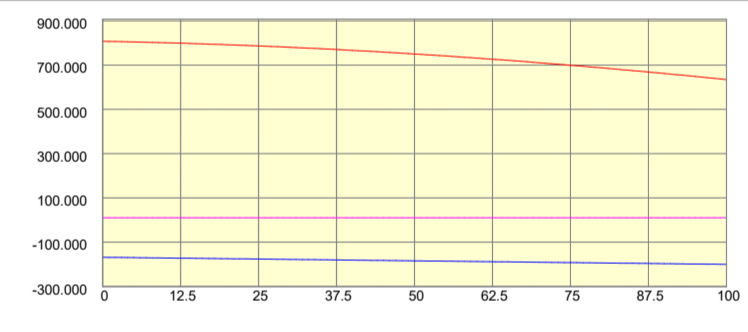
\includegraphics[width=0.75\textwidth]{fingerforceDynamics.png}
    \caption{Computed finger joint torque over the grasping trajectory (100-step dynamic analysis).}
    \label{fig:finger_torque}
    \end{figure}

    


\section{Electrical schematic and operation}


\begin{figure}[H]
    \centering
    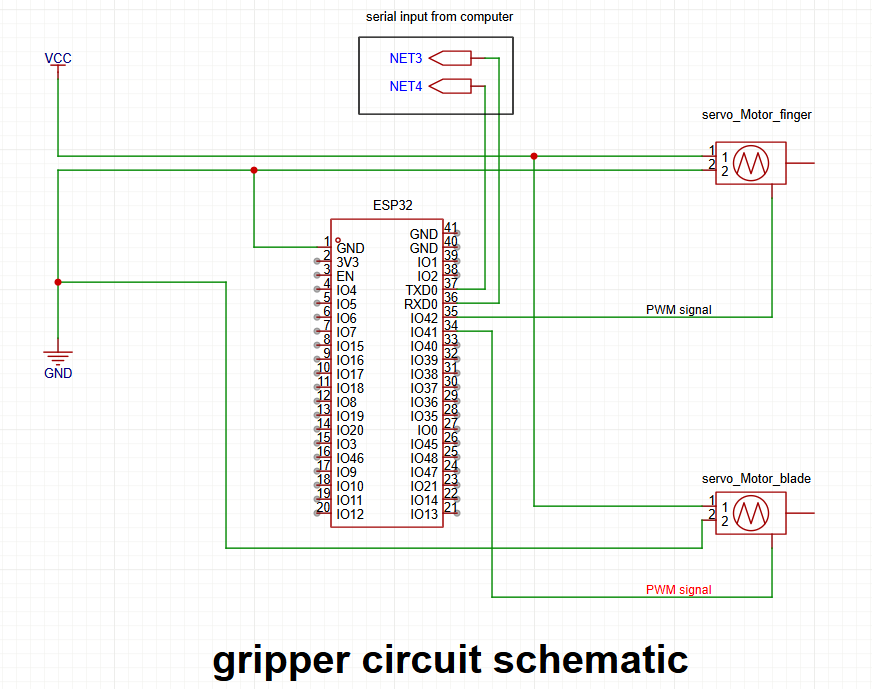
\includegraphics[width=0.9\textwidth]{gripperschamatics.png}
    \caption{Electrical schematic of the gripper controller based on ESP32.}
    \label{fig:gripper_schematic}
    \end{figure}

Figure~\ref{fig:gripper_schematic} presents the electrical schematic for the gripper subsystem. The
ESP32 serves as the central controller and receives high-level commands either via a wired serial
link from a host computer or through Bluetooth Serial communication. A real-time operating system
(RTOS) is employed to schedule the two principal tasks—finger actuation and cutting blade
actuation—so that each executes without blocking or degrading the performance of the other.

Pulse–width modulation (PWM) signals are generated directly by the ESP32 to command the servos.
The finger servo (MG992) is driven from pin IO42, while the blade servo is driven from pin IO41.
These assignments allow independent, deterministic control of grasping and cutting actions, with
timing guarantees provided by the RTOS tasks.

The gripper electronics are powered by a regulated 5\,V supply sized to accommodate concurrent
servo transients; the servo ground is tied to the ESP32 logic ground to ensure a common reference
for PWM signalling. Reference firmware and the associated GitHub repository link are provided
in the Appendix for reproducibility and implementation details.




\section{End-effector fabrication and assembly}

This section documents the physical realisation of the gripper and cutter. Printed parts were
fabricated with fine layers for contact surfaces and higher infill for load-bearing features, then
post-processed by drilling/reaming critical holes to final size. The figures below summarise key
subassemblies and the final integration.


\begin{table}[H]
    \centering
    \caption{Bill of materials for the prototype gripper and cutter.}
    \label{tab:gripper_bom}
    \resizebox{\textwidth}{!}{%
    \begin{tabular}{l c l l}
        \hline
        \textbf{Item} & \textbf{Qty.} & \textbf{Specification} & \textbf{Function} \\
        \hline
        ESP32 development board & 1 & Wi‑Fi/Bluetooth MCU & Central controller, PWM generation \\
        Servo motor (MG995) & 2 & Metal gear, high torque & Finger actuation; blade actuation \\
        Cutting blade & 1 & Utility/trapezoidal blade & Stem cutting element \\
        PLA filament & — & 1.75\,mm, standard grade & Structural parts: gripper and housing \\
        TPU filament & — & 1.75\,mm, shore 95A (approx.) & Compliant soft fingertip pads \\
        \hline
    \end{tabular}%
    }
    \end{table}

The ESP32 provides integrated wireless connectivity and sufficient timers for dual PWM outputs,
enabling deterministic control of both servos. MG995 units were selected for their readily available
torque capacity and robustness for prototyping. PLA is used for the primary structure due to its
dimensional stability and ease of printing, while TPU is employed at the fingertip interfaces to
introduce compliance that distributes contact pressure and mitigates damage to the asparagus spear.
The replaceable utility blade affords a sharp, low-mass cutting edge suitable for repeatable stems
severing during trials.



\begin{figure}[H]
    \centering
    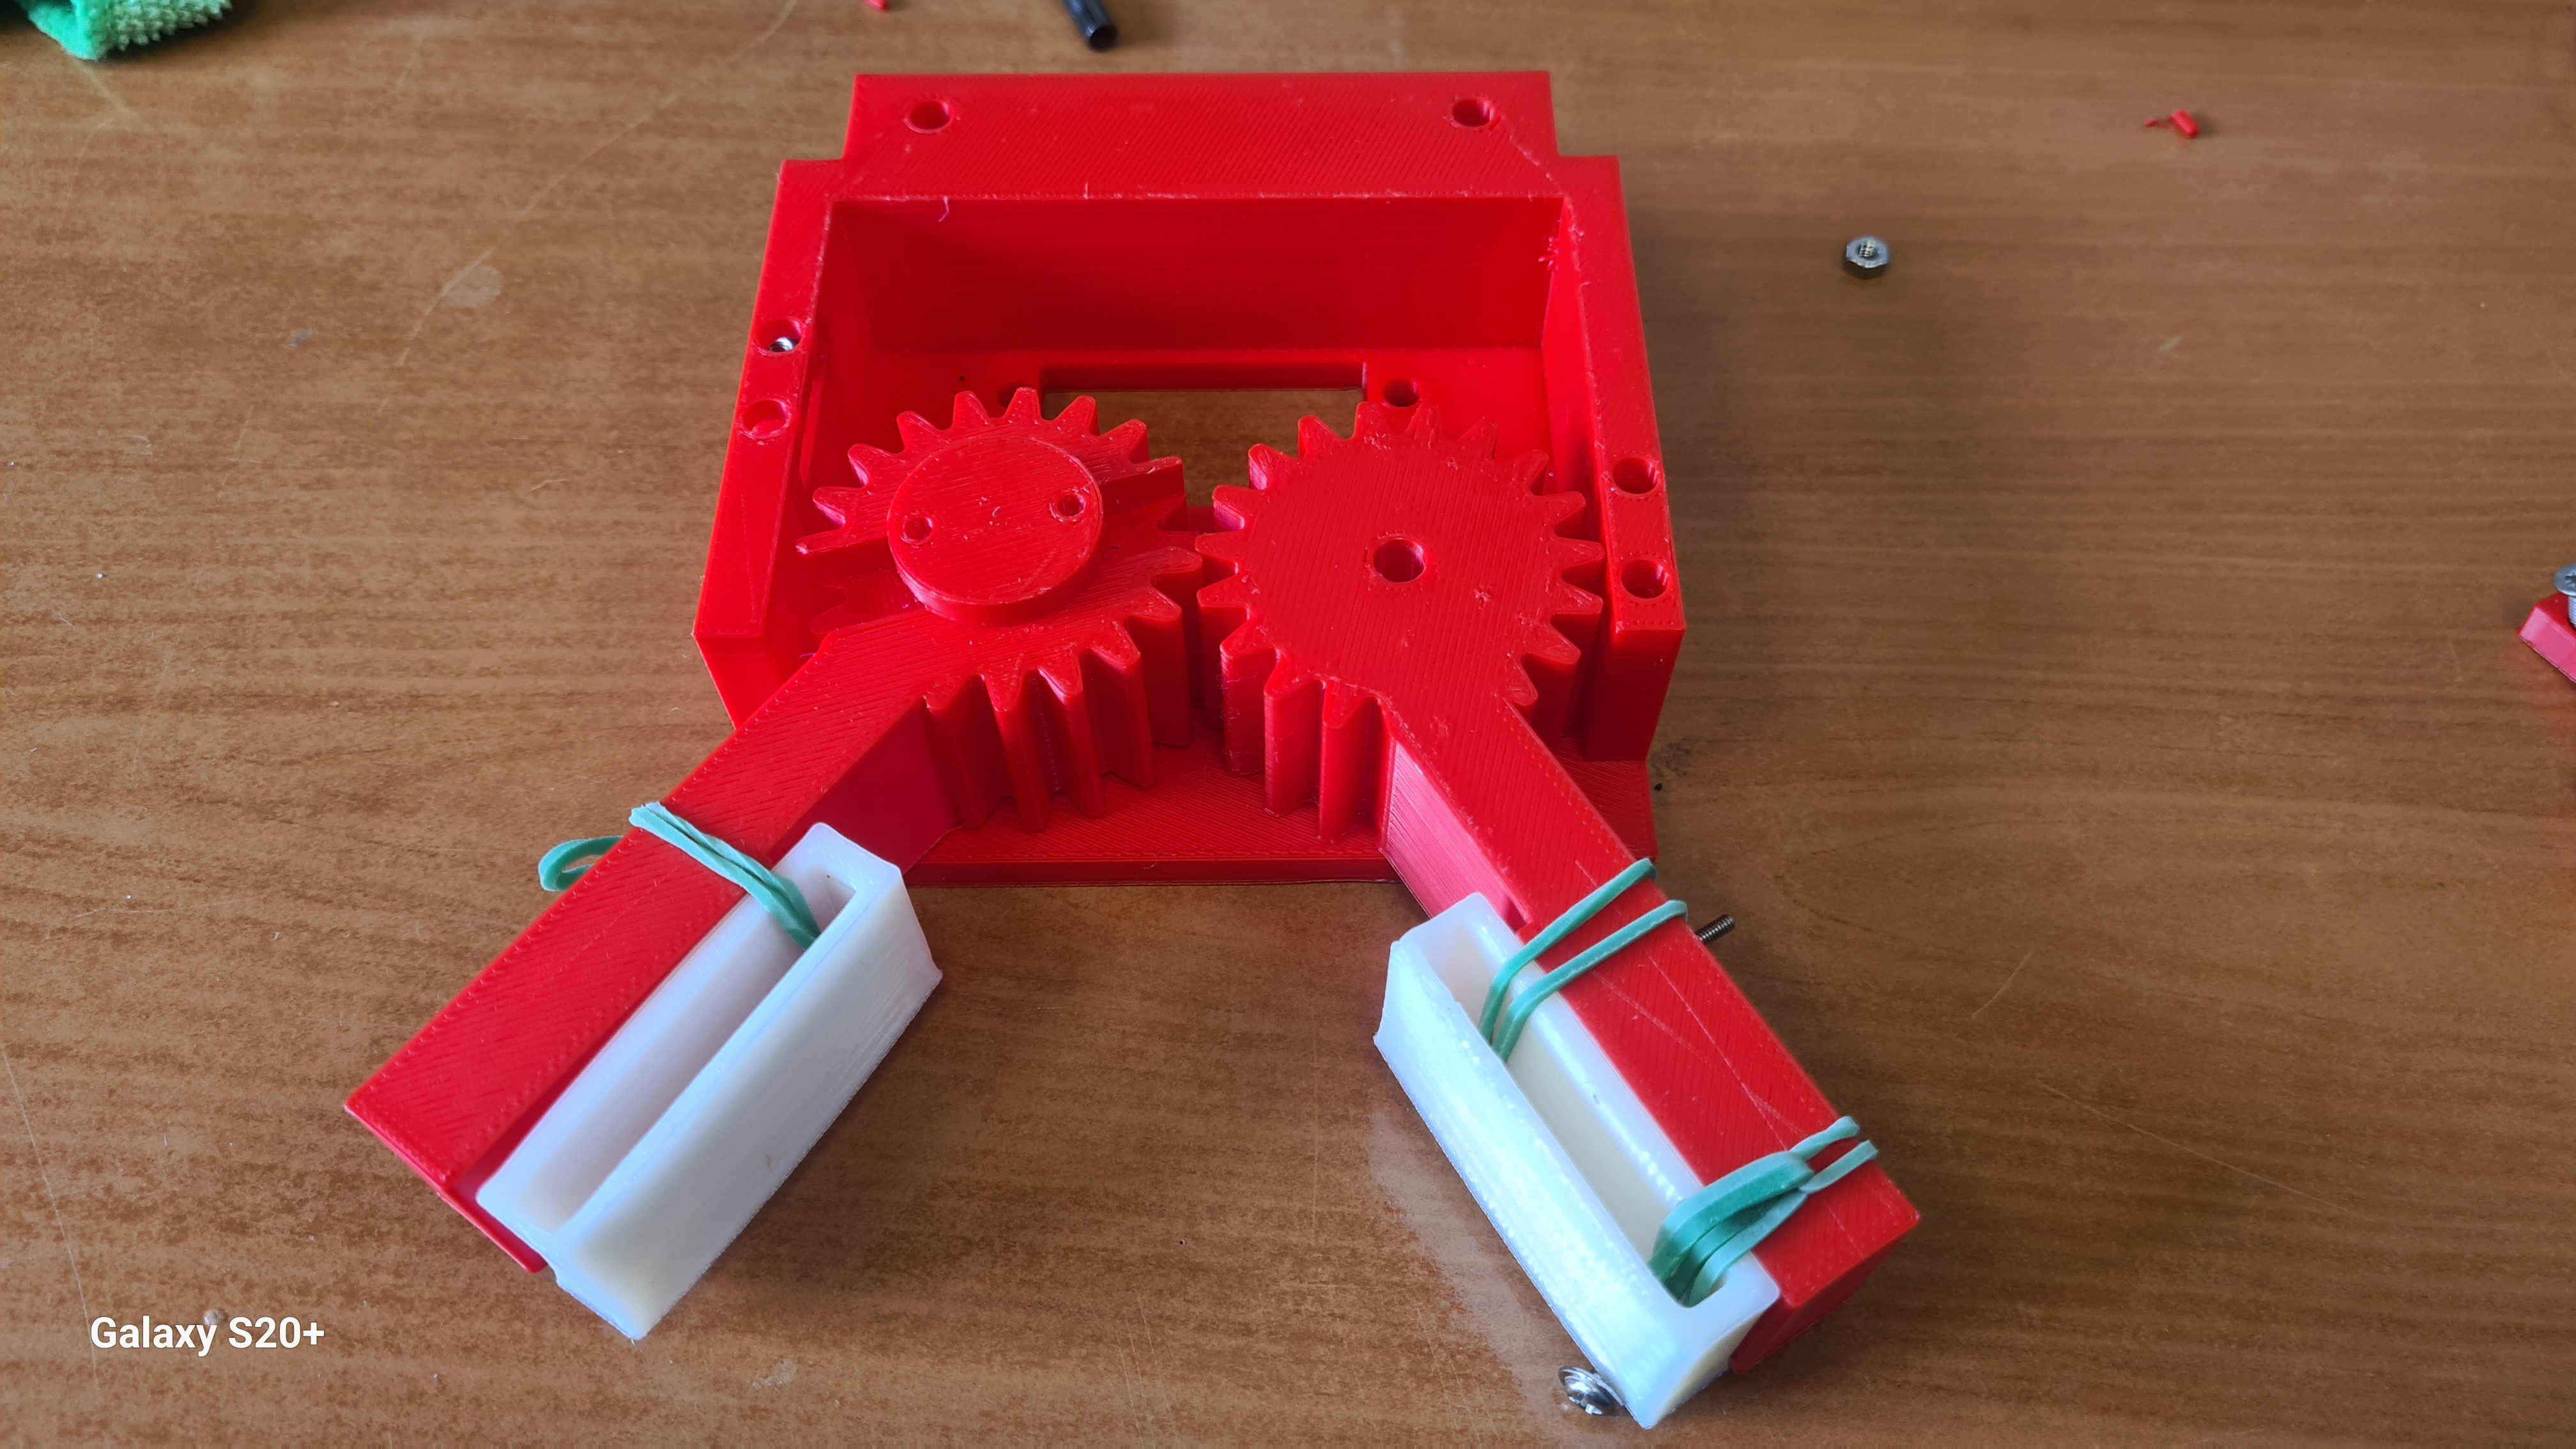
\includegraphics[width=0.9\textwidth]{fingerGear.jpg}
    \caption{Finger actuation gears illustrating the symmetric closing mechanism.}
    \label{fig:finger_gears}
    \end{figure}
    
    Figure~\ref{fig:finger_gears} depicts the printed spur-gear pair used to kinematically
    synchronise the two fingers. The arrangement enforces equal and opposite angular motion,
    yielding symmetric closing and reliable centring of the spear prior to cutting. Gear modules
    and tooth counts were selected to balance compact packaging with adequate torque capacity;
    backlash was minimised through post-processing of bores and the use of press-fit pins with
    lubrication applied after assembly. This configuration reduces differential slip at the contacts
    and improves repeatability of the grasping pose across cycles.
    

\begin{figure}[H]
\centering
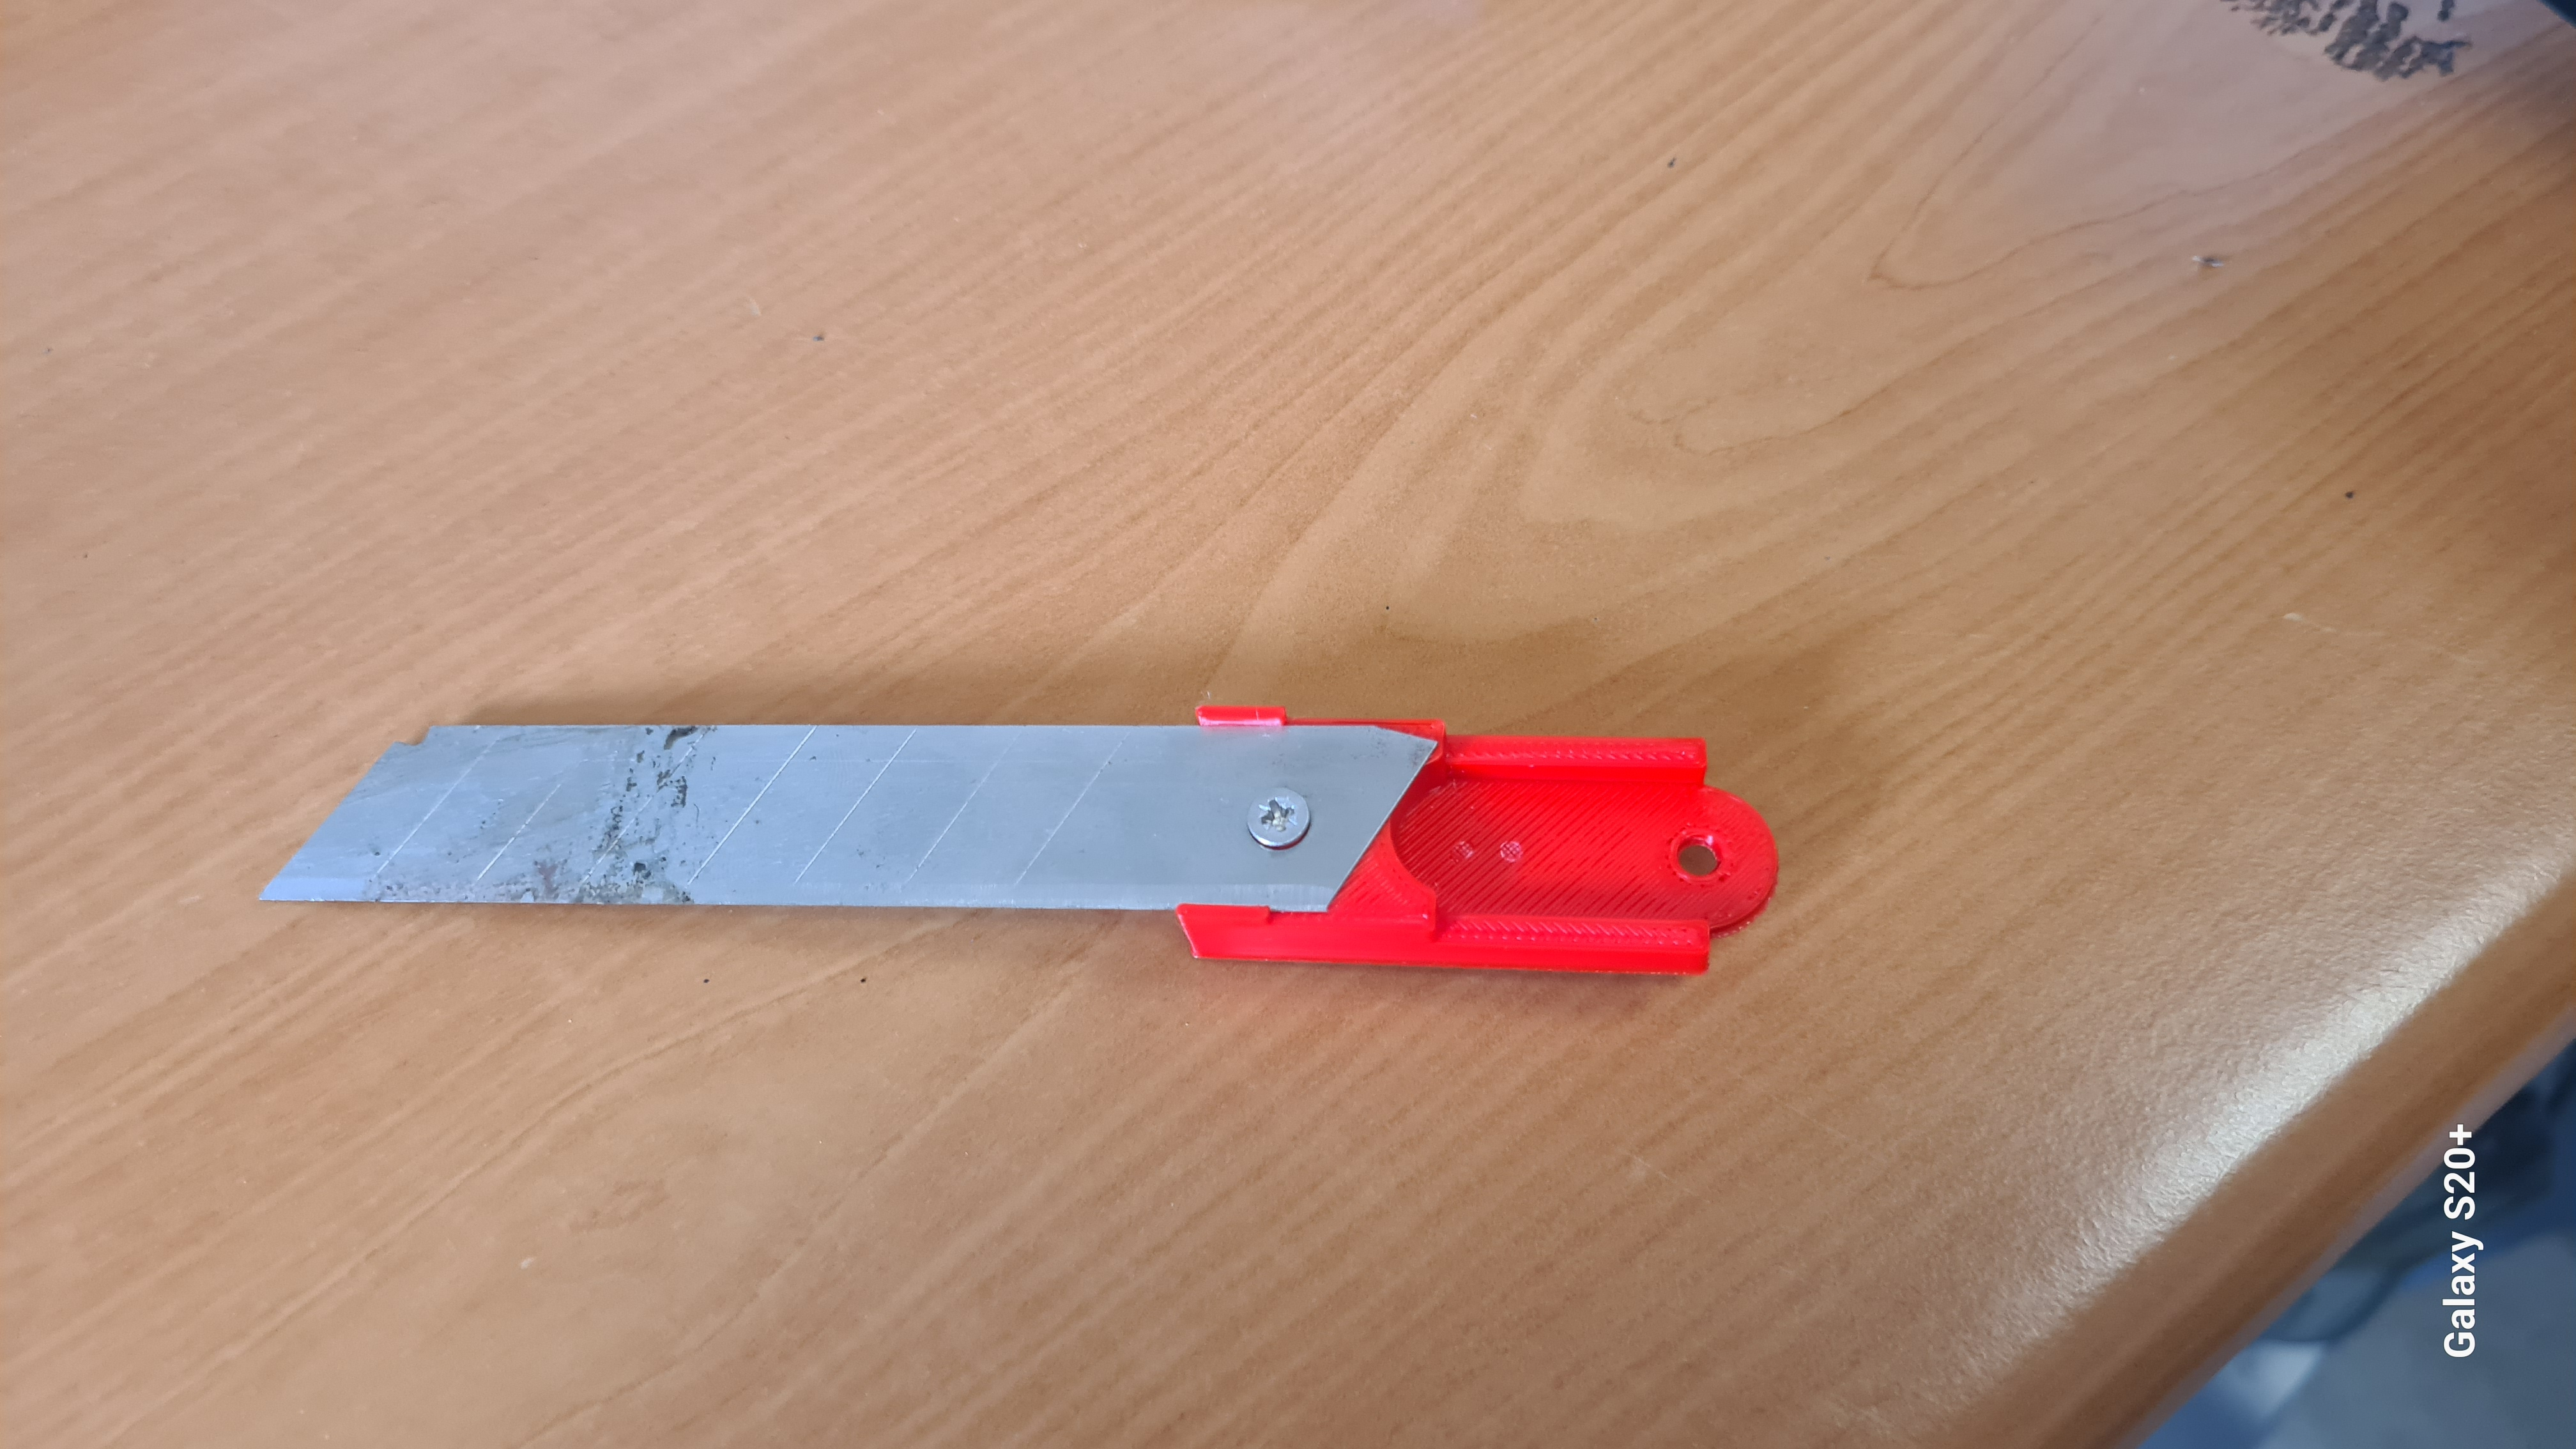
\includegraphics[width=0.75\textwidth]{Blade.jpg}
\caption{Blade prototype for asparagus stem cutting.}
\label{fig:blade}
\end{figure}

Figure~\ref{fig:blade} shows the replaceable utility blade secured within a low-mass carrier used
for early trials. A standard trapezoidal blade was selected for availability, edge sharpness, and
cost. The carrier constrains the blade in-plane while allowing straightforward replacement,
facilitating iterative testing of attack angle and exposure. Preliminary trials focused on edge
durability, required stroke force, and the effect of blade orientation on cut quality.

\begin{figure}[H]
\centering
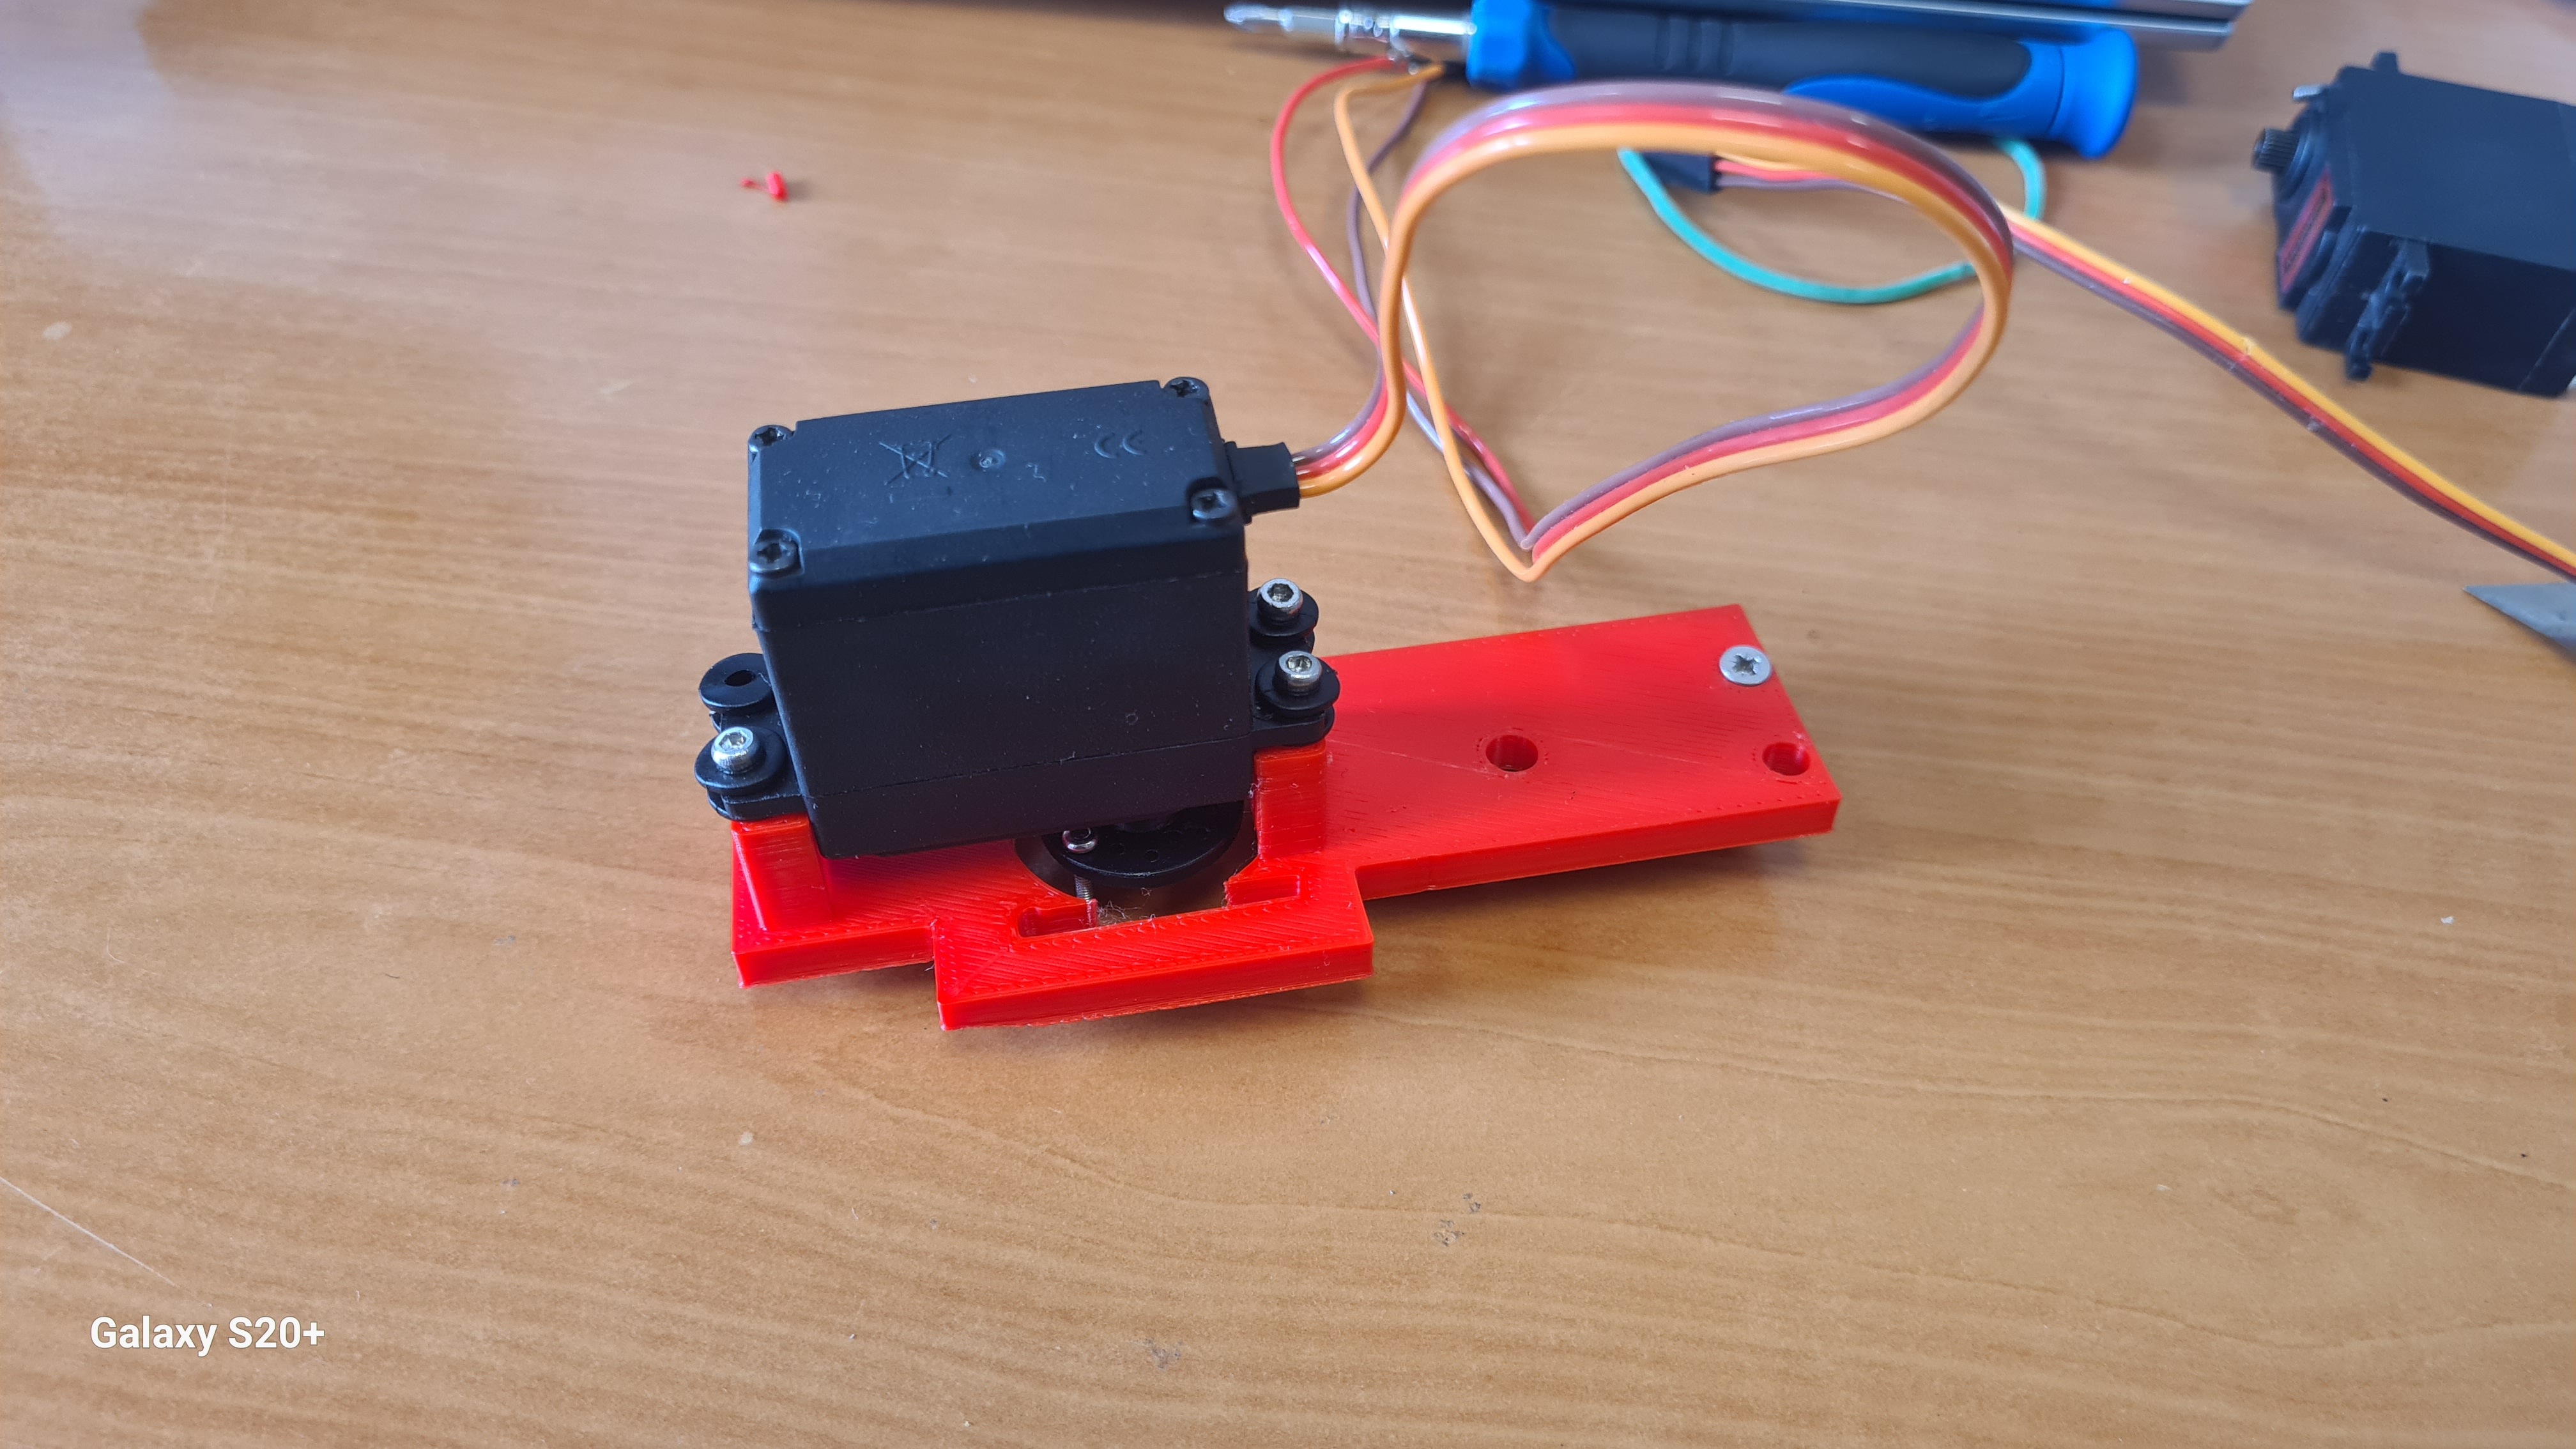
\includegraphics[width=0.85\textwidth]{bladeDriverandMount.jpg}
\caption{Blade driver and mounting arrangement with servo actuation.}
\label{fig:blade_driver_mount}
\end{figure}

Figure~\ref{fig:blade_driver_mount} illustrates the servo-driven blade mount. The blade carrier is
coupled to a high-torque servo through a rigid hub and supported by bushings to constrain
out-of-plane motion. The mount geometry establishes a repeatable attack angle relative to the
stem and limits lateral compliance that could degrade cut quality. Cable routing and fastener
access were considered to enable maintenance and rapid blade exchange during field operation.

\begin{figure}[H]
\centering
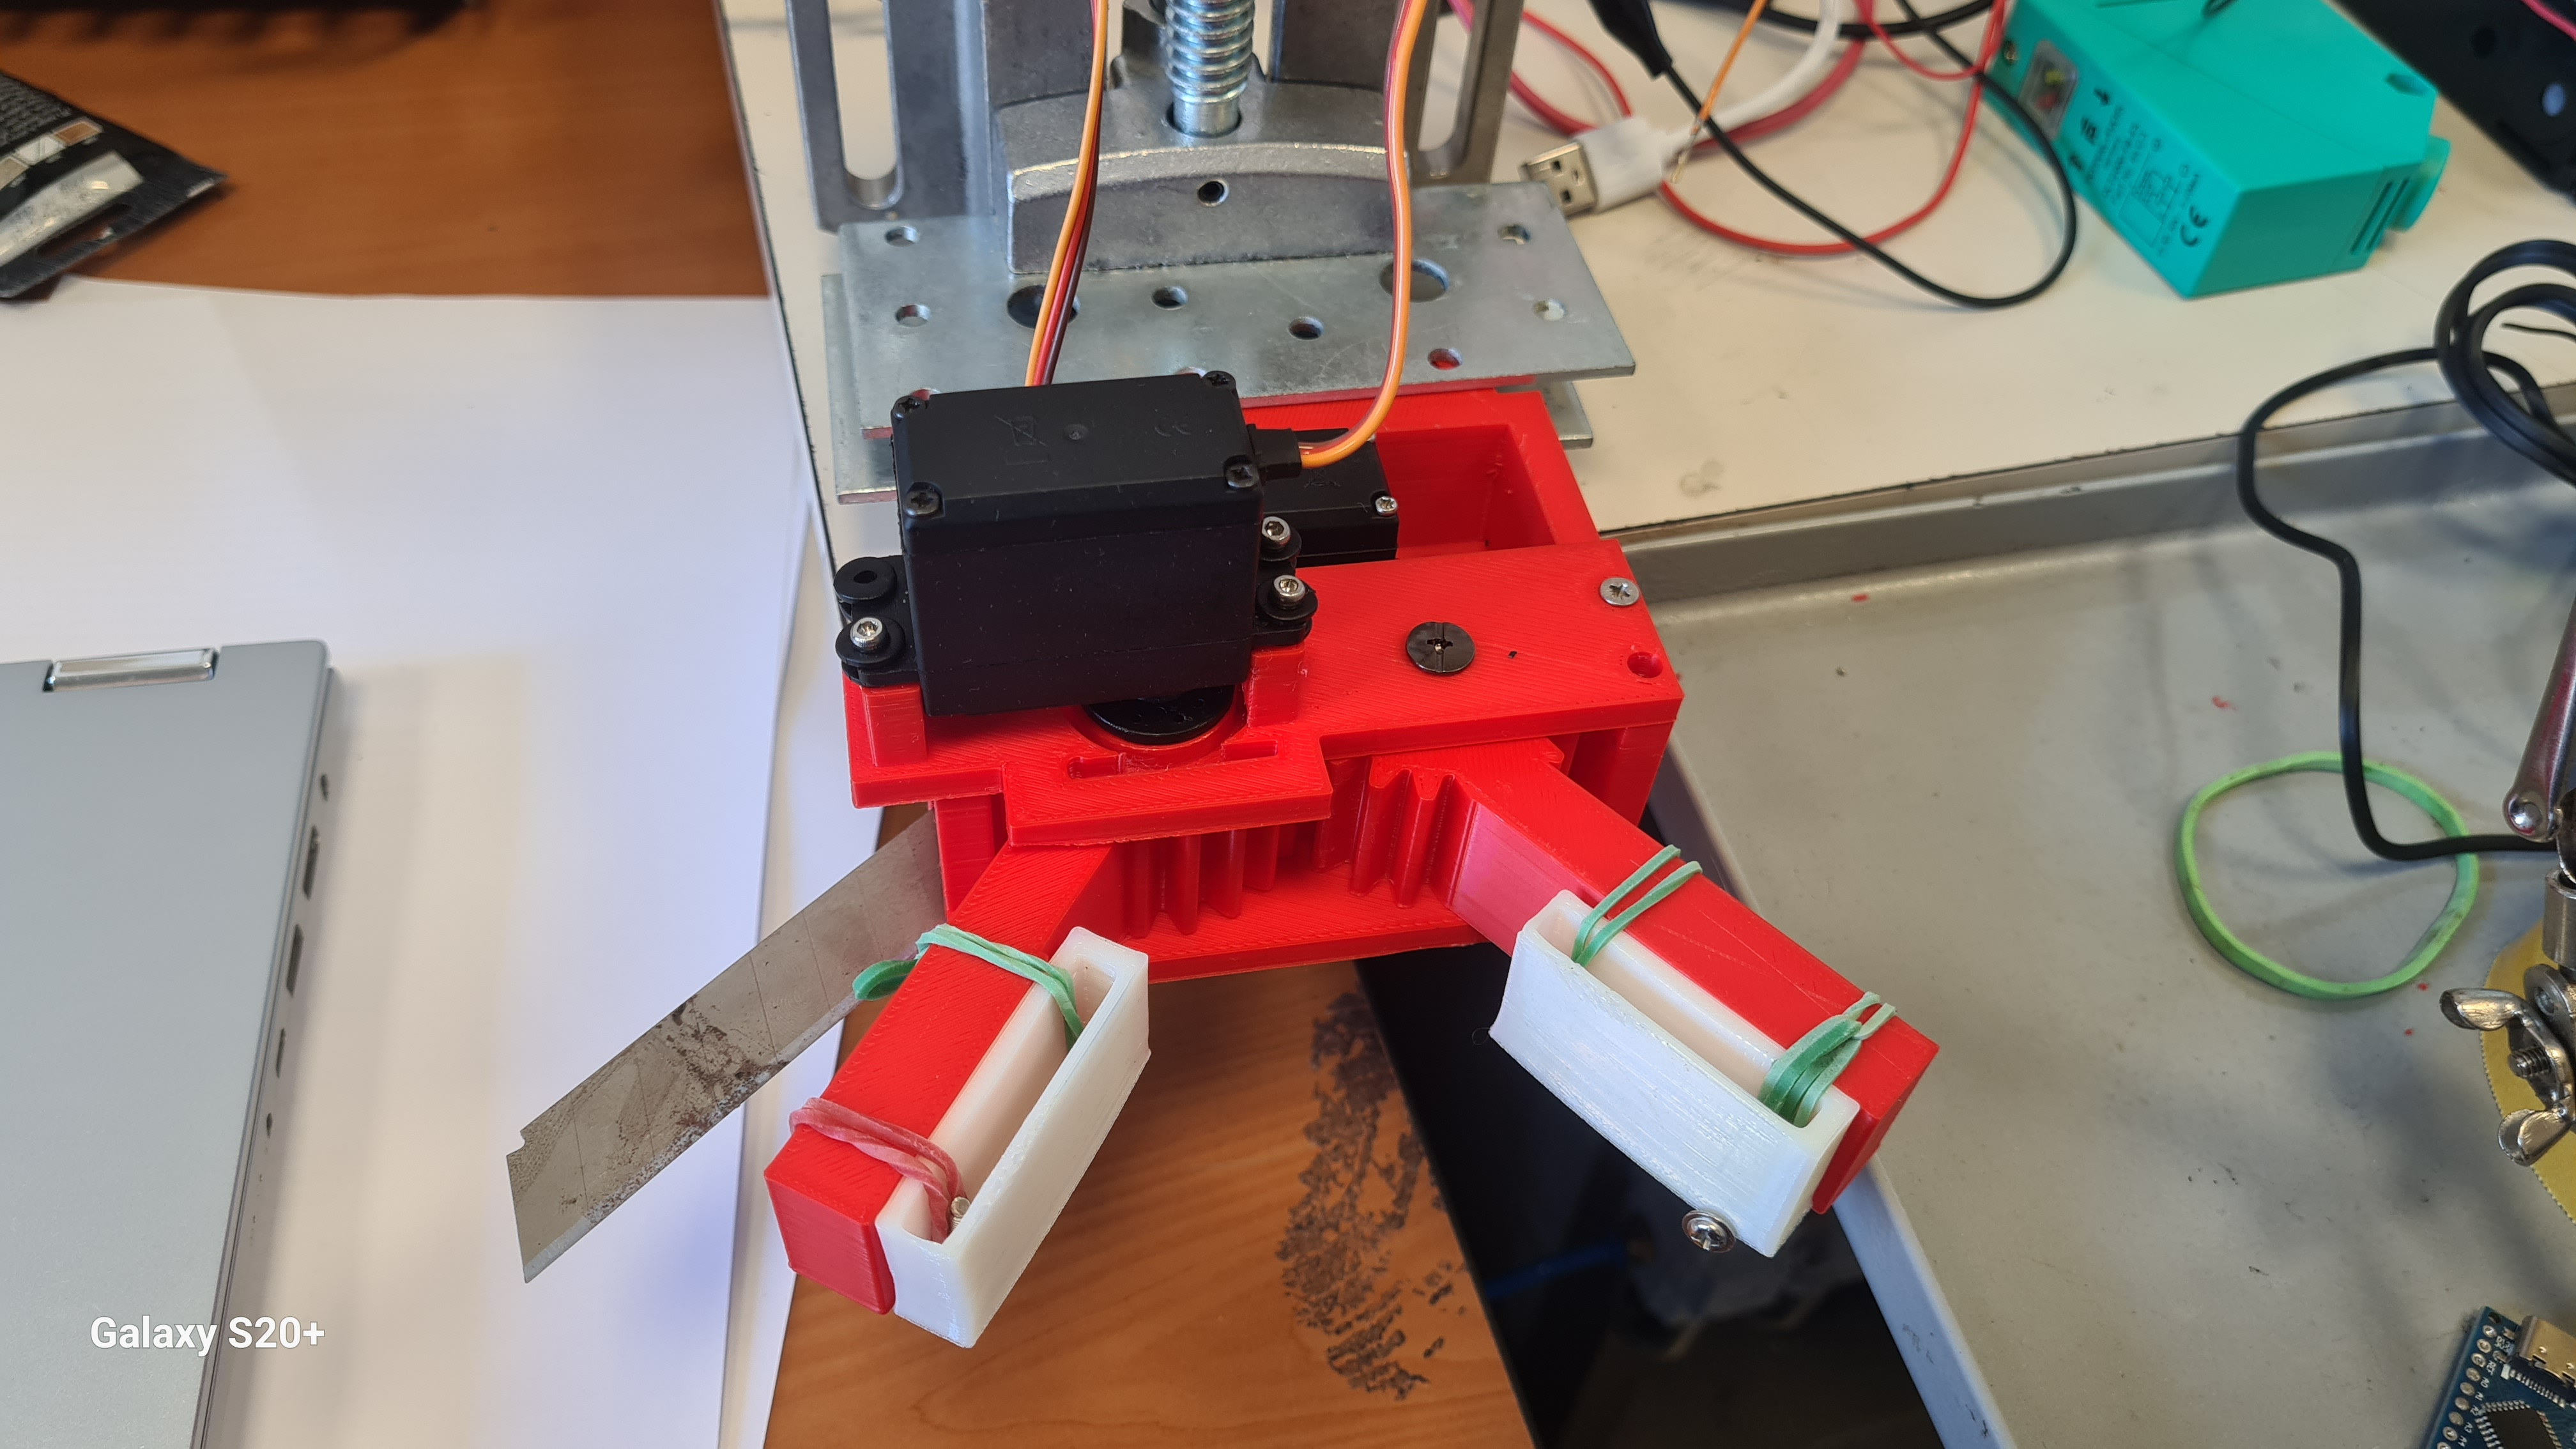
\includegraphics[width=0.85\textwidth]{Fingerfinal_design.jpg}
\caption{Assembled finger and blade module prototype.}
\label{fig:finger_final}
\end{figure}

Figure~\ref{fig:finger_final} shows the final assembly of the finger and blade module. The finger
pair is synchronised via the internal gear train and fitted with compliant pads to distribute
contact pressure, while the blade subassembly is mounted on a rigid bracket driven by a
high-torque servo.The material used for the pad is flexible filament which bends inwards under the pressure and thus does not damage the asparagus stem.The mechanical packaging preserves a compact envelope around the tool
centre point, ensuring that the cutting stroke clears the finger workspace and that cable
routing remains unobstructed. Assembly choices emphasised maintainability: the blade is
readily replaceable, servos are accessible for calibration, and all critical joints are supported by
bushings or bearings to limit wear. The design provides smooth, symmetric closing,
repeatable centring of the spear, and consistent cut quality across repeated cycles, indicating
that the prototype satisfies the principal design objectives for gentle, reliable harvesting.





\chapter{Computer vision}
\section{Requirements of objective}
Automated asparagus harvesting necessitates reliable perception to locate, assess, and safely manipulate spears within complex field conditions. Computer vision provides the sensing and interpretation capabilities required to: (i) detect spears amidst cluttered foliage and soil background; (ii) estimate ripeness or cut-readiness based on geometric and visual cues; (iii) localize targets in three dimensions for tool approach and cutting; and (iv) operate robustly under variability in illumination, occlusions, plant morphology, and weather. In this context, perception performance directly constrains the achievable throughput, product quality, and operational safety of the harvesting system.

The primary requirements are summarized as follows:
\begin{itemize}
  \item \textbf{Detection accuracy}: High precision and recall to minimize missed harvestable spears and false positives that could cause damage.
  \item \textbf{Spatial localization}: Centimeter-level 3D pose (position and, where relevant, orientation) sufficient for motion planning of the end effector.
  \item \textbf{Readiness assessment}: Discrimination between harvestable and non-harvestable spears using measurable features (e.g., height above soil, thickness, tip morphology).
  \item \textbf{Environmental robustness}: Tolerance to shadows, direct sunlight, moisture, dust, and partial occlusions from leaves or neighboring spears.
  \item \textbf{Computational efficiency}: Near real-time inference compatible with the platform's compute and energy budgets.
  \item \textbf{Scalability and maintainability}: Methods that generalize across cultivars, growth stages, and fields with limited re-calibration.
  \item \textbf{Safety and compliance}: Conservative behavior near humans and plants; perception outputs support fail-safe planning and execution.
\end{itemize}

To meet these requirements, this work uses camera-based sensing for both 2D appearance cues and 3D geometric reasoning. The approach integrates image acquisition, camera calibration, point-cloud generation, and segmentation to produce actionable targets for manipulation.

\section{Dataset collection and  model training}
A web-sourced image corpus of 200 asparagus scenes was curated and annotated using the COCO methodology to enable instance-level learning. 
Images were intentionally selected to span challenging, field-relevant variability, including cluttered arrangements and occlusions among 
spears, out-of-focus and mild motion-blur cases, diverse viewpoints and backgrounds, and a broad range of illumination conditions (e.g., 
backlighting, hard shadows, and mixed artificial/ambient lighting). The dataset was partitioned at the image level into non-overlapping 
training (80\%) and test (20\%) splits while preserving the distribution of scene characteristics across splits to reduce evaluation bias.
This diversity is intended to promote robustness and generalization of the Detectron2 models trained in subsequent experiments (see Figure~\ref{fig:dataset_samples}).

Training uses Detectron2's Mask R-CNN with a ResNet-50 backbone and Feature Pyramid Network ,
initialized from COCO-pretrained weights. No validation dataset is attached to the training loop. The model is optimized on CPU with two
 data-loading workers, a base learning rate of \(2.5\times10^{-4}\), and a fixed schedule without decay for a total of 300 iterations. The ROI heads
 are configured for a single foreground category (asparagus spear), with batch size of 128 to balance computation and convergence
 stability for this dataset size. The total training time on Google Colab was approximately 5.3 hours.

\begin{figure}[H]
\centering
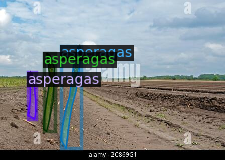
\includegraphics[width=0.48\linewidth]{asp_sample_1.png}\hfill
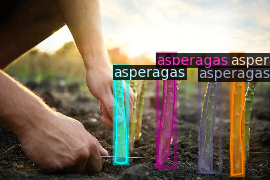
\includegraphics[width=0.48\linewidth]{asp_sample_2.png}\\[0.5em]
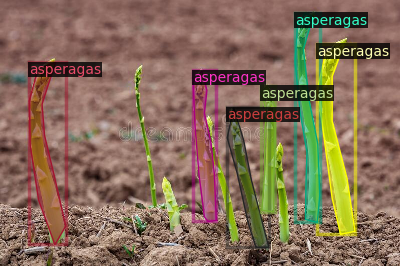
\includegraphics[width=0.48\linewidth]{asp_sample_3.png}\hfill
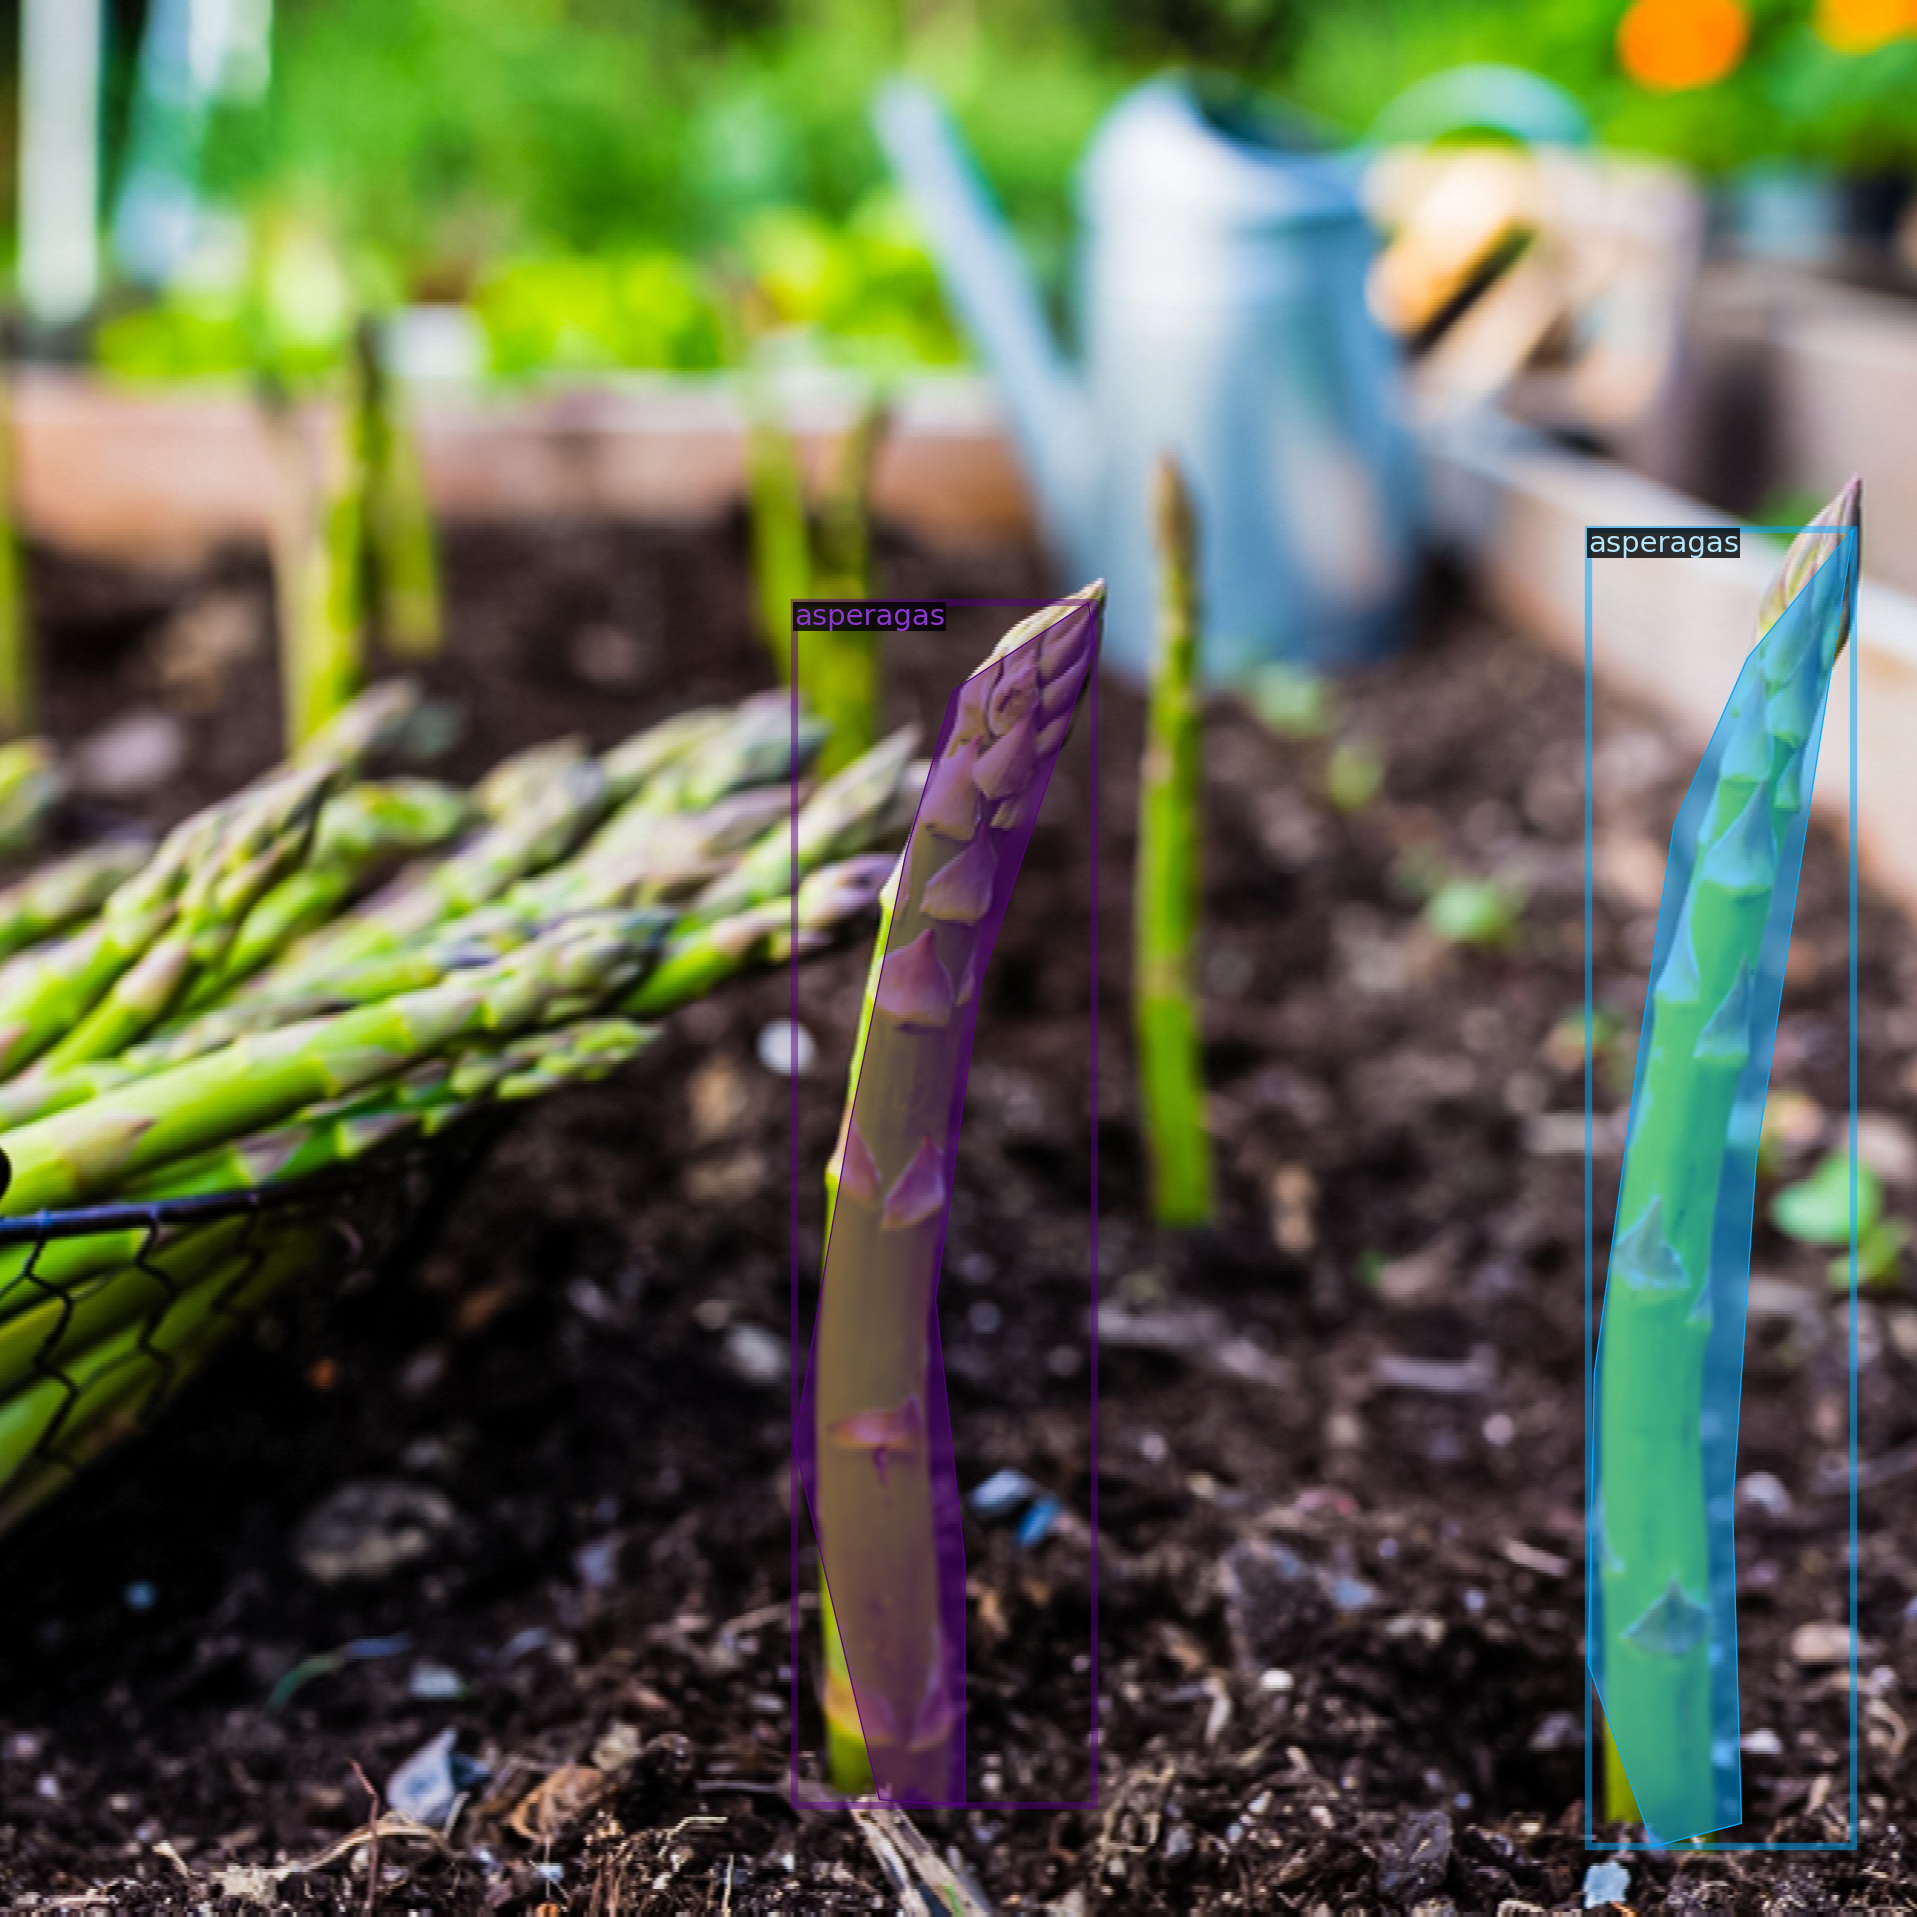
\includegraphics[width=0.48\linewidth]{asp_sample_4.png}
\caption{Representative training samples illustrating variability in clutter, focus, viewpoint, background, and illumination within the dataset described above.}
\label{fig:dataset_samples}
\end{figure}


After training, the model is exported as a TorchScript artifact for deployment and used for inference on the held-out test split. A confidence
threshold of 0.85 is applied for instance selection. On the test dataset, the model achieves an overall detection accuracy above 98.4\%.
Representative qualitative results are shown in Figure~\ref{fig:inference_results}.

\begin{figure}[H]
\centering
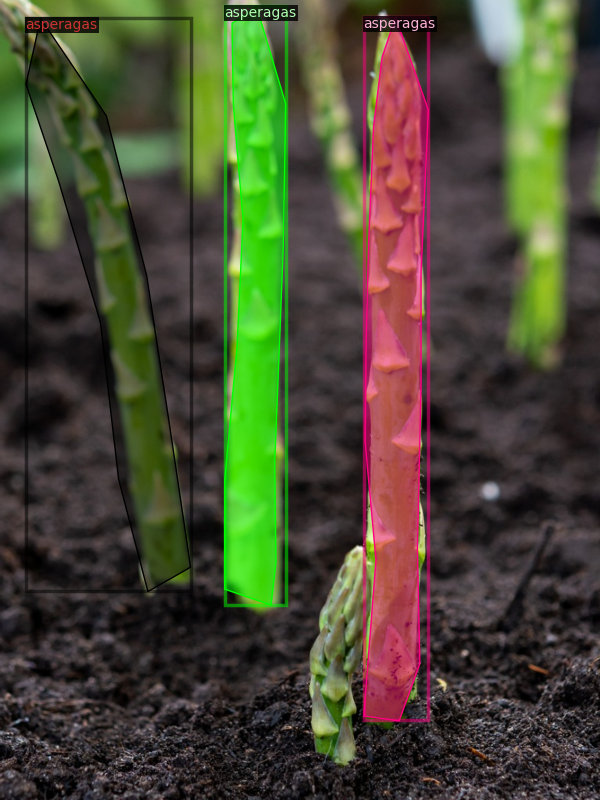
\includegraphics[width=0.48\linewidth]{test_image.png}\hfill
\includegraphics[width=0.48\linewidth]{\detokenize{test_image (2).png}}
\caption{Qualitative inference results on held-out test images. Detected asparagus spears are shown with instance masks and bounding boxes, illustrating robust performance under varied backgrounds and illumination.}
\label{fig:inference_results}
\end{figure}



\section{camera setup in lab environment}
 The laboratory configuration replicates typical field viewing geometry while providing controlled and repeatable imaging conditions. The camera is 
 rigidly mounted on an aluminum extrusion frame using a vibration-damped bracket, with the optical axis oriented obliquely toward the 
 crop bed at an incidence angle of approximately 25--35 degrees. The working distance is set such that a single frame covers the full 
 spear length from soil interface to tip with a 10--20\% margin, ensuring both context and sufficient pixel density for fine structures.

 Intrinsic calibration (focal length, principal point, and lens distortion) is performed following a standard  procedure advised by 
 the manufacturer of the camera; extrinsic calibration to the robot base is obtained via hand--eye calibration with a fixed calibration
  artifact placed at known locations within the workspace.  All transforms are stored and validated at the beginning of each session.

 Illumination is standardized using diffuse LED panels positioned to minimize specular highlights and cast shadows.

 Image acquisition is configured at a constant resolution and frame rate suitable for downstream processing latency. A measurment tape is
 used  in the field of view for periodic verification of metric accuracy. All data are logged with session metadata (calibration parameters, lighting
 settings, and environmental notes) to enable reproducibility. A figure illustrating the physical arrangement of the camera, lighting,
 and sample placement will be provided in this section.

\section{cloud point generation and processing}
Depth information is converted into a 3D point cloud through back-projection using the calibrated intrinsics. Each pixel with valid depth \(d\) at image coordinates \((u, v)\) is mapped to a camera-frame point \(\mathbf{p}_c = d\,K^{-1}[u\ v\ 1]^\top\), where \(K\) is the intrinsic matrix. Points are then transformed into the robot frame via the known extrinsics. Color values are optionally associated to each 3D point for appearance--geometry fusion.

To enhance downstream segmentation and localization, the raw cloud undergoes a processing pipeline:
\begin{itemize}
  \item \textbf{Region-of-interest filtering}: Crop to the expected bed and height range to reduce irrelevant background.
  \item \textbf{Downsampling}: Apply voxel-grid filtering to obtain approximately uniform density and lower computation.
  \item \textbf{Ground removal}: Fit and subtract the soil plane using robust estimators (e.g., RANSAC) to isolate above-ground structures.
  \item \textbf{Outlier suppression}: Remove statistical outliers based on neighborhood distances to improve surface smoothness.
  \item \textbf{Normal estimation}: Compute local surface normals for geometric descriptors and later shape reasoning.
\end{itemize}
The resulting cloud provides a compact, denoised representation suitable for spear segmentation and 3D pose extraction.

\section{segmentation}
Segmentation partitions the sensed scene into spear and non-spear regions and, when required, separates individual spears (instance-level segmentation). Two complementary strategies are considered depending on sensing modality and compute budget:
\begin{enumerate}
  \item \textbf{Geometry-first 3D segmentation}: Cluster the filtered point cloud using Euclidean or density-based methods, followed by geometric constraints on cluster height, thickness, and verticality to retain spear-like structures. This approach is robust to color variation and leverages ground-removed geometry.
  \item \textbf{Learning-based image segmentation}: Apply a convolutional neural network for semantic or instance segmentation in 2D (e.g., encoder--decoder architectures). The 2D masks are lifted to 3D via the registered depth to obtain per-spear point sets. This approach captures fine visual cues and handles partial occlusions when sufficient training data are available.
\end{enumerate}

Post-processing includes morphological smoothing, non-maximum suppression for overlapping hypotheses, and temporal association across frames when operating in motion. For each segmented spear, a 3D reference point (e.g., base point above soil or a cut point at a specified height) is estimated by fitting a simple parametric model to the cluster and intersecting with the soil plane. The final output is a set of target poses with confidence scores, which the planning module consumes for execution.


\chapter{Experiments}
This chapter details the empirical evaluation of the perception and manipulation pipeline in both benchtop and integrated robot settings. 
Our objectives are to: (i) verify that the trained detector produces reliable, actionable targets; (ii) validate the grasping and 
cutting strategy on representative specimens; and (iii) quantify end-to-end performance under realistic operating conditions.






\section{Experiments with robot arm}
\subsection*{Objective and setup}
Integrated experiments assess end-to-end performance when the perception module, camera, and 2-DOF robot arm operate together. The camera 
is rigidly mounted and calibrated using the intrinsic and hand--eye procedures described earlier. The work surface replicates bed geometry, 
and safety interlocks limit speed and workspace during testing.

\subsection*{Method}
Upon detection, target poses are transformed into the robot base frame. A Cartesian approach is planned that maintains tool alignment 
with the spear centerline and enforces a minimum clearance from neighboring spears. After grasping, the tool lifts to a safe height. 
For cutting trials, a cut point is computed at a fixed height above the soil plane and executed with a guarded motion.

\subsection*{Evaluation}
Each run records detection latency, planning latency, execution time, total cycle time, and task outcome (grasp-only or grasp-and-cut). 
We also log near-miss events (clearance violations prevented by the controller) and any operator interventions.

\subsection*{Results overview}
The integrated system demonstrated reliable perception-to-action handoff, with stable cycle times and accurate tool placement under the 
tested conditions. The perception module maintained high detection quality (see Computer Vision chapter) and provided targets that resulted 
in smooth approach trajectories. Typical bottlenecks were motion planning under tight clearances and occasional re-plans due to dynamic 
shadows or reflections. Qualitative examples of successful runs are included in the accompanying figures.









\section{Grasping experiments}
\subsection*{Objective and setup}
Grasping trials evaluate the ability of the end-effector to securely grasp and stabilize individual asparagus spears without
damage. Experiments were conducted on a lab bench with fresh spears placed in soil trays to approximate field support conditions.
The camera and lighting followed the configuration described in the Computer Vision chapter to ensure consistency between 
perception and manipulation trials.

\subsection*{Method}
For each scene, the detector infers spear instances and corresponding masks. A grasp pose is generated by fitting a centerline to the instance mask and selecting a grasp band at a fixed offset above the soil plane. Candidate poses are filtered by thickness and verticality constraints, and the highest-confidence feasible pose is dispatched to the controller. The gripper closes to a torque-limited setpoint before lifting slightly to test retention.

\subsection*{Protocol}
\begin{enumerate}
  \item Place a single or multiple spears in varied orientations and spacings.
  \item Acquire an image, run inference, and compute grasp pose(s).
  \item Execute the grasp using the preset approach trajectory and grasp force.
  \item Record success/failure, grasp time, and any visible damage.
  \item Repeat over mixtures of scenes to cover occlusions and illumination changes.
\end{enumerate}

\subsection*{Metrics}
We report grasp success rate (percentage of trials in which the spear is secured and maintained for 3 seconds), visible-damage rate, 
mean time-to-grasp (from image capture to stable grasp), and pose-planning success (percentage of scenes where a feasible grasp pose 
is produced).

\subsection*{Findings}
Across the collected trials, the system consistently generated feasible grasp poses and executed stable grasps on most scenes. 
Failure modes primarily involved severe occlusions near the grasp band or excessive surface moisture causing slippage. Representative 
outcomes and grasp overlays are provided in the results figures.


\chapter{Conclusion}

\Blindtext


\chapter*{Appendix A}
\addcontentsline{toc}{chapter}{\protect\numberline{}Appendix A}

\Blindtext
% \chapter*{Appendix B}
\addcontentsline{toc}{chapter}{\protect\numberline{}Appendix B}

\Blindtext


% ----------------------
% ---- BIBLIOGRAPHY ----
% ----------------------

\printbibliography

\addcontentsline{toc}{chapter}{\protect\numberline{}Bibliography}

% ----------------------
% ---- DOCUMENT END ----
% ----------------------
\end{document}
